\title{オンラインショッピングサイト利用者による\\商品に対するレビューの動向調査}
\author{プロジェクトマネジメントコース\\
ソフトウェア開発管理グループ\\
矢吹研究室\\
1242042\\
齋藤勇也}
\date{}
\begin{document}

\definecolor{dkgreen}{rgb}{0,0.6,0}
\definecolor{gray}{rgb}{0.5,0.5,0.5}
\definecolor{mauve}{rgb}{0.58,0,0.82}

\lstset{
language={Ruby},
basicstyle={\small},
identifierstyle={\small},
commentstyle={\small\itshape\color{dkgreen}},
keywordstyle={\small\bfseries\color{blue}},
ndkeywordstyle={\small},
stringstyle={\small\ttfamily\color{mauve}},
frame={tb},
breaklines=true,
columns=[l]{fullflexible},
numbers=left,
xrightmargin=0zw,
xleftmargin=3zw,
numberstyle={\scriptsize},
stepnumber=1,
numbersep=1zw,
lineskip=-0.5ex
}

\maketitle
%本テンプレートの余白は,卒論マニュアルで指示されたものとは違っているが,1ページあたりの文字数は40文字x40行と,卒論マニュアル通りになっている。文字間隔や行間隔を調整して,余白をマニュアル通りにすることもできるが,それでは文章が読みにくくなるため,このような対応をしている。

%\noindent
□□□□□□□□□■□□□□□□□□□■□□□□□□□□□■□□□□□□□□□■
□□□□□□□□□■□□□□□□□□□■□□□□□□□□□■□□□□□□□□□■
□□□□□□□□□■□□□□□□□□□■□□□□□□□□□■□□□□□□□□□■
□□□□□□□□□■□□□□□□□□□■□□□□□□□□□■□□□□□□□□□■
□□□□□□□□□■□□□□□□□□□■□□□□□□□□□■□□□□□□□□□■
□□□□□□□□□■□□□□□□□□□■□□□□□□□□□■□□□□□□□□□■
□□□□□□□□□■□□□□□□□□□■□□□□□□□□□■□□□□□□□□□■
□□□□□□□□□■□□□□□□□□□■□□□□□□□□□■□□□□□□□□□■
□□□□□□□□□■□□□□□□□□□■□□□□□□□□□■□□□□□□□□□■
□□□□□□□□□■□□□□□□□□□■□□□□□□□□□■□□□□□□□□□■
□□□□□□□□□■□□□□□□□□□■□□□□□□□□□■□□□□□□□□□■
□□□□□□□□□■□□□□□□□□□■□□□□□□□□□■□□□□□□□□□■
□□□□□□□□□■□□□□□□□□□■□□□□□□□□□■□□□□□□□□□■
□□□□□□□□□■□□□□□□□□□■□□□□□□□□□■□□□□□□□□□■
□□□□□□□□□■□□□□□□□□□■□□□□□□□□□■□□□□□□□□□■
□□□□□□□□□■□□□□□□□□□■□□□□□□□□□■□□□□□□□□□■
□□□□□□□□□■□□□□□□□□□■□□□□□□□□□■□□□□□□□□□■
□□□□□□□□□■□□□□□□□□□■□□□□□□□□□■□□□□□□□□□■
□□□□□□□□□■□□□□□□□□□■□□□□□□□□□■□□□□□□□□□■
□□□□□□□□□■□□□□□□□□□■□□□□□□□□□■□□□□□□□□□■
□□□□□□□□□■□□□□□□□□□■□□□□□□□□□■□□□□□□□□□■
□□□□□□□□□■□□□□□□□□□■□□□□□□□□□■□□□□□□□□□■
□□□□□□□□□■□□□□□□□□□■□□□□□□□□□■□□□□□□□□□■
□□□□□□□□□■□□□□□□□□□■□□□□□□□□□■□□□□□□□□□■
□□□□□□□□□■□□□□□□□□□■□□□□□□□□□■□□□□□□□□□■
□□□□□□□□□■□□□□□□□□□■□□□□□□□□□■□□□□□□□□□■
□□□□□□□□□■□□□□□□□□□■□□□□□□□□□■□□□□□□□□□■
□□□□□□□□□■□□□□□□□□□■□□□□□□□□□■□□□□□□□□□■
□□□□□□□□□■□□□□□□□□□■□□□□□□□□□■□□□□□□□□□■
□□□□□□□□□■□□□□□□□□□■□□□□□□□□□■□□□□□□□□□■
□□□□□□□□□■□□□□□□□□□■□□□□□□□□□■□□□□□□□□□■
□□□□□□□□□■□□□□□□□□□■□□□□□□□□□■□□□□□□□□□■
□□□□□□□□□■□□□□□□□□□■□□□□□□□□□■□□□□□□□□□■
□□□□□□□□□■□□□□□□□□□■□□□□□□□□□■□□□□□□□□□■
□□□□□□□□□■□□□□□□□□□■□□□□□□□□□■□□□□□□□□□■
□□□□□□□□□■□□□□□□□□□■□□□□□□□□□■□□□□□□□□□■
□□□□□□□□□■□□□□□□□□□■□□□□□□□□□■□□□□□□□□□■
□□□□□□□□□■□□□□□□□□□■□□□□□□□□□■□□□□□□□□□■
□□□□□□□□□■□□□□□□□□□■□□□□□□□□□■□□□□□□□□□■
■■■■■■■■■■■■■■■■■■■■■■■■■■■■■■■■■■■■■■■■
□□□□□□□□□■□□□□□□□□□■□□□□□□□□□■□□□□□□□□□■%文字数チェック用

%\chapter*{謝辞}
%謝辞のコメント(未記入)



\tableofcontents%目次

%\frontmatter
%\tableofcontents
%\mainmatter


\chapter{序論}

1994年に始まったといわれる\cite{sugasaka2003}オンラインショッピングは,全ての商取引における電子取引の割合が2014年時点で3.7%となり,2008年の1.8%比べ 倍近く上昇し\cite{keizai2014},2014年に至るまでに大きく普及していることから仮想空間でも商品の売買が行いやすい環境であることが分かる.

商品を買うという行動に選択肢が増えたことで,商品に対するレビューの仕方にも変化が加わった.オンラインショッピングでは,購入したサイト上で商品のレビューを行うようになったのだ.
オンライン上で商品を販売するオンラインショッピングサイトではレビューは五段階評価で行い,それらレビューを合計し平均値で表示する.しかし,このレビューは記入が自由に行えるため,商品に対して嘘偽り,無関係のレビューを行えることを意味する.

このような嘘偽り,無関係のレビューが存在し,該当するレビューの五段階評価をその評価の状態で計算するオンラインショッピングサイトのレビューでは信頼性が低い.

そこで当研究では,実際に存在するオンラインショッピングサイトを利用し,判断材料としての指標が少ない平均値を上回る信頼性のある評価値を生み出すことを目的とする.

この平均値を上回る信頼性のある評価値を生み出すことで,オンライン上に存在する商品に対して正しい評価を下すことが可能となり,売買においてより信頼できる取引が行える.



\chapter{背景}

インターネットを利用した電子商取引は1994年に米国のピザハットが行ったのが最初であるといわれている\cite{sugasaka2003}.
1994年以前,商品の購入方法は商品の下に足を運ぶ必要があった.つまり商品を購入した人物は直接顔を合わせた相手にのみにしかレビューを語ることが出来ない状態である.

書籍によると全ての商取引における電子取引の割合が2014年時点で3.7%となり,2008年の1.8%比べ 倍近く上昇し,仮想空間でも商品の売買が行いやすい環境であることが分かる\cite{keizai2014}.
仮想空間での商品の売買が可能となった1994年以降は,電子商取引であるオンラインショッピングのレビューが重要視されている.



\begin{figure}[htbp]

\centering
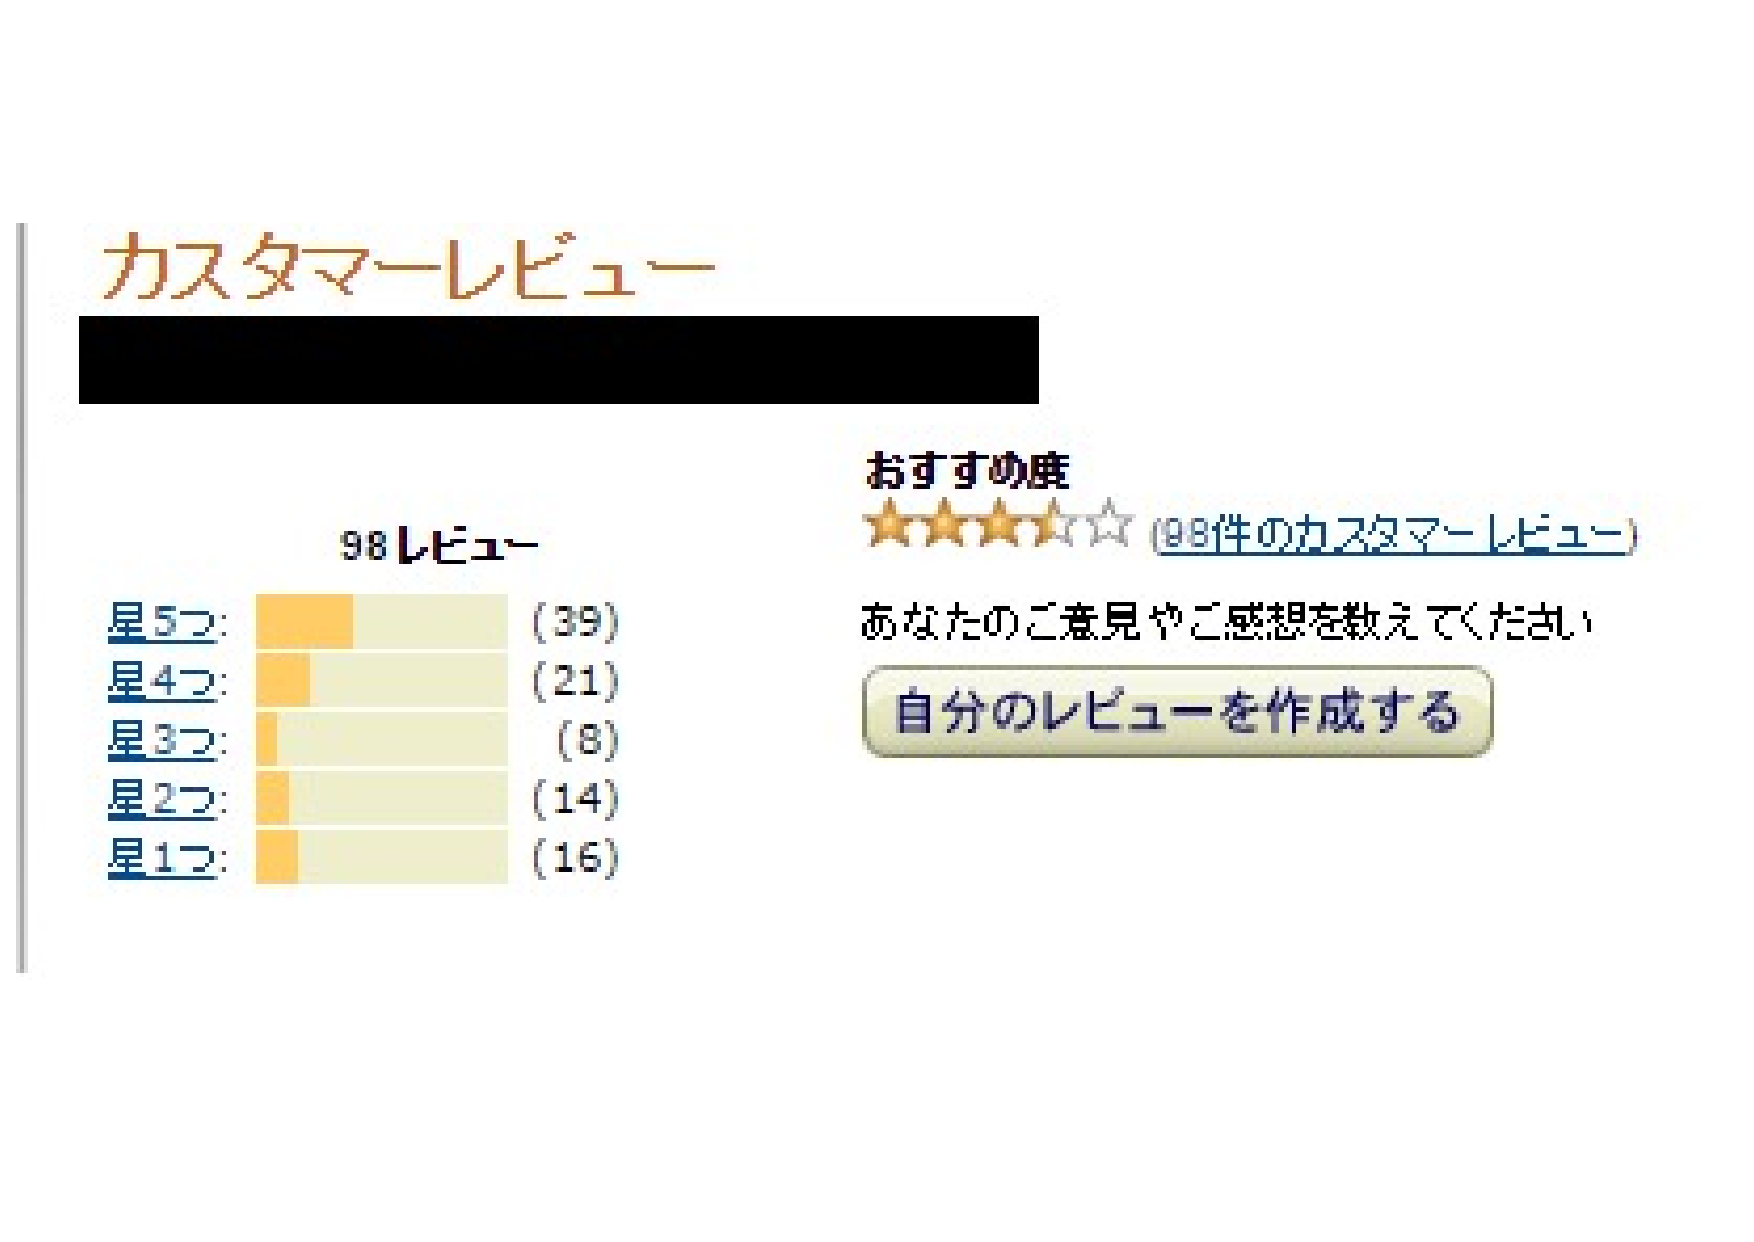
\includegraphics[width=7cm,clip]{customerReview.pdf}
\caption{Amazonでのレビューの一例}
\label{customerReview}

\end{figure}

レビューが実装されている有名なオンラインショッピングサイトでは,利用者は商品についてのレビューを記入することや,商品に得点を付けることが可能である.例えば,Amazonのレビューでは(図\ref{customerReview})おすすめ度と称して平均値しか表示していない.実際に商品とは一切関係のないレビューや明らかに商品に対して理解が足りないレビューがあり,それらのような本来加えるべきでないレビューも多々存在する.

そこで,レビューの表示が平均評価では商品の判断材料としての指標が少ない.そこで平均値のみの表示よりも信頼できる方法を探す \cite{hattori2011} \cite{yamazawa2006}.










\newpage












\chapter{オンラインショッピングサイトについて}

	研究の題名にも記載されているオンラインショッピングサイトにまつわる内容を説明する.


\section{オンラインショッピングサイトとは}

オンラインショップとは、インターネット上で商品を販売するWebサイトのこと.
商品を紹介するWebページを見て購入する商品を選択し,決済方法を指定して住所などの個人情報を送信すると,購入を申し込むことができる.\cite{onlineshop}
決済方法は様々で,代金引換郵便や銀行振込を利用するものから,クレジットカードを利用するもの,あるいは「BitCash」などのいわゆる「電子マネー」システムを利用するものもある.
現状では,大口の決済に適した電子決済手段が確立されておらず、セキュリティ技術も発展途上であることから、電子商店で扱われる商品も数万円以下の比較的安価なものがほとんどである.
扱われる商品の種類は日用品や家電製品などの物品から,保険やサービスまで幅広い.1つのWebサイトにいくつもの電子商店を集めたものを「電子商店街」(オンラインモール)という.


	オンラインショッピングサイトとはインターネット上で商品を販売するWebサイトのことである.
	電子商取引は1994年に米国のピザハットが行ったことを発端に\cite{sugasaka2003},多くのオンラインショッピングサイトが誕生した.
	2015年現在の日本市場は「楽天,Yahoo!,Amazon」などが大手企業として存在している.

\section{オンラインショッピングサイトの起業方法}
現在,オンラインショッピングサイトを作る方法として,11通りある.

そこで個々に1種類ずつ紹介を行うこととする.

\subsection{レンタル・ネットショップ}

レンタル・ネットショップとは,自動車のレンタカーと同く,ネットショップ店舗を借りられるサービスのこと.
申し込めば,陳列棚からレジなど,必要な機能が装備された「空の店舗」が用意され,商品を持ちこめば,その日にでもお店が開店できるサービスだ.

\subsubsection{ネットショップとは}

ネットワークとしての性能が向上し,1家庭あたりのパーソナルコンピュータの所持数の増加が見られる現在では,インターネットを利用した売買がもはや日常的なものとなっている.
その日常化したネットショッピングにも様々な種類が存在する.その様々な種類が存在することを紹介すると同時にネットショッピング特有の運用方法も記載していく.\cite{netshop}

\subsubsection{ネットショッピング開業における手続き,届け出}

\begin{itemize}
 \item	販売不可となる物品の調査

ネットショッピングでは農産物や農家から直送する場合や加工品を仕入れて販売する場合は許可を取る必要はない.
しかし,オーナー自らが加工して販売する場合は,各都道府県の保健所に向けて届出を出す必要がある.

実店舗で運営しているならばすでに保健所の許可を取っている可能性が高いが,自宅で手作りする場合は問題が発生する.
営業するに当たり,自宅以外の台所位阿賀井に専用の厨房施設を設けなければならない,これは届け出を出すことは必須だがそれ以前にスペースと空間をつくりにあたり設備費用がかかるので必ず保健所に相談する必要がある.
またアルコール度数1度以上のお酒を販売する場合には一般逆類小売業の免許とネットで販売するための酒類の通販の免許が必要になる.
中古品を販売する場合には古物商許可証が必要.ペットの場合哺乳類.鳥類,爬虫類を販売する場合には保健所の届け出が必要になる.
ただし,魚類,昆虫類に関しては届け出は不要となる.ペット用の餌を販売する場合も届け出は必要ない.



 \item	免許,許可証が必要になるケースの例
\begin{itemize}
\setlength{\parskip}{3mm}
 \item	手作りのキムチや漬物
 \item	手作り菓子,ケーキ
 \item	手作りジュースやジャム
 \item	魚介類(生・干し物・燻製)
 \item	乳製品(牛乳・チーズ)
 \item	アルコール度数1度以上の酒類すべて
 \item	中身の入ったワインボトルをエッジングなど加工して販売
 \item	みりん
 \item	中古の本やCD,DVD
 \item	中古の家具
 \item	リサイクル衣料品
 \item	アンティーク物の時計,宝石
 \item	チケットや金券
 \item	犬や猫,小鳥などの小動物
 \item	イグアナなどの爬虫類
 \item	花火や爆竹
 \item	ガソリン
 \item	コンタクトレンズなどの医療器具
\end{itemize}



 \item	免許,許可証が不必要なケースの例
\begin{itemize}
\setlength{\parskip}{3mm}
 \item	実家で生産した農産物
 \item	缶詰
 \item	スナック菓子
 \item	お茶やコーヒーなどの飲料
 \item	ブランデーケーキ
 \item	ラムレーズンアイス
 \item	酒饅頭
 \item	ウイスキーボンボン
 \item	奈良漬
 \item	熱帯魚などの魚類
 \item	カブトムシなどの昆虫
 \item	ペットの餌
\end{itemize}
\end{itemize}

\begin{itemize}
 \item	輸入食品による規制事情

商品を輸入して販売する場合にはさらに許認可が必要になる.
食品に関しては国内商品では必要のなかった野菜や果物の農産物から,缶詰,缶ジュースなどの加工済み商品にいたるまで,食品衛生法に基づき届け出が必要となる.
手続きの際には「食品等輸入届出」に必要な書類を付属して厚生労働省検疫所の輸入監視担当に提出して審査,監査を受ける必須である.
口に接触しやすい食器類やベビー用品も同様の手続きが必要となる.この手続きはすべて一人で行うのは難しいため,代行者に依頼することが多い.
植物類の場合哺乳類や鳥類,爬虫類だけでなく国内では認可不要であった昆虫類,魚類にも届出が必要となる.動物の場合は農林水産省の動物検疫所,植物は農林水産省の植物検疫所にて検疫を受ける必要がある.

このほか,輸入品の毛織物,シルクの衣類,ぬいぐるみなどにも注意が必要だ.毛織物は基本的に輸入自由品目だが,ワシントン条約に該当する動物の毛皮を用いたものは,経済産業大臣の輸入承認を得なくてはならない.シルクの布も通常は輸入規制はないが,商品によっては輸入管理体制が実施されている場合もあるので経済産業省の窓口に相談する必要がある.ぬいぐるみも原則自由に輸入できるがワシントン条約に該当する動物の羽毛などを使ったものは輸入できない.また,ミッキーマウスなどの特定のキャラクターは,権利者から税関に対して輸入差し止め申し立てがされており,基本的に輸入できないので注意が必要である.



 \item	免許,許可証が必要になるケースの例
\begin{itemize}
\setlength{\parskip}{3mm}
 \item	農産物
 \item	缶詰などの加工品
 \item	お茶やコーヒーなどの飲料
 \item	お皿や茶碗カップ,グラス
 \item	スプーン,フォーク,ストロー
 \item	種子類
 \item	犬や猫,小鳥などの小動物
 \item	生花
 \item	イグアナなどの昆虫類
 \item	ドライフラワー
 \item	熱帯魚などの魚類
 \item	カブトムシなどの昆虫
 \item	幼児用玩具
 \item	哺乳瓶などの乳児用品
\end{itemize}



 \item	免許,許可証が不必要なケースの例
\begin{itemize}
\setlength{\parskip}{3mm}
 \item	灰皿など

\end{itemize}
\end{itemize}



\subsubsection{ネットショップでの商品の仕入先}

ショップとしての利益を出すにはできるだけ安く仕入れて適正価格で販売するのが基本だ.

\begin{figure}[htbp]

\centering
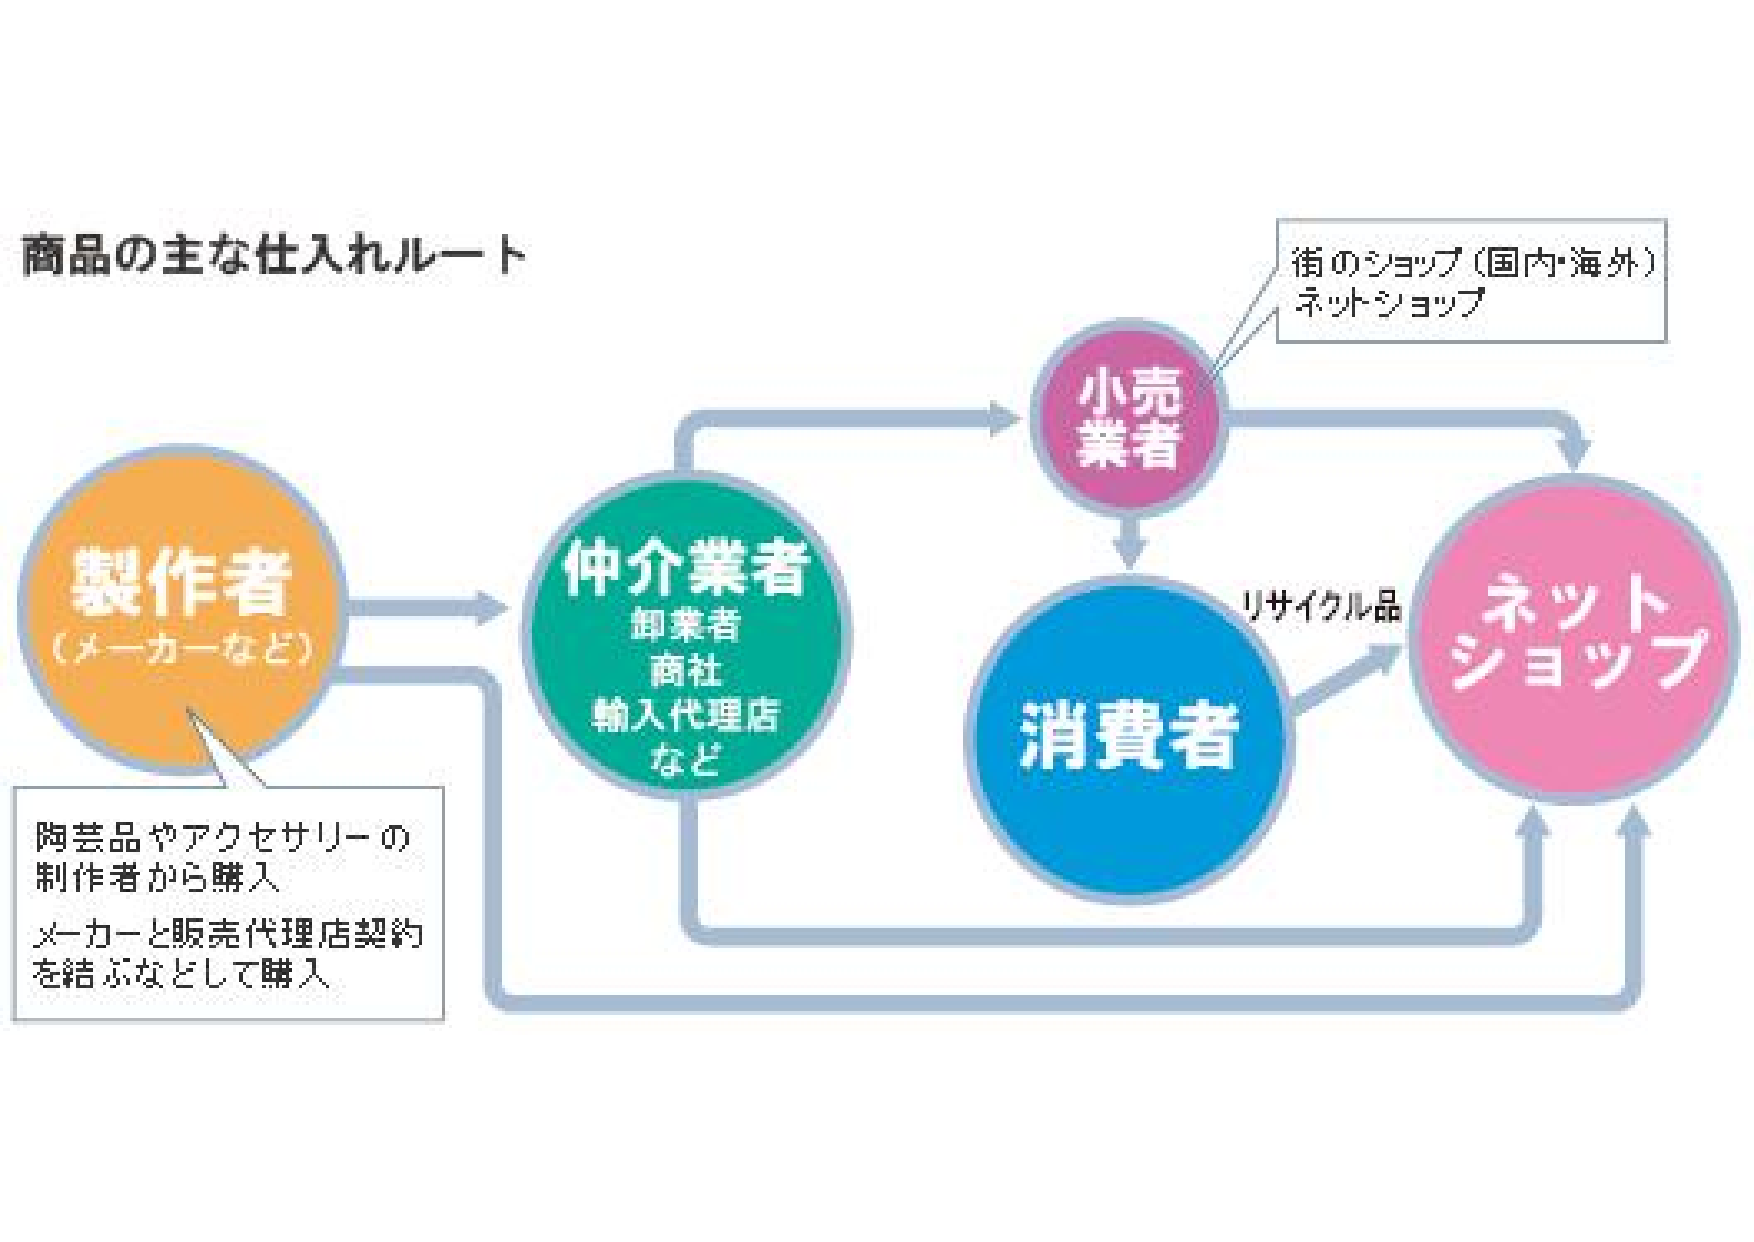
\includegraphics[width=8cm,clip]{netshop.pdf}
\caption{商品の仕入れルート}
\label{netshop}

\end{figure}

製作者は個人の製作だけでなくメーカーも含む.

仲介者を利用する場合法人であれば問題ないが個人事業者のネットショップの場合は取引を行いづらい.ただし,なかには小売りを行う業者もあり,通常の小売店に比べ安い値段で購入できる.数量をまとめて交渉することで,さらに割引価格で仕入れることも可能.

契約に至るまでには次のような段取りが必要になる.(1)面談→(2)契約書類の提出(ネットショップの規模やコンセプト,資金などを記入)→(3)契約内容の確認(初回仕入れは5万円以上.年間30万円の取引など)→(4)契約成立.

最初の3~6カ月はほとんどが「前払い」か「代金引換」となるため,仕入れのための資金は、ある程度確保しておく必要がある.一般的にはこの間の取引で業者からの信頼を得られれば,「月末締めの翌月10日払い」などへと変わる.
小売業者は,卸業者の商品ではバリエーションが少ないという場合に利用するケースもある.その場合卸業者よりも単価が上がるため,利益率が低い.長い目で考えると,小売業者からの仕入れだけでは,ショップ運営は難しい.
リサイクル商品を扱う場合などは、「消費者」から商品を仕入れることもある.この場合,契約を交わすことがないので用意に行えるが,在庫が思うように揃わないというリスクがある.


\begin{itemize}
 \item	商品の仕入先の探し方
\begin{itemize}
\setlength{\parskip}{3mm}
 \item	ネットワーク経由で卸業者を検索する
 \item	メーカとの直接交渉
 \item	実店舗のある卸売業者から直接仕入れる
 \item	展示会に直接足を運ぶ


\end{itemize}
\end{itemize}



\subsubsection{ショップ公開に使用するレンタルサーバー}
ネットショップを開業するには,コンピュータをインターネットに接続し,さらにインターネット上に ネットショップを公開するスペースを確保する必要がある.

インターネットに接続するために必要なのがプロバイダーとの契約であり,ネットショップを公開するのに必要なスペースが専門の事業者と契約して借りるレンタルサーバーである.


\begin{figure}[htbp]

\centering
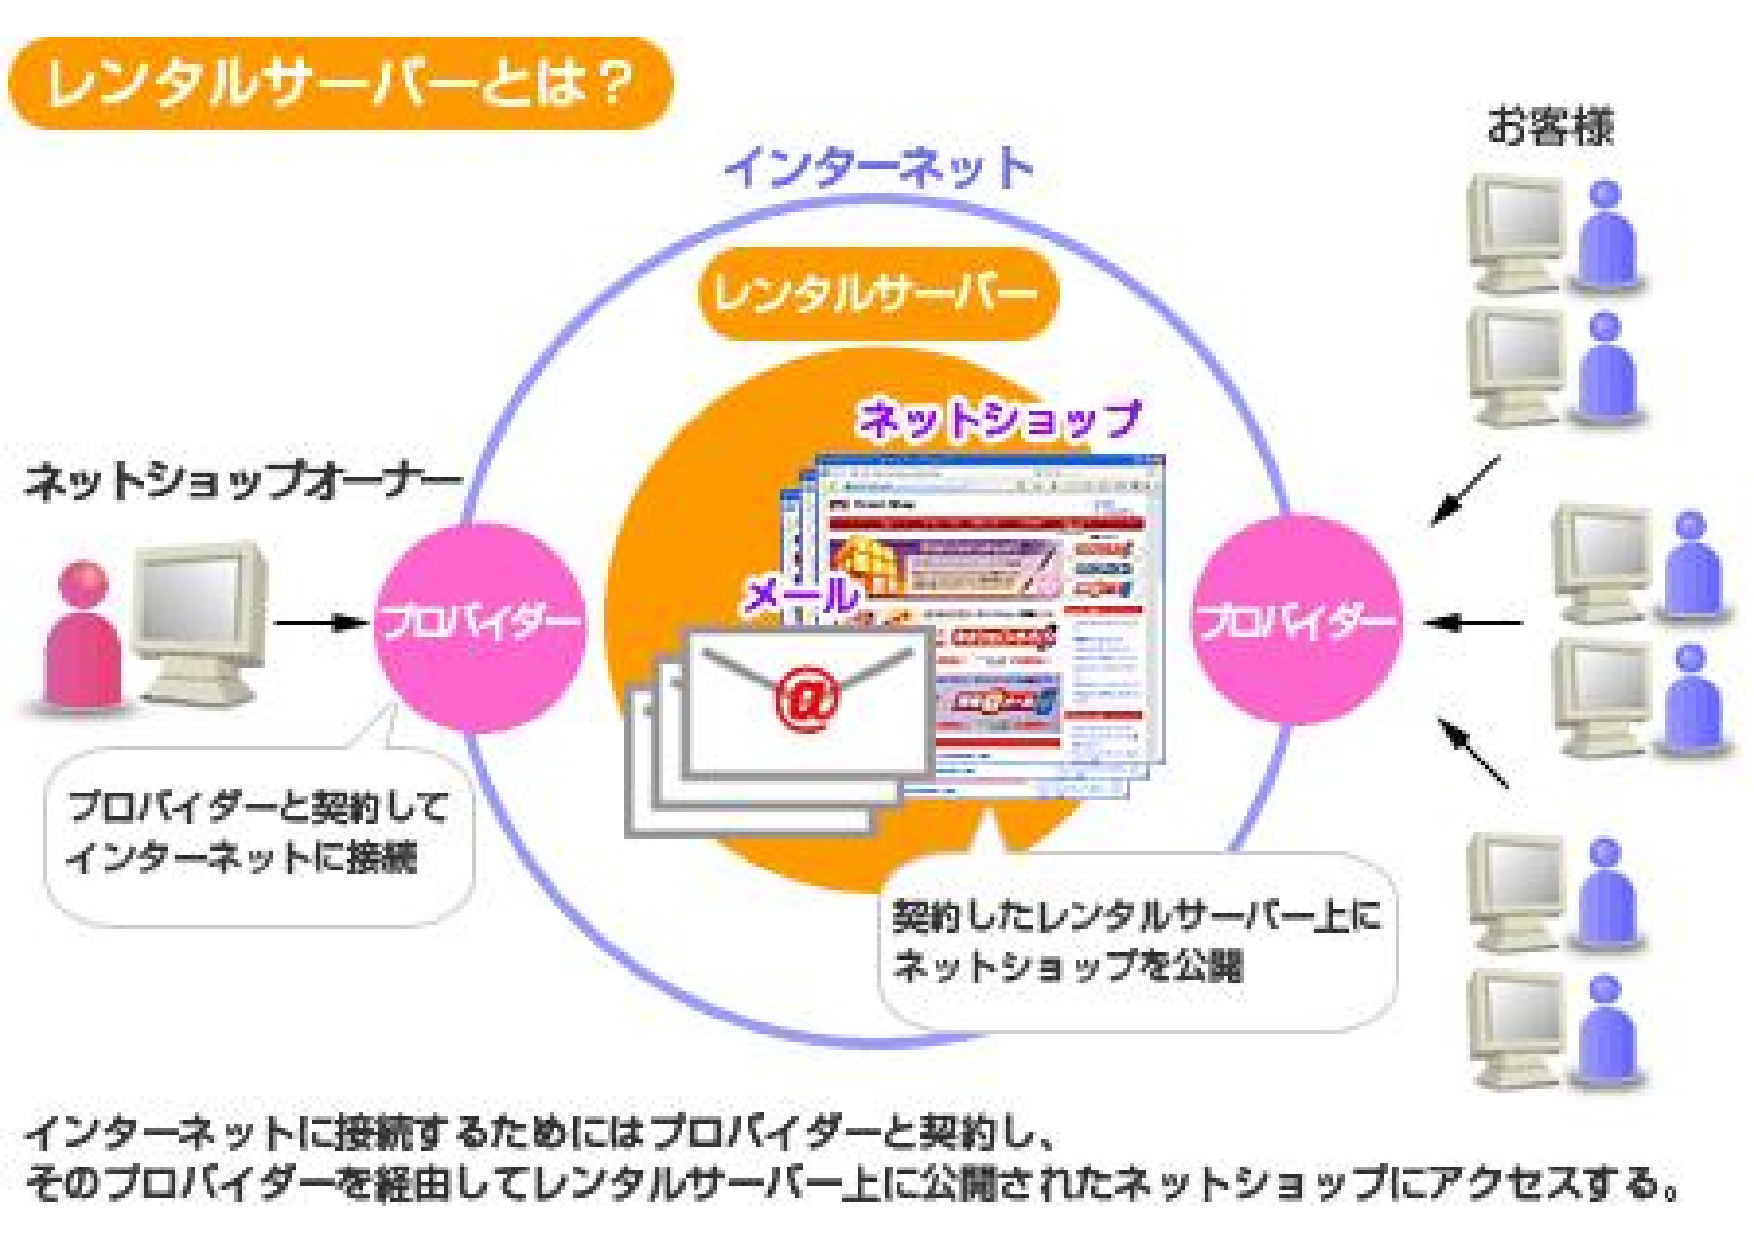
\includegraphics[width=8cm,clip]{rentalserver.pdf}
\caption{レンタルサーバーとは}
\label{rentalserver}

\end{figure} 

プロパイダーの中にはネット接続サービスだけでなく,ホームページを公開しているものもある.しかし,ショッピングカート機能がない場合が多い.

また,プロパイダー次第では,商用利用が禁止される,SSLに対応していないことがあるため,レンタルサーバーを利用するほうが安易に運用できる.

\begin{table}[htb]

\label{プロパイダーとレンタルサーバーの違い}
    \caption{プロパイダーとレンタルサーバーの違い}
\newlength{\providervsrentalserver}
\setlength{\providervsrentalserver}{0.7cm}
  \begin{center}

\begin{tabular}{|r|p{10em}|p{10em}|}
\hline



	種別 & プロパイダー経由 & レンタルサーバー  \\ \hline \hline
	\parbox[c][\providervsrentalserver][c]{0cm}{}
	ホームページ容量 & 10MB~300MB & 1GB~40GB \\
	\parbox[c][\providervsrentalserver][c]{0cm}{}
	独自ドメインの利用 & 可能 & 可能  \\
	\parbox[c][\providervsrentalserver][c]{0cm}{}
	SSL & 非対応 & 対応  \\
	\parbox[c][\providervsrentalserver][c]{0cm}{}
	メールアドレスの数 & 1 & 10~  \\
	\parbox[c][\providervsrentalserver][c]{0cm}{}
	商用利用 & 不可 & 可  \\
	\parbox[c][\providervsrentalserver][c]{0cm}{}
	データベースの利用 & 不可 & 可  \\
	\hline





	\end{tabular}
  \end{center}
 
\end{table}


\subsubsection{代金の回収方法}

ネットショップを始める場合,最初に導入したい決済方法は郵便振替,銀行振込,代金引換の3つである.1つではなく3つ用意するのは,お客さま視点で使いやすい方法を選択させるため.基本的に郵便振替や銀行振込は,ATMなどで振り込む手間がかかる.いっぽう代金引換は,そういった手間がない分,手数料が高いというデメリットがある.
「郵便振替」の場合は,郵便局で郵便振込口座を作り運転免許証などの本人確認できる証明書と印鑑があれば,誰でも簡単に開設できる.「銀行振込」も口座を開設するだけで開設できる.すでに使っている銀行口座があれば,それをそのまま振込先に指定することも可能だ.代金引換の場合は郵便局か宅配業者かどちらかを利用し郵便局は郵便振替同様,口座を開設すればすぐに利用でるが,宅配業者の場合は事前に契約を結ばなくてはならない.そのため,開業当初は郵便局のサービスを利用するほうが簡単である。

\begin{itemize}

 \item	郵便振替

\begin{itemize}
\setlength{\parskip}{3mm}

 \item	注文が全国各地からくるような商品の場合の設定方法.この場合の料金の設定は,たとえば発送元が東京都なら,都内での送料より高めにするのがよい.地方への送料を抑える分,都内での送料に上乗せするようにして全体的な送料のバランスを取りたい.お客さまに郵便振替用紙を送り,指定の郵便口座に入金してもらう方法.手数料はお客さまとショップ側とどちらが負担するかを事前に決めておく.入金確認は3,4日かかる.

\end{itemize}

 \item	銀行振込

\begin{itemize}
\setlength{\parskip}{3mm}
 \item	指定の金融機関の口座に入金してもらう方法で入金管理がしやすい.振込手数料が高いため,需要は低いように思えるが,銀行は全国各地にあるため意外と利用者は多い.

\end{itemize}

 \item	代金引換

\begin{itemize}
\setlength{\parskip}{3mm}

 \item	郵便局や宅配業者が商品を配達する際に,お客さまから購入代金を回収するという方法.代金は後日ショップの指定口座に振り込まれる.代引き手数料,振込手数料がかかる.

\end{itemize}

 \item	クレジットカード決済

\begin{itemize}
\setlength{\parskip}{3mm}

 \item	注文時にクレジットカード番号を入力してもらう方法.お客さまにとっては振込手数料もかからず便利だが,ショップ側が手数料を負担するため,安定した売上を見込めてから導入する.
\end{itemize}

 \item	コンビニエンスストア決済

\begin{itemize}
\setlength{\parskip}{3mm}
 \item	コンビニ用の払込票をお客さまに送り,最寄りのコンビニで商品代金を支払ってもらう方法.コンビニの多い都市部のお客さまには便利だが,コンビニの少ない地方のお客さまには不向き.

\end{itemize}
\end{itemize}


\subsubsection{ネットショッピングにおけるウイルスの危険性}

コンピュータ・ウイルスとは,システムを破壊したり,コンピュータ内からメールアドレスを抽出して被害を拡散するなど,人為的に作られた悪質なプログラムのことをいう.感染経路はメール,ホームページ,あるいは非合法なソフトがあたる。
例として,メールの受信をし用意,ウイルス付きメールを送り拡散するものもある.ウイルスに感染すると,被害者になると同時に他の人にもウイルスを拡散する加害者にもなってしまう.これは運営するにあたって,重大な問題となる.ウイルスによってショップの情報の消失,ウイルスに感染したメールをお客さまにまいては,築いてきたショップの信頼も崩れるだろう.

そのような事態を防ぐため,ネットショップを運営には最悪の事態に備え,万全なウイルス対策おこなう必要がある.
ウイルス対策ソフトを導入しても,日々新種ウイルスが生み出されているため必ず,更新する必要がある.添付ファイルにウイルスが感染している場合も考えられるので注意が必要である.





\subsection{ネットショッピングセンターに出店}

日本だけでなく,世界に浸透している複合型産業としてショッピングセンターがあがる.
技術の発展によりこのショッピングセンターをネットワーク上で運営することで,どこからでもアクセスさえ行えれば商品の回覧,購入が可能となった.
これを利用し個人でも出展が可能になり,商品単位での販売が行える.

\subsubsection{ショッピングセンターとは}

複数の小売店舗やサービス業,美容院,旅行代理店などの3次産業だけでなく,4次産業も組み込まれた商業施設である.

単独で運用される店舗と違い,顧客集客力が強く期待でき,それら客がくるまでの交通施設が整い駐車場や荷捌き施設も備わっているものが多い.

また,出店企業としては,貸し出しで営業を行うため建物に対する負担,劣化しないよう建物を維持する費用などが軽減できるため初期投資が軽減できる.

\begin{itemize}

 \item	ショッピングセンターの定義

日本におけるショッピングセンターの定義を日本ショッピングセンターが定めている.\cite{shopcenter}

\begin{itemize}
\setlength{\parskip}{3mm}


 \item	小売業の店舗面積は, $1500^{2}$ m以上であること.
 \item	キーテナントを除くテナントが10店舗以上含まれていること.
 \item	キーテナントがある場合、その面積がショッピングセンター面積の80\%程度を超えないこと。但し、その他テナントのうち小売業の店舗面積が  $1500^{2}$ m以上である場合には,この限りではない.
 \item	テナント会(商店会)等があり,広告宣伝,共同催事等の共同活動を行っていること.



\end{itemize}

 \item	世界のショッピングモールの歴史

2世紀のローマに建設された「トラヤヌスの市場」が人類史上初のショッピングモールとされる.

近代的なショッピングセンターとしては,1922年にアメリカ合衆国のカンザスシティで始まった不動産業者・J.C.Nicolsによる「カントリー・クラブ・プラザ」が最初のものといわれている.

その後の1950年前後からは車社会化と郊外住宅の発展を背景として,1948年にはオハイオ州コロンバスの不動産業者・Doncasterが開いた「タウン・アンド・カントリー・ショッピング・センター」,ワシントン州のシアトルでJ.B.Douglasが開いた「ノースゲート・ショッピング・センター」がショッピングセンターの原型となった.

1956年にDayton Hudsonがミネアポリス郊外に,最初の完全な共同店舗型のモール(下記参照)として「サウスデール・センター」を開いた.これは一個の街と呼べる巨大なもので,駐車場が広い上,ミネソタの厳しい冬でも快適に多数の店を回る買い物ができるため,ミネアポリス都市圏のみならず複数の州から買い物やイベントを楽しむ客が集まった.

1981年にカナダのアルバータ州エドモントンに開業した「ウェスト・エドモントン・モール」は、1998年に第4期工事が完成した段階で総床面積49万 $3000^{2}$ m,店舗数800でホテル,遊園地,水族館等を備え,年間2000万人の入場がある大規模なもので,世界最大のショッピングセンターとして『ギネスブック』に記載された.

 \item	日本のショッピングモールの歴史

1954年に米国施政下の沖縄県において「プラザハウスショッピングセンター」がオープンした.

1964年には「ダイエー庄内店」(現・グルメシティ庄内店)がオープンした.日本において初のショッピングセンターの実験をおこなった店舗であり,日本初のショッピングセンターでもある.1968年にはダイエー香里店(2005年閉店)がオープンした.日本初の本格的な郊外型ショッピングセンターが誕生した.これ以降,車社会化に対応したショッピングセンターが増加した.

1980年代以降,日本においても車社会化の進行で,郊外や農村部の幹線道路沿いの田畑を埋め立てや産業構造の変化に伴い閉鎖された大規模工場敷地跡等て広大な敷地を確保した大型ショッピングセンターの出店が数多く行われた.特に日米構造協議や規制緩和を経て,大規模小売店舗法が廃止され,大規模小売店舗立地法が制定された2000年以降,数と規模は大きく増えた.中でもモール型ショッピングセンターは1つの建物に数多くの専門店やアミューズメント店を揃えた大規模なもので,1日中滞在できる「時間消費型」の施設として,この時代の大型ショッピングセンターの代名詞ともなった.

 \item	種類

店舗面積などの規模によって,3種類に分類される

\begin{itemize}
\setlength{\parskip}{3mm}

 \item	リージョナル型ショッピングセンター

店舗面積 $4万^{2}$ m以上、半径8 - 25km程度の広域を基本商圏とする大型ショッピングセンター.総合スーパーや百貨店などを核店舗にした「1核1モール型」や,それらの核店舗に映画館や家電量販店など,集客性の高い大型専門店を加えて副核店舗へ集約し,相互の中間にモールを設置する「2核1モール型」を形成している施設などがある.専門分野の有名専門店,飲食店,サービス店,アミューズメント店など多種にわたる店舗が並び,その施設だけで1日買い物を楽しむ事を目的とした時間消費型の施設である.
リージョナル型よりさらに広範囲を商圏とする超大型の「スーパー・リージョナル型」は店舗面積 $10万^{2}$ 以上で基本商圏も8kmから40km程度まで設定している施設も存在する.

 \item	コミュニティ型ショッピングセンター

店舗面積1万 - $3万5000^{2}$ m程度、半径5 - 10km程度の地域を基本商圏とし,専門店が出店する中規模のショッピングセンター.日本ではこの形態が多く、専門店は最寄品やサービス店などが中心であった.こういった旧来型の店舗にモールの増築を行いリージョナル型に拡張された施設が増えている

 \item	ネイバーフッド型ショッピングセンター

店舗面積3000 - $3万5000^{2}$ m程度,半径5km程度の近隣地域を基本商圏とした小商圏型のショッピングセンターとしては比較的小規模な施設.食品スーパーやホームセンターなどを核店舗に比較的実用的な商品を扱う専門店で構成され身近な買い回りをターゲットとしている.比較的日常的に使われ来店頻度が高い.

\end{itemize}

 \item	建物について

\begin{itemize}
\setlength{\parskip}{3mm}

 \item	エンクローズドモール形式

施設自体が大きな1つの建物であり,通路が建物内にあるショッピングセンター.気候や天気に左右されないのが特徴で,大型のリージョナル型ショッピングセンターや,中型のコミュニティ型ショッピングセンターでよく見られる形態.
欠点としては建設コストが高いため出店リスクが高いことである.

 \item	オープンモール形式

店舗を結ぶ通路が屋外にあるタイプのショッピングセンター.店舗の入口の前に駐車場が広がり,駐車場から目的の店が近いため歩行距離が短くて済むものもある.店舗を結ぶ通路を屋外のペデストリアンデッキによって結ぶことで,買い回り性を上げているものもある.全体的に簡易な施設とすることで建設コストを抑制出来るため、中小事業者でも進出しやすいメリットがあり,ネイバーフッド型ショッピングセンターでよく見られる.

\end{itemize}

 \item	立地

\begin{itemize}
\setlength{\parskip}{3mm}

 \item	都市型

中心市街地など人口密集地に立地するショッピングセンター.日本では2000年に廃止された大店法の影響で大型店の出店が厳しく制限されていたため,大型店は中心市街地への出店が中心であった.中心市街地では車でのアクセスが悪い場所が多いため,鉄道や路線バスなど既存の公共交通機関利用での来客をメインに置いた施設が中心である.

 \item	郊外型

中心市街地から離れた郊外に立地するショッピングセンター.地価が高く土地交渉に時間の掛かる中心市街地への出店に比べて,郊外では割安で広大な土地が確保が可能であることから,2000年の大店法廃止以降に急激に増加した.駅から離れた施設の場合は自動車以外でのアクセス手段として最寄り駅や人口密集地から路線バスや無料送迎バスを運行している場合もある.

\end{itemize}

\end{itemize}

\subsection{ネットオークションの利用}

\subsubsection{ネットオークションとは}

1990年代以降,インターネットを通信媒体として利用したネットオークションサイトが登場し,一般の人でも手軽に出品や入札が可能だ.

ネットオークションはインターネット環境の整った国では一般的に利用され,国際取引も増加している.アメリカ・イギリス・オーストラリアなどの英語圏や,中国・台湾・シンガポールなど中国語圏での国際取引が活発で,国際宅配業者を利用したネットオークション取引が盛んである.
だが,アメリカはAmazon等の企業 - 個人間の電子商取引の充実に伴い,ネットオークションは当初の勢いを失っているという.消費者は,欲しいものであれば多少の値引きと引き替えにオークションに時間を取られることよりも,固定価格で手間をかけずに素早く購入できる買い物を望む傾向が強い.その結果,電子商取引において,ネットオークションよりも固定価格によるショッピングでの売買が伸びている.

日本ではYahoo!オークションが最大手のサイトとなっており,他に楽天オークションなどのオンラインショッピングサイトが独自のサービスを展開し利用者を集めている.ネットオークションサイト世界最大規模のeBay(イーベイ)も2001年に日本へ進出したが,先行していた日本独自のオンラインショッピングサイトにより,不振で翌2002年3月で日本から撤退した.eBayは2007年12月にYahoo!オークションと提携を行った.
KDDIがauオークションを提供し,NTTドコモもオークション事業に進出するなど、携帯電話・スマートフォンによるオークションも活発化している。

\begin{itemize}

 \item	ネットオークションのシステム

\begin{itemize}
\setlength{\parskip}{3mm}

 \item	出品

出品者が,商品の名称,状態,写真,開始額,終了日時等の出品に関する情報をオークションサイトのサーバにアップロードを行う.この出品情報に基づいてウェブページが生成され,オークションのウェブサイトに掲載され,オークションが開始される.

法律またはオークションの規定に違反した疑いがある場合,運営者によって出品が取り消されることがあり,出品時に支払った手数料が一切返金されない.

 \item	入札

入札者は,オークションサイトが備える検索機能によって希望する商品を検索し,購入希望額を指定して入札する.

商品の検索方法は,ジャンルごとに確立されたワードを登録することで検索が簡易的に行えるようになり,メールで告知されるなどの利便性が備わっている.

商品が掲載されたウェブページは随時更新されており,最新の状態を確認することができる.入札額は,第三者に公開されることが多いが非公開のシステムも存在する.
他の入札者により,自分の入札額を以上の入札が行われた場合には,再度入札を行い入札額を競り上げることが可能だ.最高入札額の更新を電子メールで通知する機能や,他者によって入札が行われた場合に,入札者があらかじめ指定しておいた限度額内で自動的に再入札を行う機能も一般的に備わっている.

 \item	落札

オークションの期間終了にともない.落札者,落札価格が確定され,商品のページで公表,入札者及び落札者の双方に電子メールで通知が行われる.取引相手の情報は商品のウェブページで入札者と落札者に公表される.
その後の入金や商品の発送などの取引は,基本的に当事者間で行われる。このため,メールアドレスを明かすことなく互いに連絡が可能な機能を利用することや金融機関や運送会社などと提携して,入金や商品発送を容易に行うことができるサービスが提供されている場合がある.

落札者と出品者が相手のそれまでのオークション上の行為の信頼度の参考にできるよう,システム上で出品者と落札者同士を評価する制度を備えることが多いが,出品・落札した商品名が他の参加者にも公開されるため,商品によってはプライバシーを侵害しかねない.

\end{itemize}

 \item	オークションで販売,購入のメリット,デメリット

\begin{itemize}
\setlength{\parskip}{3mm}

 \item	安価な値段で商品を手に入れることができる.

例:ブランド物のショルダーバック14万が5万で手に入る.

 \item	通常の商店では手に入らない物品が出品されている.現在の商店では在庫少ないもしくは存在しない場合でもオークションでは存在する可能性がある.

例:人気のドラマ,アニメ関連の在庫が少ない状態で販売されたストラップを手に入れたものがオークションで出品している.

 \item	商品の公開に手間がかかる.

例:WEBページに掲載する写真の撮影に数時間も要する.

 \item	出品者,購入者間でのトラブルの発生

例:個人対個人の取引のため,連絡が取れない場合泣き寝入りするケースがある.

 \item	商品購入までに時間がかかる.

例:落札時間を一週間に設定してしまったがゆえに引渡しに時間がかかった.

 \item	送料,振り込み手数料がかかる.

例:商品の値段が1000円にも関わらず送料で倍の2000円要した.

\end{itemize}

\end{itemize}

\subsection{ネットショップ作成専用ソフトの使用}

会員・ポイント機能も備えた本格的なネットショップを構築・運営することのできる、オールインワン・ネットショップ構築ソフトである.
ホームページさえ初めて作る方でも簡単にネットショップが作成できるように設計されている.

認知が広いものでいえばネットショップオーナーなどがあがる.

\subsubsection{ネットショップ作成専用ソフトで行える大まかな内容}

\begin{itemize}

 \item	商品管理

\begin{itemize}
\setlength{\parskip}{3mm}

 \item	フォルダやファイルを作る動作で商品カテゴリを作成し,商品の情報,画像,説明文などを入力して商品を登録することができる.

この商品管理で作成した商品カテゴリのツリー構造や商品の情報は,自動的に作成される商品ページに反映される.

 \item	ネットショップとリアルタイムに連動した在庫管理が可能

商品毎の在庫数は,注文数に応じて自動的に減算される.在庫が0になった商品はショップページで自動的に「在庫なし」の表示に切り替わり,注文を受け付けなくなるので,在庫切れの商品の注文を受け付けてしまうトラブルを未然に防ぐことができる.

\end{itemize}

 \item	ページデザイン

\begin{itemize}
\setlength{\parskip}{3mm}

 \item	ドラッグ&ドロップで自由にレイアウト可能

各ページの構成は,「モジュール」と呼ばれるものをドラッグ&ドロップで自由にレイアウトすることによって作成できる.
モジュールには,「メインメニュー」や「検索ボックス」など,ネットショップでよく使われる要素や機能があらかじめ用意されているものと,HTMLエディタによって全く自由に作成することができるものがある.

 \item	SEO(検索エンジン最適化)に対応したページを自動生成

SEO対策の基本として,各ページの<TITLE>タグ(ページタイトル)にキーワードを設定しておくことが非常に有効である.

「タイトル自動設定」で設定したルールに従い,ページ毎に商品名,カテゴリ名を自動的に入れ込むことができる.

\end{itemize}

 \item	受注管理

\begin{itemize}
\setlength{\parskip}{3mm}

 \item	「仕分け箱」に自動で受注の状態に応じて仕分け

サーバー上のショッピングカートで受注したデータは,メールを受信するようにサーバーから受注データを取り込み.仕分けフォルダ形式のインターフェースで管理できる.

 \item	受注検索機能

受注検索機能は,文字列による条件,数値による条件,日付による条件などの複数の条件を組み合わせて目的のデータの検索が可能である.

\end{itemize}	

\end{itemize}


\subsection{無料レンタルサービスの使用}

無料のレンタル・ネットショップがネット上には存在する.

一般的には有料のサービスが,無料で提供されている.しかし,無料であるが故の問題点も抱えている.


\subsubsection{レンタルサービスを使用するメリットとデメリット}

\begin{itemize}

 \item	費用がかからない

当然ながら無料であるため,本人が運用管理する人件費程度しか費用がかさむことがない.

 \item	ドメインオーソリティが高い

ドメインオーソリティはドメインの信頼度を意味する.ドメインオーソリティが高ければ,検索サイトでの検索結果が有利に働く可能性がある.

 \item	商品データさえあれば,ネットショップが開店できる.

在庫管理機能や顧客管理機能,携帯ショッピングにも対応,カード決済にコンビニ決済,有料サービスと遜色ない充実した内容が整っているものが多い.

 \item	無料サービスであるが故に収入が不安定であり,サービスの継続が不可になりえる可能性が高い.

サービスが終了してしまえば,閉鎖もしくは移転を行わなければいけないため,バックアップは必要不可欠なものとなる.

 \item	広告が挿入される.

無料サーバーのため,広告が自動で挿入され,削除ができないので外見のマイナスに繋がることもある.

 \item	検索結果に同一サービス(ドメイン)から数個しか表示されない

例として,10万のアカウント(ユーザー),100万ページを持つAという無料レンタルサーバーがあり,「副業」で検索する.検索結果には、Aのページからは数個しか表示されない.

つまり,100万ページから選ばれた2,3ページだけが検索結果に表示され,残りの99万9997ページは「存在しない」ということになるため,検索結果で著しく不利となる.

 \item	PHPやCGIやデータベースなどが使えないものが多い

WordPressやMovable TypeなどのツールやCGIを使ったサイト構築ツールなどを使用できない.
無料レンタルサーバーでは,htmlを使ったホームページが主流になる.無料ブログではブログを作れるが,PHPやCGIなどは使えない.

 \item	独自ドメインを使用できない

新規に取得した独自ドメインを無料レンタルサーバー上で使うことができない.

 \item	メールアカウントがない

独自ドメインを使える場合はオリジナルのメールアドレスを持つことが可能である.しかし,無料レンタルサーバーでは,メールアドレスは提供されていないので,別途メールアドレスを持つ必要がある.


\end{itemize}



\subsection{レンタルカートの使用}

ネットショップの開設に必要なものを大きく分けると,ショップページ,ショッピングカート,管理システムの3つに分けられる.

このうちショップページを自分でhtmlを使用して作成してショッピングカート,管理システムをレンタルする方法である.

\subsubsection{レンタルカートの使い方}

店舗ページを作った上で商品ページで「カートに入れる」ボタンを設置してそれをクリックすることでレンタルカートと連動させる.

これを行うことで,商品データがレンタルカートに送られ,計算やメール送信処理を行う.

レンタルカート内には,「商品ページに戻る」ボタンや「HOMEに戻る」というボタンがあるが,これらにオリジナルで作ったお店ページのリンクを入れることで,双方向を行き来可能となる.


\subsection{自作}

レンタルショップを利用することが当然になり手間もかからないため現在ではそれを利用するのが一般的であるが,自作するのが一般的であった時期もあった.

html,CGI,JavaScript,SSI,PHPなどの言語を駆使し,自身の能力でサイトを構築することである.


\subsubsection{自作で作成する場合の手順}

\begin{enumerate}

 \item	有料でドメイン,サーバーの取得

 \item	ネットショップに必要なページの作成

\begin{enumerate}
\setlength{\parskip}{3mm}

 \item	トップページ

 \item	商品ページ

 \item	特定商取引法のページ

など.

\end{enumerate}

 \item	トップページのデザインやレイアウト

 \item	商品ページの作成

 \item	商品データをCSVファイルなどに

 \item	アップロード

\end{enumerate}


\subsection{オープンソースでの作成}

オープンソースとは無料で配られているサーバ・アプリケーションに該当する.ネットショップ機能用のもあれば,ブログやSNS,通常のホームページのものなどの多岐に渡る.骨組みが作られているので完成させるには手間がそこまでかからない.

\subsubsection{オープンソースの種類}

ネットショップ用のオープンソースは、主に3種類ある.osCommerce,zencart,最も新しいのがEC CUBEである.


いずれのオープンソースも,専用サイトからダウンロードしてサーバーにアップロードして使用する.サーバーにインストールするだけで使えるが,無味乾燥なデザインとなるので,カスタマイズを行う.


アップロード時はzipなどの圧縮ファイル形式なので,ローカル上で解凍してFTPソフトを使って転送する.あるいは,「tar.gz」形式の圧縮ファイルなら,圧縮ファイルのままWindSCPなどのクライアントソフトでサーバに転送し,サーバー上で解凍展開することも可能である.

オープンソースを扱うには,サーバーの仕組みの理解,各種ソフトの扱い,HTML,CSS,CGI,PHP,Java Scriptなどの知識は必須である.

オープンソースそのものは無料だが,ソースを動かすサーバー代とHTPPSプロトコルのための独自SSLの費用,クレジットカードを導入する場合はその手数料など,レンタルネットショップを借りるのに比べて費用的メリットはさほど大きくないのが実情である.

\begin{table}[htb]

\label{クレジットカード導入に当たる手数料の比較}
    \caption{クレジットカード導入に当たる手数料の比較}
\setlength{\providervsrentalserver}{0.7cm}
  \begin{center}

\begin{tabular}{|r|p{15em}|p{15em}|}
\hline



	サービス名 & EC CUBE(オープンソース) & ショップサーブ(レンタル・ネットショップ)  \\ \hline \hline
	\parbox[c][\providervsrentalserver][c]{0cm}{}
	初期費用 & 5万円~ & 0円 \\
	\parbox[c][\providervsrentalserver][c]{0cm}{}
	カード手数料 & 3.5\%~ & 3.675\%~  \\
	\hline


	\end{tabular}
  \end{center}
 
\end{table}

\subsection{ブログで作成}

ブログをネットショップとして使う方法もある.
その場合,確認したいのが,そのブログサービスが商用利用を許可しているか否かである.商用利用とは,各種商品の販売やアフィリエイトなど,報酬目当てであるかどうかということ.

商用利用が可能な代表的なブログサービスとしては,Ameba blogやのSEESAA BLOGが該当する.ただし,公序良俗に反するような内容のと判断された場合は利用停止措置も辞さないと公表している場合もある.

ブログを使って販売する手法は、大きく分けて4つのタイプが存在する.

\begin{itemize}

 \item	メール受注

\begin{itemize}
\setlength{\parskip}{3mm}

 \item	最も簡単な手法であるメール受注.商品の記事をあげると同時に,受注用メールアドレスを公開しておき,「必要な人はメールにてご注文ください」とする方法.ブログ記事を作成できるスキルがあれば,即日販売開始ができるメリットがある.

\end{itemize}

 \item	フォーム受注

\begin{itemize}
\setlength{\parskip}{3mm}

 \item	受注フォームではないが,Googleドライブを使用しアンケートフォームが作成できる.Googleドライブを使えば,受注フォームが簡単に作成可能である.記事を上げると同時に,フォームのリンクを案内,常時表示される箇所に,「ご注文はこちらまで」と受注フォームに飛ぶように設定するなどの方法がある.

\end{itemize}

 \item	ショッピングカート受注

\begin{itemize}
\setlength{\parskip}{3mm}

 \item	商品記事をあげると同時に,カートボタンを配置し,必要な人ばカートボタンを押すことで,通販サイトの買い物ステップと同じように手続きを進める方法.自動的に送料が加算され,注文完了と同時に確認メールが送信など,一般的なショッピングサイト並の機能を備えている.

\end{itemize}

 \item	CMSカスタマイズ

\begin{itemize}
\setlength{\parskip}{3mm}

 \item	ブログCMSである,WordpressやMovable Typeを,ブログシステムからショッピングシステムへと改造してしまう方法.完成にたどり着いてもメンテナンスの手間は常時発生する.

\end{itemize}	

\end{itemize}


\subsection{メール受注のネットショップ作成}

ショッピングカートがない場合でも販売可能である.商品を並べ,「欲しい人はメールしてください」と書くだけある.このような方法で注文を受け付けている店も存在した.

ショッピングカートのメリットは複数の商品を同時に購入できる点である.複数のアイテムを扱っていないのならショッピングカートは使わなくてもよいということになる.例としてメールフォームなどが該当する.

\begin{figure}[htbp]

\centering
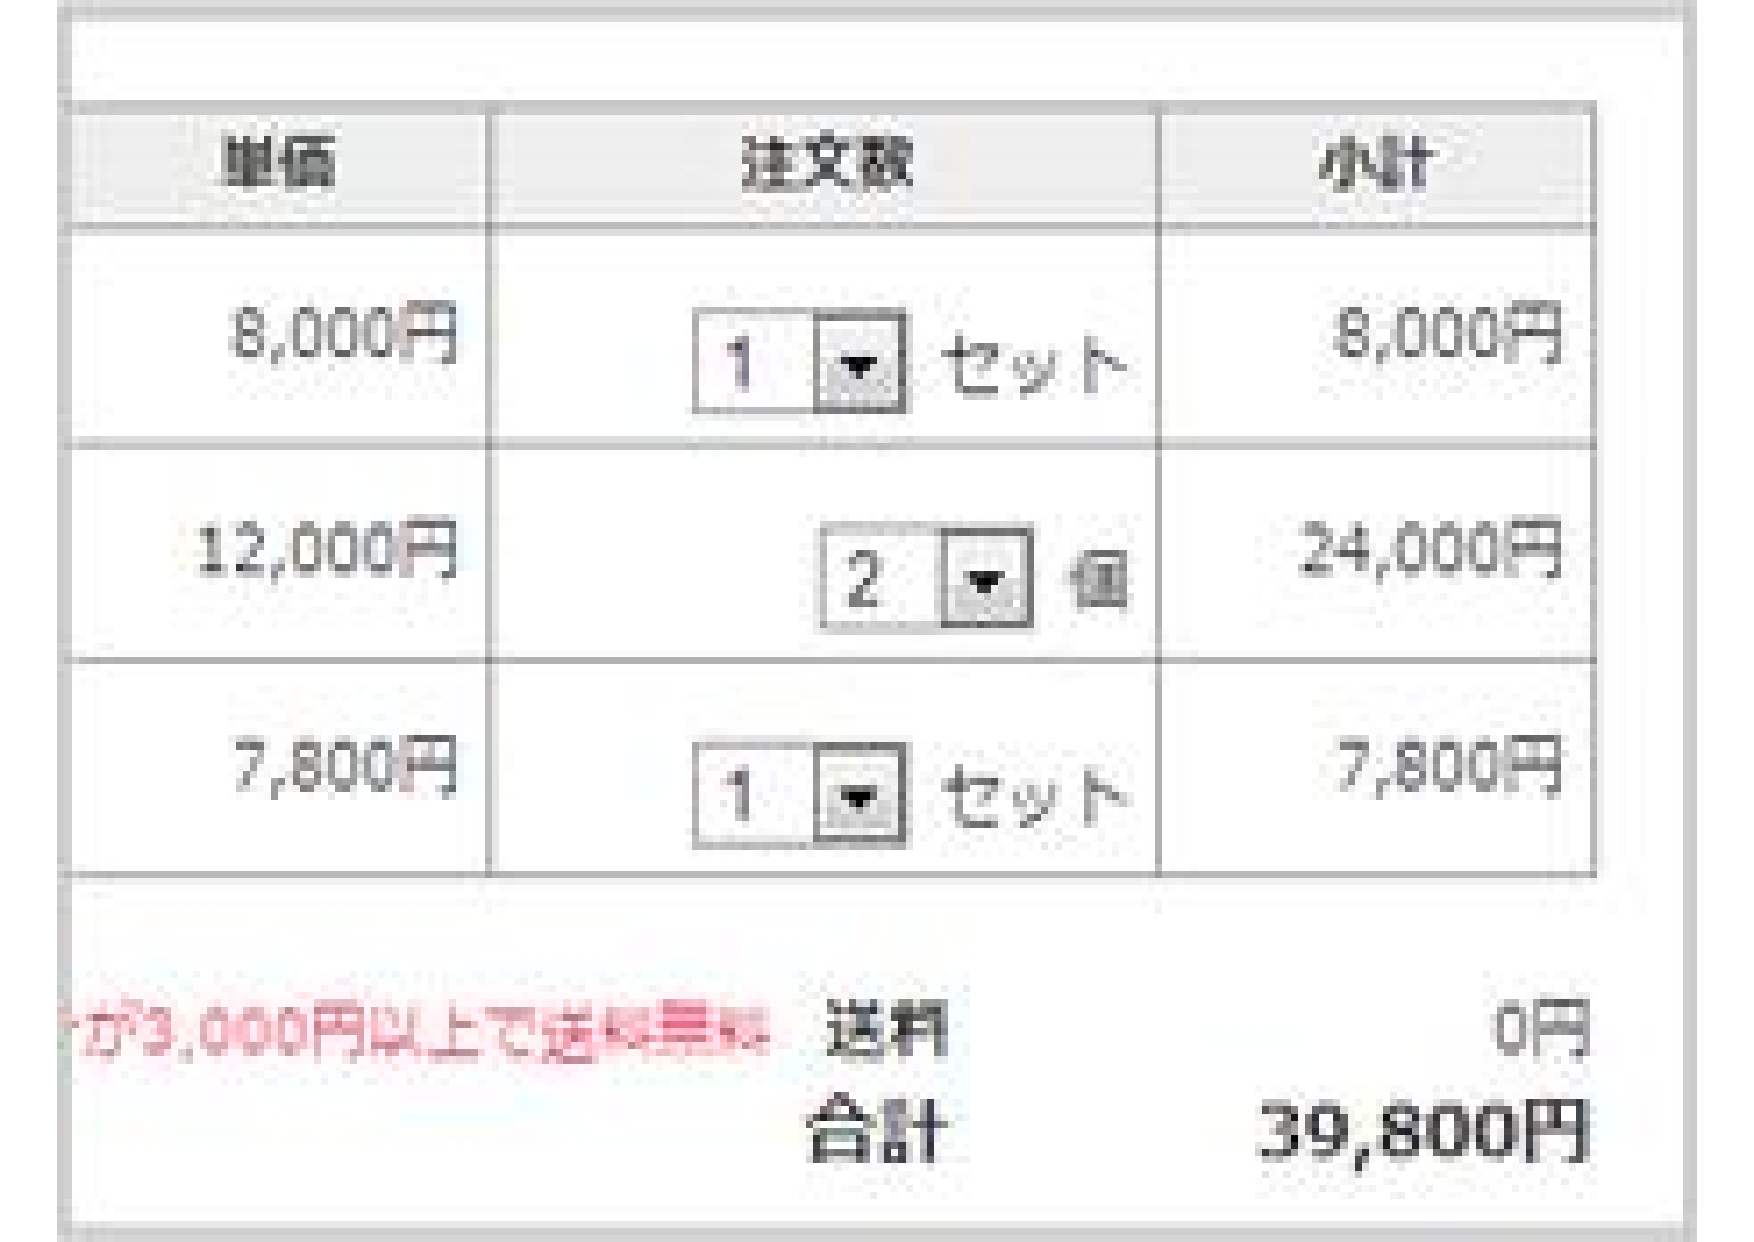
\includegraphics[width=8cm,clip]{fromsample.pdf}
\caption{注文フォームサンプル}
\label{fromsample}

\end{figure} 



\subsection{業者によるオーダーメード}

住宅を購入する場合,建売住宅を購入する方法と,設計図から始める注文住宅があるように,業者に依頼すれば,ネットショップを設計からスタートしオーダーメードで作ってもらうことも可能である.

趣向に合わせたデザイン,システムなど希望通りのお店作りが可能である.

業者に依頼する場合,依頼者がどんなショッピングサイトを作って欲しいのか,コンセプトから仕様までを事細かく説明できる必要がある.
業者に質問を受けた際にも,完璧に答える必要があり,的確に指示も出せる必要がある.



\section{2015年10月時点でのオンラインショッピングサイトのアクセス数}

下記に2015年10月時点でのオンラインショッピングサイトのアクセス数を50位までランキング化した表を記す.

\clearpage


\begin{table}[htb]

\label{週間アクセス数ランキング}
    \caption{週間アクセス数ランキング}
\newlength{\myranking}
\setlength{\myranking}{0.7cm}
  \begin{center}

\begin{tabular}{|r|r|p{30em}|}
\hline



	順位 & アクセス数(回) & サイト名  \\ \hline \hline
	\parbox[c][\myranking][c]{0cm}{}
	1 & 263262 & 価格.com \\
	\parbox[c][\myranking][c]{0cm}{}
	2 & 61522 & Amazon.co.jp  \\
	\parbox[c][\myranking][c]{0cm}{}
	3 & 54200 & 楽天市場  \\
	\parbox[c][\myranking][c]{0cm}{}
	4 & 37225 & Yahoo!オークション  \\
	\parbox[c][\myranking][c]{0cm}{}
	5 & 7742 & 楽天オークション  \\
	\hline
	\parbox[c][\myranking][c]{0cm}{}
	6 & 7200 & ZOZOTOWN - 日本最大級のアパレル系ショッピングサイト  \\
	\parbox[c][\myranking][c]{0cm}{}
	7 & 6782 & Yahoo!ショッピング  \\
	\parbox[c][\myranking][c]{0cm}{}
	8 & 6687 & Oisix(おいしっくす)  \\
	\parbox[c][\myranking][c]{0cm}{}
	9 & 5891 & eBay公認 セカイモン  \\
	\parbox[c][\myranking][c]{0cm}{}
	10 & 5558 & 高島屋オンラインストア  \\
	\hline
	\parbox[c][\myranking][c]{0cm}{}
	11 & 5342 & 北海道わけあり市場  \\
	\parbox[c][\myranking][c]{0cm}{}
	12 & 5147 & ナニデル.com  \\
	\parbox[c][\myranking][c]{0cm}{}
	13 & 4761 & おとりよせネット   \\
	\parbox[c][\myranking][c]{0cm}{}
	14 & 3964 & ラーメン通販・ラーメン通ドットコム  \\
	\parbox[c][\myranking][c]{0cm}{}
	15 & 3397 & 宅麺.com  \\
	\hline
	\parbox[c][\myranking][c]{0cm}{}
	16 & 3334 & ドラぷらショッピング \\
	\parbox[c][\myranking][c]{0cm}{}
	17 & 2866 & WANTED AUCTION !   \\
	\parbox[c][\myranking][c]{0cm}{}
	18 & 2775 & iTunes Store(アイチューンズ・ストア)  \\  
	\parbox[c][\myranking][c]{0cm}{}
	19 & 1715 &便秘解消へ オリゴ糖ドットコム \\
	\parbox[c][\myranking][c]{0cm}{}
	20 & 1715 & みんなのケータイ・オークション「モバオク」 \\
	\hline
	\parbox[c][\myranking][c]{0cm}{}
	21 & 1647 &グーオク  \\

	\parbox[c][\myranking][c]{0cm}{}
	22 & 1216 &比較.com \\

	\parbox[c][\myranking][c]{0cm}{}
	23 & 1075 &【楽天市場】みかん | 週間売れ筋人気ランキング \\

	\parbox[c][\myranking][c]{0cm}{}
	24 & 1074 &バイク用品通販のWebike(ウェビック) \\

	\parbox[c][\myranking][c]{0cm}{}
	25 & 1010 &通販生活 \\
	\hline





	\end{tabular}
  \end{center}
 
\end{table}








\clearpage









\begin{table}[htb]

\setlength{\myranking}{0.7cm}
  \begin{center}

\begin{tabular}{|r|r|p{30em}|}
\hline


	順位 & アクセス数(回) & サイト名  \\ \hline \hline


	\parbox[c][\myranking][c]{0cm}{}
	26 & 990 &送料の虎 - 宅配便・郵便・引越しの料金比較  \\

	\parbox[c][\myranking][c]{0cm}{}
	27 & 956 &無印良品ネットストア  \\

	\parbox[c][\myranking][c]{0cm}{}
	28 & 945 &ほぼ日手帳  \\

	\parbox[c][\myranking][c]{0cm}{}
	29 & 924 & DMM.com いろいろレンタル \\

	\parbox[c][\myranking][c]{0cm}{}
	30 & 924 & 日テレ7 \\
	\hline
	\parbox[c][\myranking][c]{0cm}{}
	31 & 894 &ネットプライス \\

	\parbox[c][\myranking][c]{0cm}{}
	32 & 884 & ペルメゾンネット 防寒グッズ \\

	\parbox[c][\myranking][c]{0cm}{}
	33 & 878 &TWO TOP \\

	\parbox[c][\myranking][c]{0cm}{}
	34 & 858 & 世界最大オークションeBay の日本向け公認サイト セカイモン \\

	\parbox[c][\myranking][c]{0cm}{}
	35 & 846 & オンライン書店【Honto】 \\
	\hline
	\parbox[c][\myranking][c]{0cm}{}
	36 & 831 & Sony ストア \\

	\parbox[c][\myranking][c]{0cm}{}
	37 & 817 & 三省堂書店 \\

	\parbox[c][\myranking][c]{0cm}{}
	38 & 816 & ノジマオンライン \\

	\parbox[c][\myranking][c]{0cm}{}
	39 & 781 & 激安!家電のタンタンショップ \\

	\parbox[c][\myranking][c]{0cm}{}
	40 & 767 & DMM.com 通販 \\
	\hline
	\parbox[c][\myranking][c]{0cm}{}
	41 & 745 & ソフマップ.com \\

	\parbox[c][\myranking][c]{0cm}{}
	42 & 745 &クロネコヤマトのブックサービス \\

	\parbox[c][\myranking][c]{0cm}{}
	43 & 733 & BOOK TOWN じんぼう \\

	\parbox[c][\myranking][c]{0cm}{}
	44 & 669 & 時計屋ネット - 時計ベルトの専門店 \\

	\parbox[c][\myranking][c]{0cm}{}
	45 & 656 & モンベル オンラインショップ  \\
	\hline
	\parbox[c][\myranking][c]{0cm}{}
	46 & 643 & 株式会社オートウェイ \\

	\parbox[c][\myranking][c]{0cm}{}
	47 & 621 & 楽天市場のバレンタイン特集 \\

	\parbox[c][\myranking][c]{0cm}{}
	48 & 607 & ダイヤテック・オンラインショップ \\

	\parbox[c][\myranking][c]{0cm}{}
	49 & 605 & オルビス クリアシリーズ \\

	\parbox[c][\myranking][c]{0cm}{}
	50 & 597 &こたつ通販【家具屋赤や こたつ館】 \\
	\hline


	\end{tabular}
  \end{center}
 


\end{table}


\subsubsection{ランキングから考察するオンラインショッピングの環境状態}

このようにオンラインショッピングといえど,50を上回るほどの十分な数があることが分かる.

勿論,ランキングとしてアクセス数の高いもののみを表記しただけなので実際にはこれ以上にオンラインショッピングを行える環境が整っていると言える.






\newpage






\subsection{アクセス数と資本金による企業規模の判断}


\begin{table}[htb]
\label{アクセス数上位4位以上の資本金}
    \caption{アクセス数上位4位以上の資本金}

\newlength{\shihonkin}
\setlength{\shihonkin}{0.7cm}
  \begin{center}

\begin{tabular}{|r|p{12em}|p{20em}|}

	\hline
	アクセス数順位 & 企業名 & 資本金  \\
	\hline
	\parbox[c][\shihonkin][c]{0cm}{}
	1位 & 株式会社カカクコム & 9億1598万4千円,(2015年3月31日時点)  \\
	\hline
	\parbox[c][\shihonkin][c]{0cm}{}
	2位 & Amazon.com, Inc. & 9824億900万円,(2012年12月31日時点)  \\
	\hline
	\parbox[c][\shihonkin][c]{0cm}{}
	3位 & 楽天株式会社 & 1116億100万円,(2014年12月31日時点)  \\
	\hline
	\parbox[c][\shihonkin][c]{0cm}{}
	4位 & ヤフー株式会社 & 83億200万円,(2015年6月時点)  \\
	\hline
    \end{tabular}
  \end{center}
\end{table}


\subsubsection{資本金から考察する企業規模}

上記の図からわかるように,アクセス上位企業でありながらにして資本金に大きな差があることが伺える.

資本金を基準に企業規模を図る場合,Amazon,楽天,Yahoo!,が大手ショッピングサイトと位置づけられるだろう.

\subsubsection{株式会社カカクコムについて}
アクセス数が1位である株式会社カカクコムは,回覧者に向けてメーカーごとに商品の価格の差異を提供する情報サイトである.

株式会社カカクコムのサイト自体にはショッピングサイトとしての機能は備わってなく,販売する企業のサイトに誘導し,そこで購入を行うことになる.

そのため,株式会社カカクコムに利益が向かうことが少なく資本金に大きな差があると考えられる.





\newpage






\section{オンラインショッピングサイトの歴史}

大手企業として表記した「楽天,Yahoo!,Amazon」等を中心にオンラインショッピングサイトとしての歴史を下記に記す.

1995年以前にもオンラインショッピングサイトを運営する試みが行われたことはあるが企業名が判明せずそれ以降の記載となる.


\begin{table}[htb]

\label{オンラインショッピングサイトの歴史}
  \begin{center}
    \caption{オンラインショッピングサイトの歴史}
\newlength{\myheight}
\setlength{\myheight}{0.7cm}

\begin{tabular}{|r||l|}
\hline

	年度 & 内容  \\ \hline \hline
	\parbox[c][\myheight][c]{0cm}{}
	1995 & Amazonがサービス開始  \\
	\hline
	\parbox[c][\myheight][c]{0cm}{}
	1997 & AmazonがNASDAQに上場,1株18ドル  \\
	\parbox[c][\myheight][c]{0cm}{}
	1997 & 楽天がサービス開始  \\
	\hline
	\parbox[c][\myheight][c]{0cm}{}
	1999 & zapposがサービス開始  \\
	\parbox[c][\myheight][c]{0cm}{}
	1999 & Yahoo!ショッピングがサービス開始  \\
	\parbox[c][\myheight][c]{0cm}{}
	1999 & Yahoo!オークションがサービス開始  \\
	\parbox[c][\myheight][c]{0cm}{}
	1999 & 楽天市場フリマオークションがサービス開始  \\
	\hline
	\parbox[c][\myheight][c]{0cm}{}
	2000 & 携帯電話向けYahoo!モバイルサービス開始  \\
	\parbox[c][\myheight][c]{0cm}{}
	2000 & 楽天市場共同購入サービス開始  \\
	\parbox[c][\myheight][c]{0cm}{}
	2000 & ケータイ版楽天市場サービス開始  \\
	\parbox[c][\myheight][c]{0cm}{}
	2000 & 日本版サイトAmazon.co.jpがサービス開始  \\
	\parbox[c][\myheight][c]{0cm}{}
	2000 & ネットバブル崩壊  \\
	\hline
	\parbox[c][\myheight][c]{0cm}{}
	2001 & Yahoo!オークション有料化  \\
	\parbox[c][\myheight][c]{0cm}{}
	2001 & Amazonアソシエイトプログラム開始  \\
	\hline
	\parbox[c][\myheight][c]{0cm}{}
	2002 & Google ショッピング開始  \\
	\hline
	\parbox[c][\myheight][c]{0cm}{}
	2003 & 楽天市場スーパーアフィリエイト開始  \\
	\hline
	\parbox[c][\myheight][c]{0cm}{}
	2004 & mixiがサービス開始   \\
	\parbox[c][\myheight][c]{0cm}{}
	2004 & 楽天市場オークション開始  \\  \hline



    \end{tabular}
  \end{center}
\end{table}









\newpage








\section{オンラインショッピングサイトにおける利点と欠点}

\subsection{購入者から見た利点と欠点}

\begin{itemize}
 \item	利点
\begin{itemize}
\setlength{\parskip}{3mm}
 \item	商品を探す場合,検索機能に加え,自分が重要視する項目でソートを行える.
 \item	商品として関連がないものの支払いや配送をまとめて行えるため,手間がかからない.
 \item	商品の種類が多岐に渡り購入できるため,店舗ごとに商品を探す必要がない.

\end{itemize}


 \item	欠点
\begin{itemize}
\setlength{\parskip}{3mm}
 \item	実際に触れて確かめることができない.
 \item	購入が決定してから配送し,自宅に届ける必要があるため,実際に手元に来るまで時間がかかる
 \item	オンラインショップを利用して販売することで手数料という販売経費が生まれたことで販売価格が上昇し,消費者が負担する可能性がある.

\end{itemize}

\end{itemize}



\subsection{販売者から見た利点と欠点}

\begin{itemize}
 \item	利点
\begin{itemize}
\setlength{\parskip}{3mm}
 \item	購入された商品の支払いや配送をまとめて行える.
 \item	商品の種類が多岐に渡るため,サイトとしての認知が高まり,客を集めやすい.
 \item	一定数顧客が存在するWebサイトに参入することにより,自社運用Webサイトよりも収益が見込める可能性がある.
 \item	商品を出す企業側は自分たちでWebサイトの運用を行わないので,コストを抑えることが出来る.

\end{itemize}


 \item	欠点
\begin{itemize}
\setlength{\parskip}{3mm}
 \item	同業他者との差を出しづらく,特徴が分かりづらい
 \item	売上の一部を,モール運営者に手数料を支払わなくてはならない.
 \item	オンラインショップを利用して販売することで手数料という販売経費が生まれたことで販売原価が上昇する
	
\end{itemize}

\end{itemize}








\chapter{Amazonについて}


\section{Amazonとは}

アメリカ合衆国・ワシントン州シアトルに本拠を構えている.
事業内容はWorld Wide Web上仮想店舗の運営であり,インターネット上の商取引の分野で初めて成功した企業の一つである.
2014年時点でアメリカ国外では,13カ国 (表\ref{Amazon国外サイト運営状況})でサイトを運営している.



\begin{table}[htb]
\label{Amazon国外サイト運営状況}
  \begin{center}
    \caption{Amazon国外サイト運営状況}


\begin{tabular}{|r|p{15em}|}

	\hline
	場所名 & ドメイン  \\
	\hline
	イギリス & amazon.co.uk  \\
	\hline
	フランス & amazon.fr  \\
	\hline
	ドイツ & amazon.de  \\
	\hline
	カナダ & amazon.ca  \\
	\hline
	日本 & amazon.co.jp  \\
	\hline
	中国 & amazon.cn  \\
	\hline
	イタリア & amazon.it  \\
	\hline
	スペイン & amazon.es  \\
	\hline
	ブラジル & amazon.com.br  \\
	\hline
	インド & amazon.in  \\
	\hline
	メキシコ & amazon.com.mx  \\
	\hline
	オーストラリア & amazon.com.au  \\
	\hline
	オランダ & amazon.nl  \\
	\hline
    \end{tabular}
  \end{center}
\end{table}








\newpage









\section{Amazonでの商品の購入方法}

ネット上におけるショッピングの仕方と現地でのショッピングには差がある

そこで,本項目ではオンラインショッピングにおける業界最大手であるAmazonでの商品の購入手順を解説していく.

\subsection{商品の購入方法}

\begin{enumerate}
 \item インターネット上のサイトの「www.amazon.co.jp」へ移動し,Amazonのページを表示する.
 \item Amazonのページ(\ref{Amazonでの購入解説})で赤丸の印の部分をクリックし購入したいワードを入力することで,商品が検索できる.また,青丸の印の部分をクリックするとカテゴリを選べるので,その状態で検索を行えばカテゴリごとに絞込みが行える.



%図の挿入
\begin{figure}[htb]
\centering
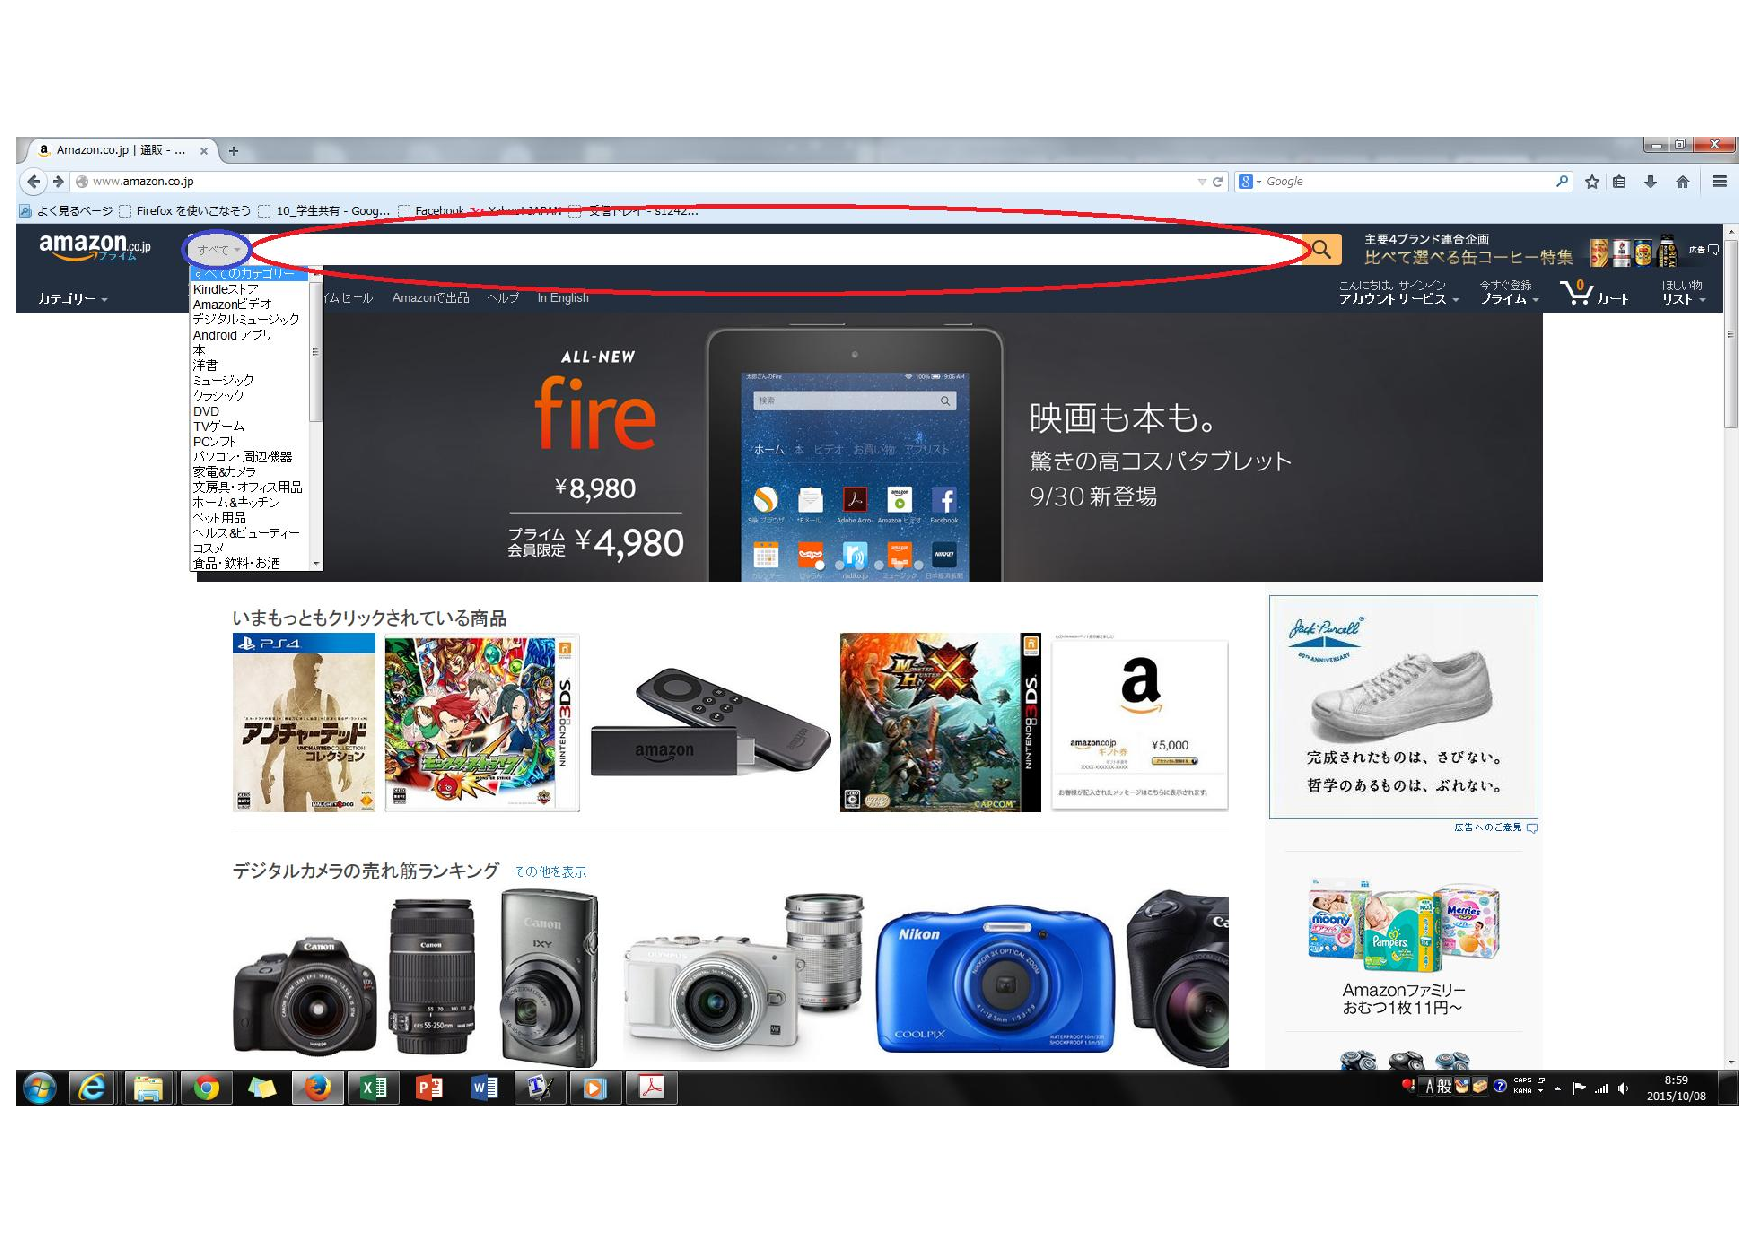
\includegraphics[width=10cm]{kensakuhouhou.pdf}
\caption{Amazonでの購入解説}
\label{Amazonでの購入解説}
\end{figure}

 \item 購入したい商品が決定した場合商品のページ(\ref{Amazonでの購入解説2})で,赤丸の印の部分をクリックし「カートに入れる」を選択することで次の画面に移動する.

\clearpage



%図の挿入
\begin{figure}[htb]
\centering
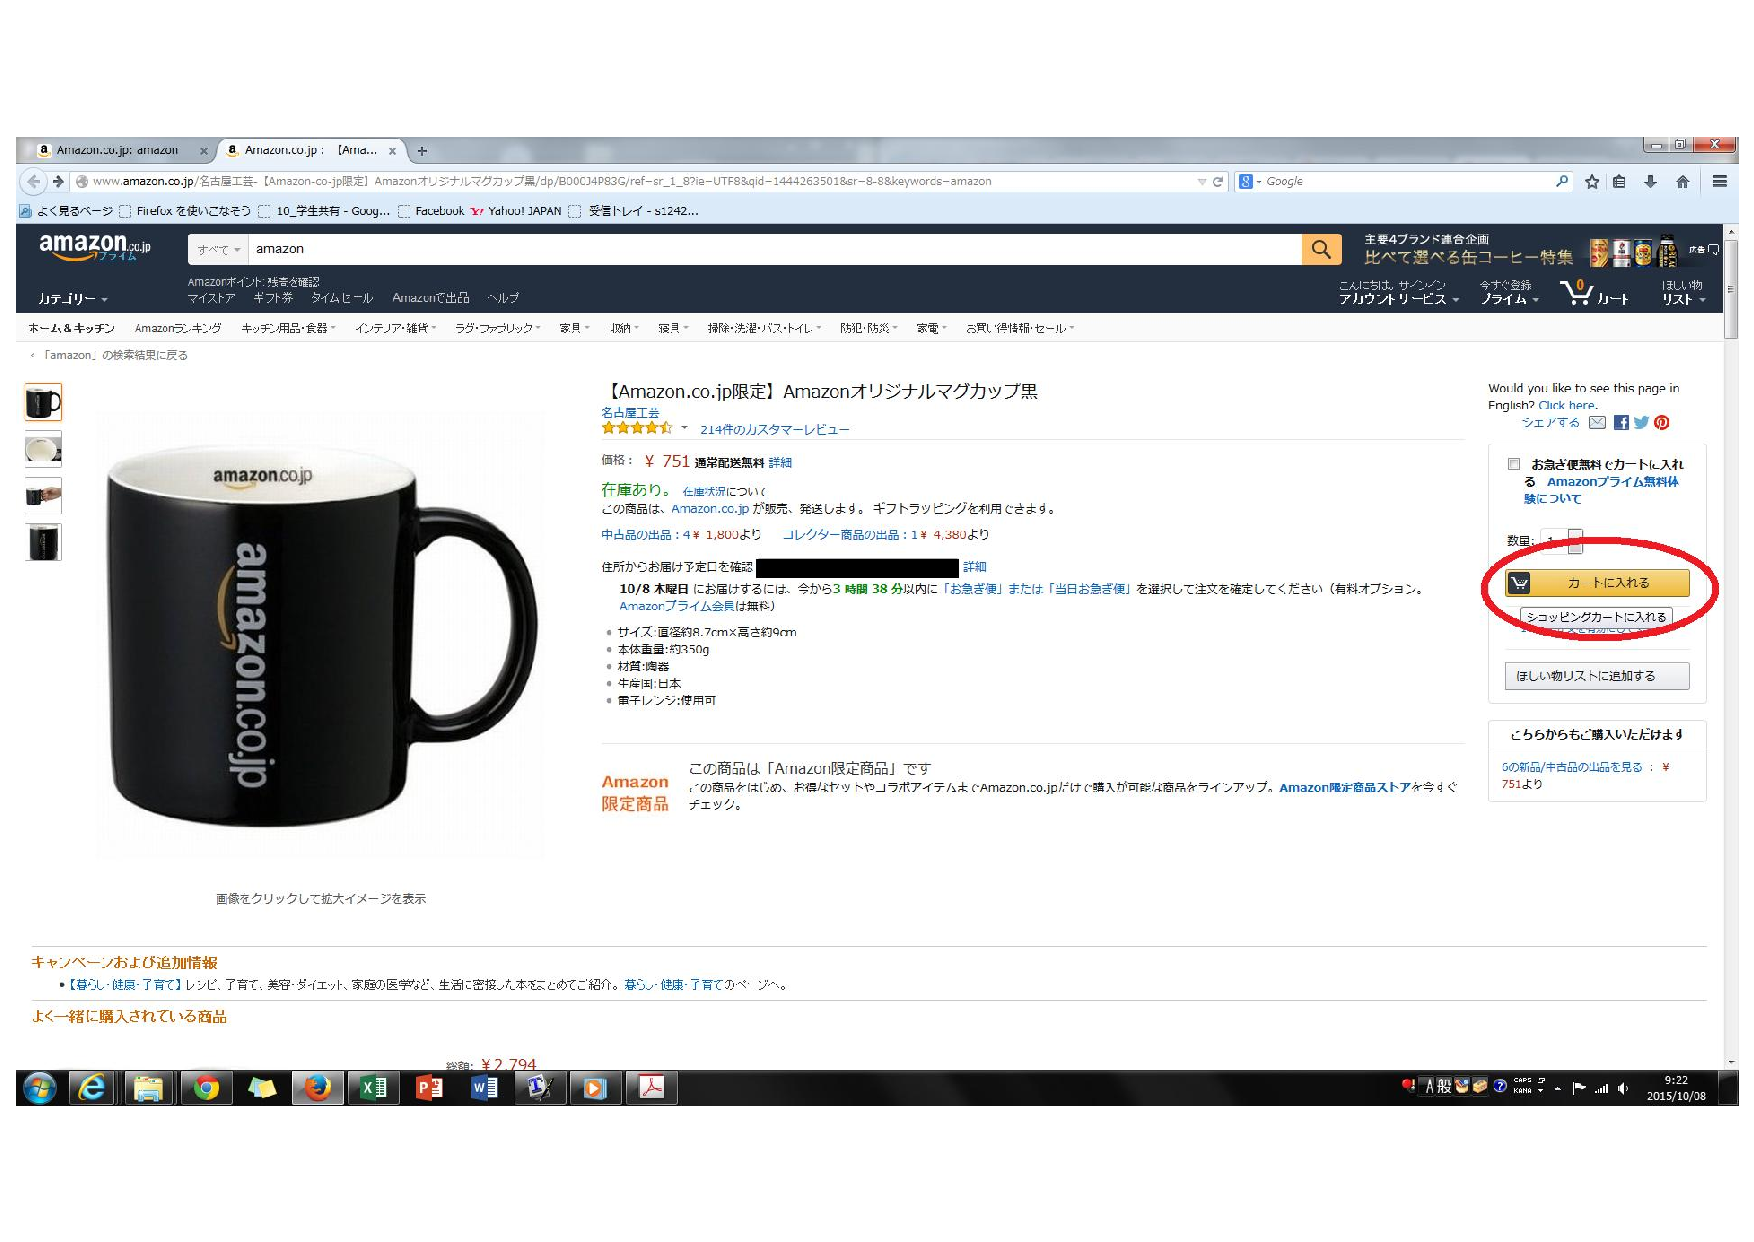
\includegraphics[width=10cm]{kensakuhouhou2.pdf}
\caption{Amazonでの購入解説2}
\label{Amazonでの購入解説2}
\end{figure}




 \item 画面が移動した場合次のような項目が表示(\ref{Amazonでの購入解説3})されるので,赤丸の印の部分の「レジへ進む」をクリックすることで次の画面に移動する.

%図の挿入
\begin{figure}[htb]
\centering
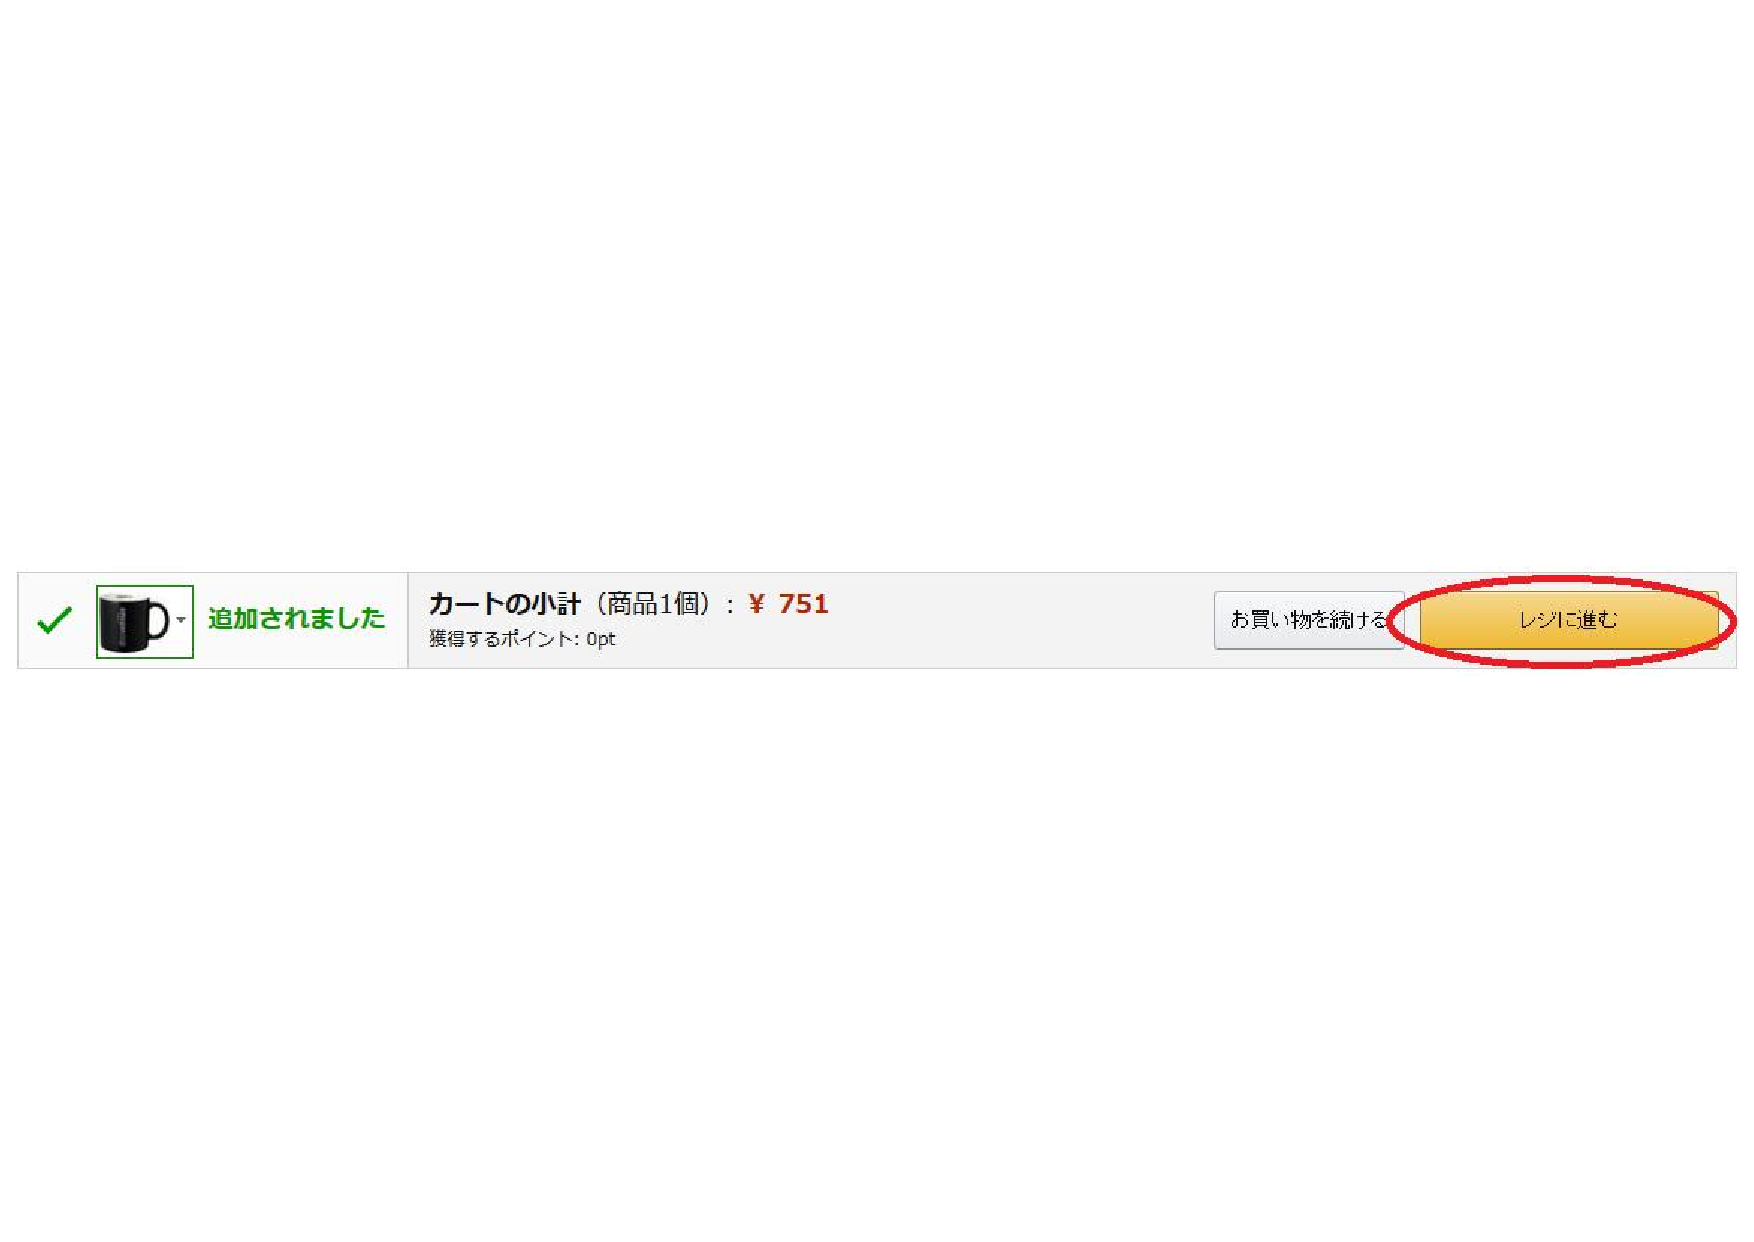
\includegraphics[width=10cm]{kensakuhouhou3.pdf}
\caption{Amazonでの購入解説3}
\label{Amazonでの購入解説3}
\end{figure}


\clearpage

 \item 画面が移動した場合次のような画面が表示(\ref{Amazonでの購入解説4})されるので,赤丸の印の部分の「初めて利用します。」をクリックし選択後,「サインイン」をクリックしてアカウントの新規作成を行う.


%図の挿入
\begin{figure}[htb]
\centering
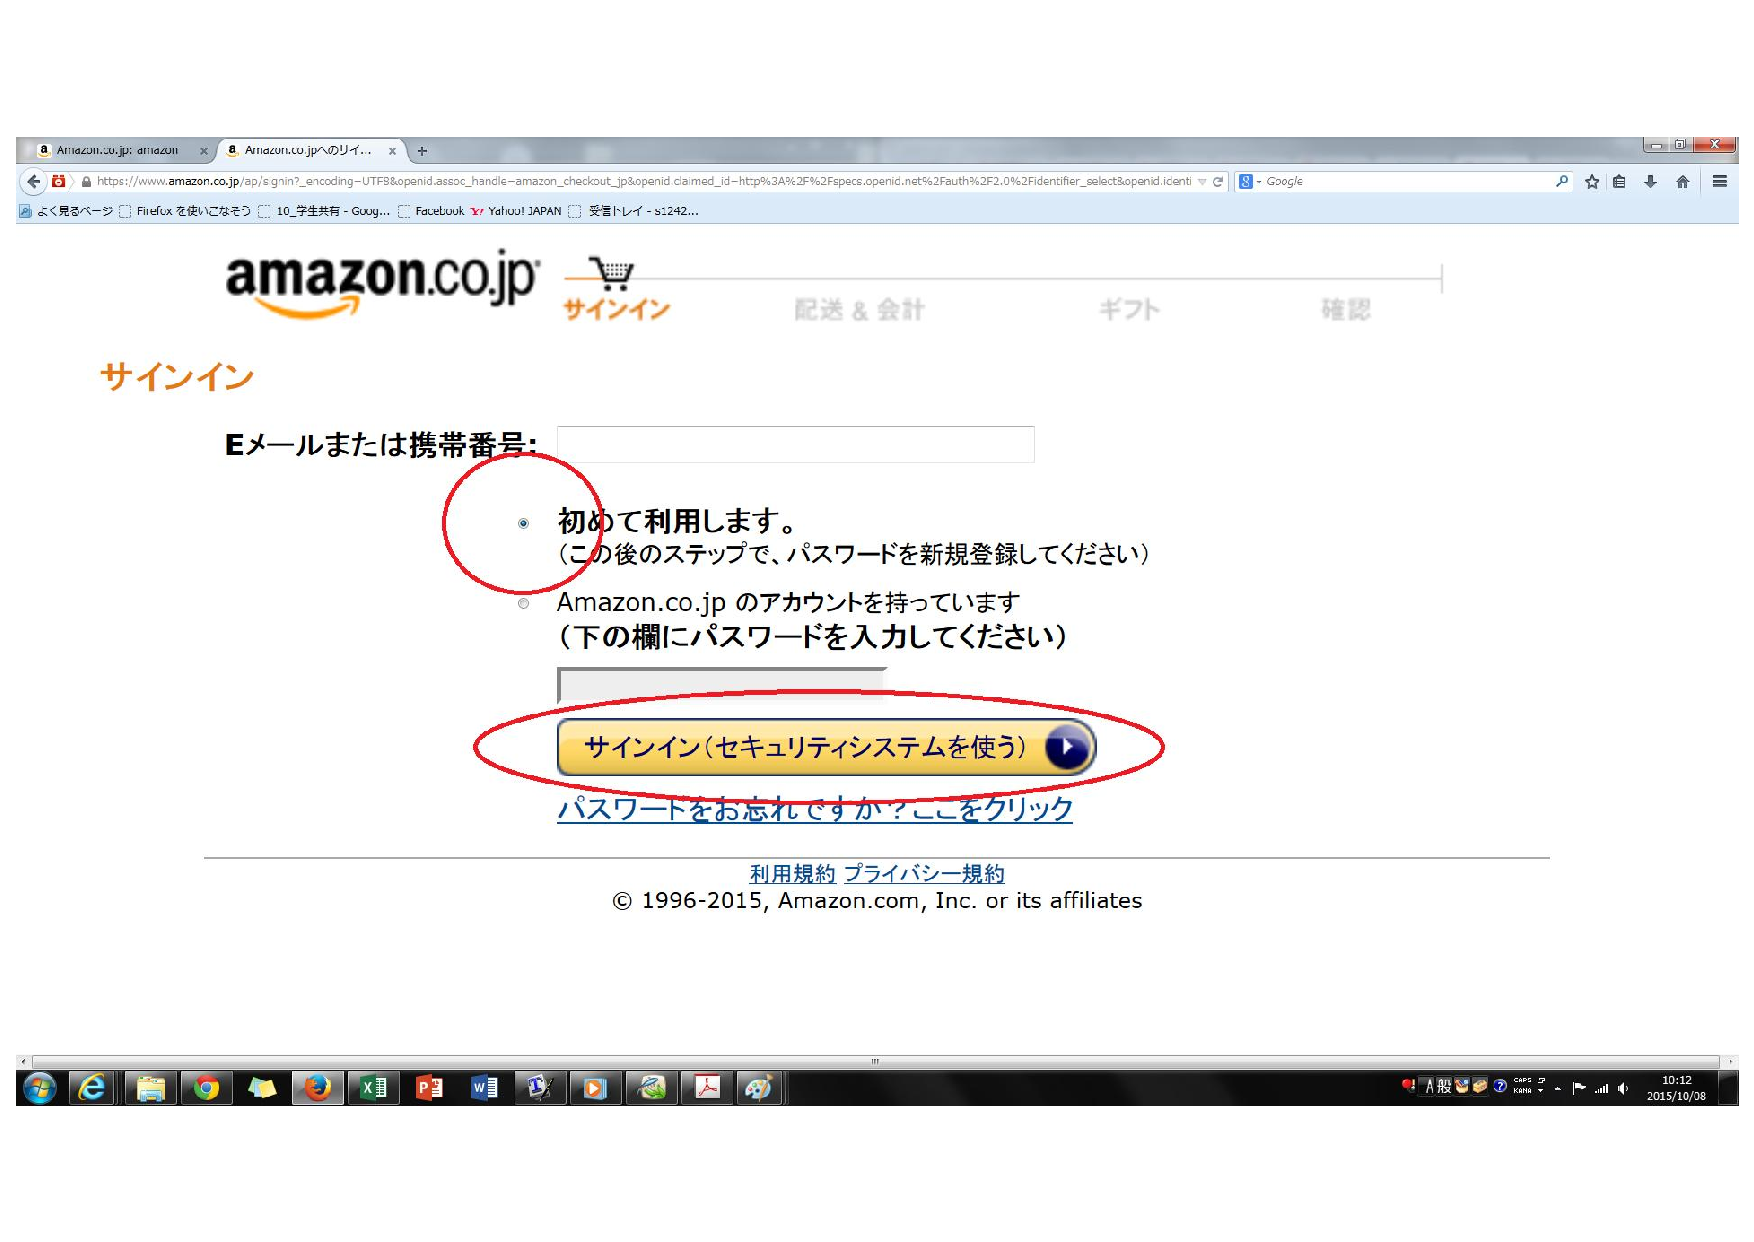
\includegraphics[width=10cm]{kensakuhouhou4.pdf}
\caption{Amazonでの購入解説4}
\label{Amazonでの購入解説4}
\end{figure}






\item アカウントの作成後この画面が表示(\ref{Amazonでの購入解説5})されていれば注文は確定され成功である.

%図の挿入
\begin{figure}[htb]
\centering
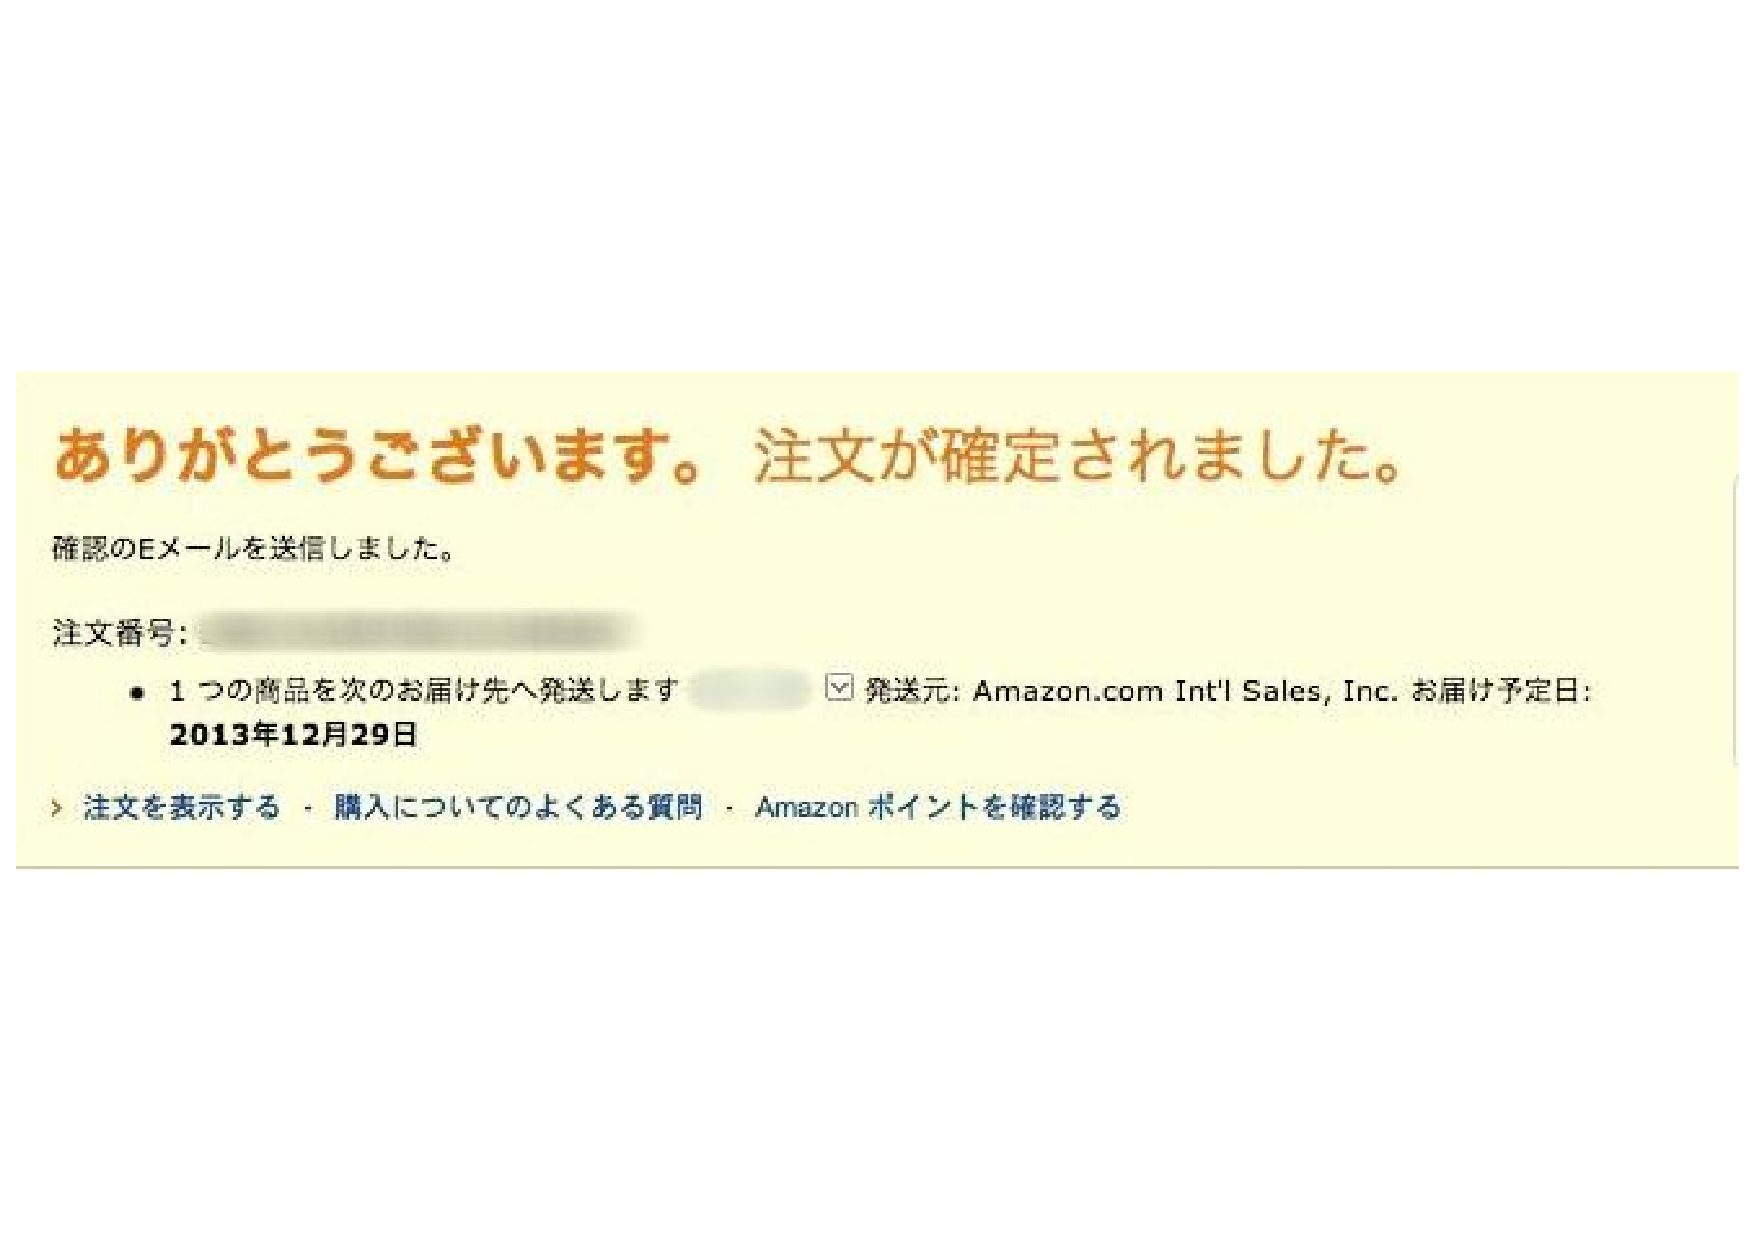
\includegraphics[width=10cm]{kensakuhouhou5.pdf}
\caption{Amazonでの購入解説5}
\label{Amazonでの購入解説5}
\end{figure}


\end{enumerate}




\clearpage




\subsubsection{商品の購入方法から繋がるレビューの問題点}

Amazonではクレジットカード,代金引換,コンビニ支払いの三種の支払い方法から選択して決済を行う.
決済の完了が確認され次第,商品の配送が行われ翌日から一週間ほどの期間を経て指定場所へ届く.
この決済方法での問題から商品到着までの過程で問題が発生した場合商品レビューにも影響を及ぼすケースが存在する.
店舗ごとに存在する特典配布の差異,などがあげられる.
それらの例として


\begin{itemize}


 \item	特典の問題


\begin{itemize}
\setlength{\parskip}{3mm}


 \item	例:実際に投稿されたレビューの抜き出し

「まだ間に合います


49人中、17人の方が、「このレビューが参考になった」と投票しています。
5つ星のうち1.0

投稿者○○○○ 2012年9月2日

9/1ヤ○ダ電気で確認したところ早期購入特典が付いてくるとのことでしたので、買い直しました。Amazon分は返品します。
家電量販店など大量に仕入れているところでは特典が余っている可能性大です。特典が諦めきれない方はお近くの量販店に行ってみては如何ですか?

Amazonの中の人は、何ヶ月も前から予約している人が何を目的としているのか少し考えてみてください。
次回から特典物がほしい場合はAmazonは利用しません。
評価はAmazonで買った場合の評価です。ゲーム内容は★5ですが、ここで買うのはおすすめできません」


 \item	商品の公式ページにて記載された情報

全国のゲーム取り扱い店及び下記店舗にて予約受付中です。
先着購入特典の有無は各店舗様にお問い合わせ下さい。

ちなみに公式のこのページに書いてあるのは取り扱い店のリンクであり、“特典の付く店のリンク”ではありません
先着購入特典や店舗別予約特典のページは下記のページです



\end{itemize}


\end{itemize}

このようにレビューを記載した人物が商品への理解が足りずそれを原因として評価を下げているケースが見受けられる.

これらのレビューに対する評価として「レビューを見た人」の中の「参考になったと回答した人」の割合は低いことが分かる.
よって商品のレビューの平均点をそのまま記載するという方法に比べて,これら割合を考慮した場合のほうがより正確になるという予測が立てられる.




\clearpage



\section{Amazonでの商品のレビューの手順}

本項目ではオンラインショッピングにおける業界最大手であるAmazonでの商品のレビューの手順を解説していく.

\subsubsection{商品のレビューの方法}

\begin{enumerate}

\item 評価したい商品の画面(\ref{Amazonでのレビューの解説})に移動し,矢印の方向(下)にスクロールする.

%図の挿入
\begin{figure}[htb]
\centering
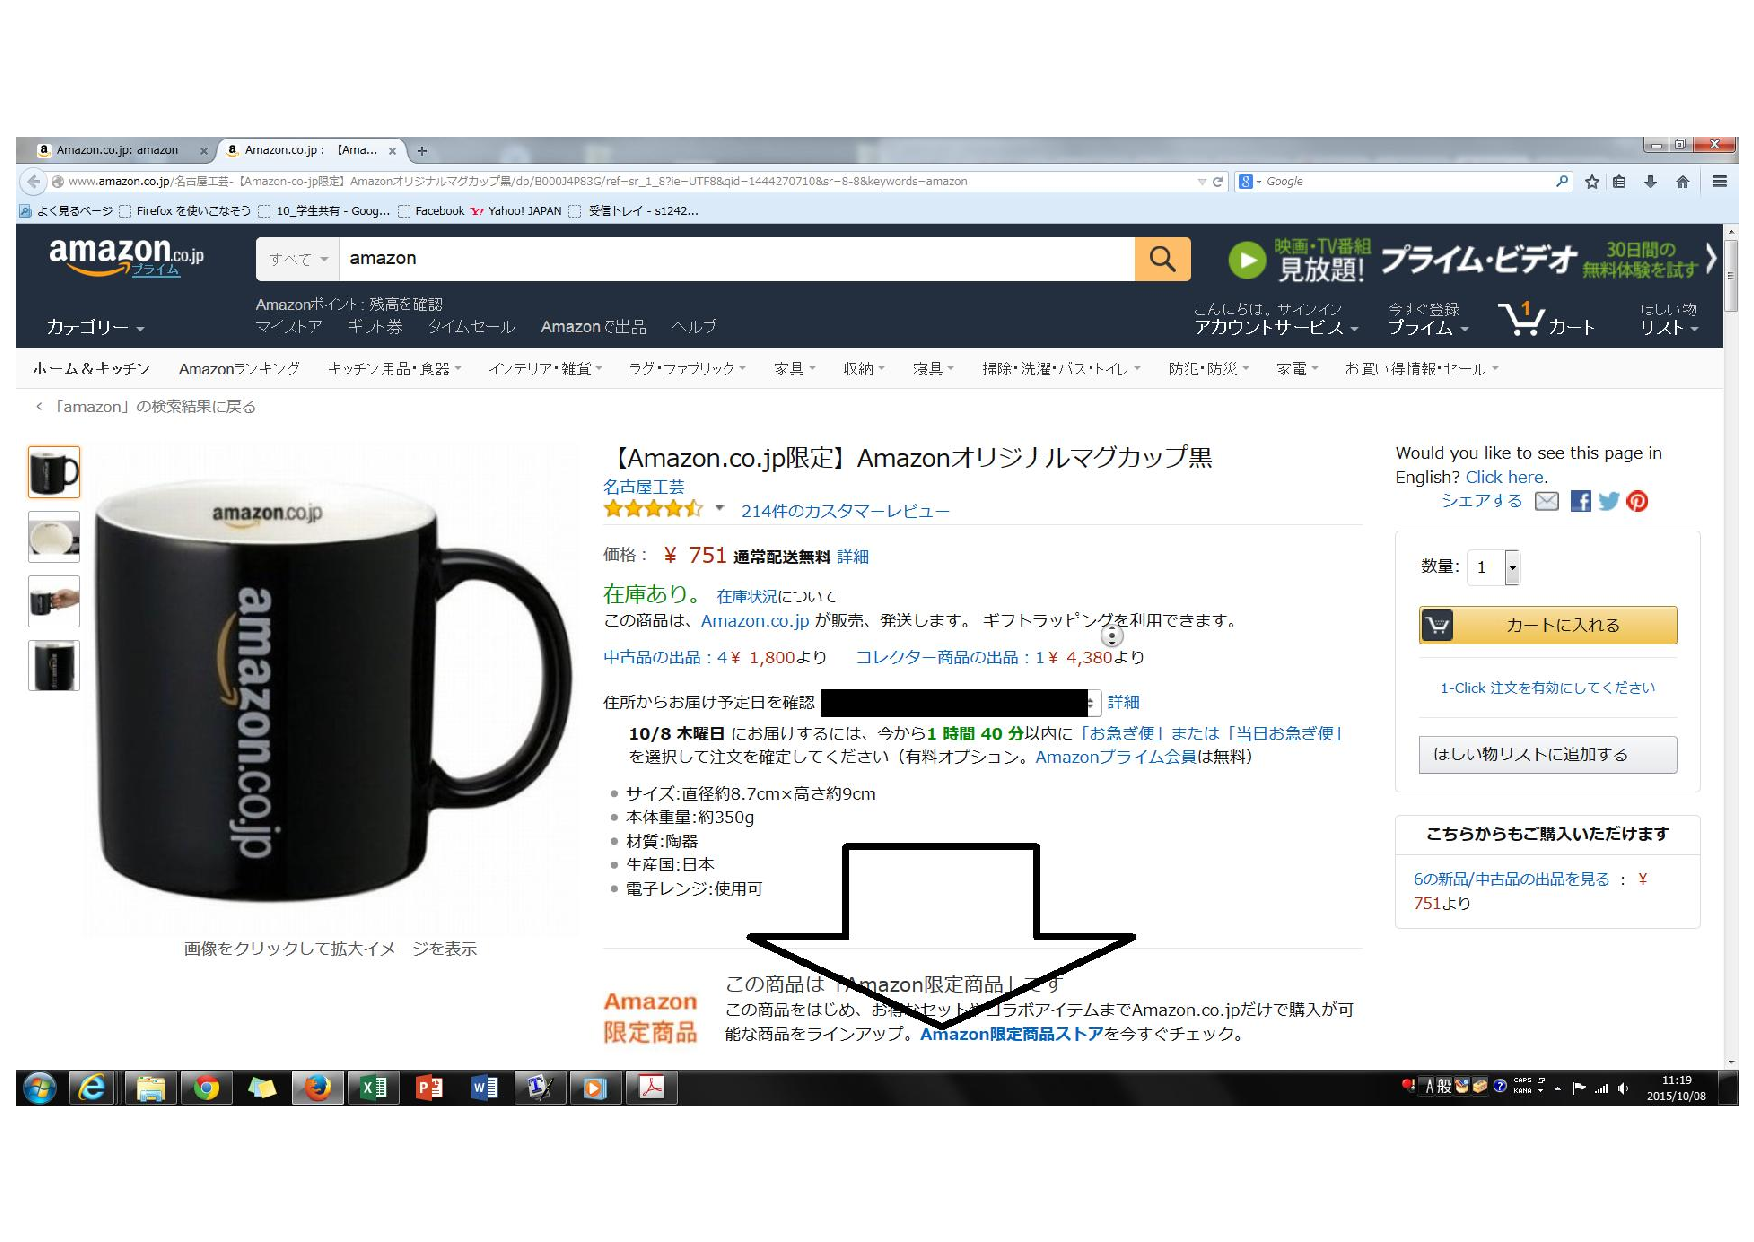
\includegraphics[width=10cm]{reviewhouhou.pdf}
\caption{Amazonでのレビューの解説}
\label{Amazonでのレビューの解説}
\end{figure}

 \item スクロールすると「カスタマーレビュー」の画面が表示(\ref{Amazonでのレビューの解説2})される.その赤丸の印の部分の「カスタマーレビューを書く」をクリックする.

%図の挿入
\begin{figure}[htb]
\centering
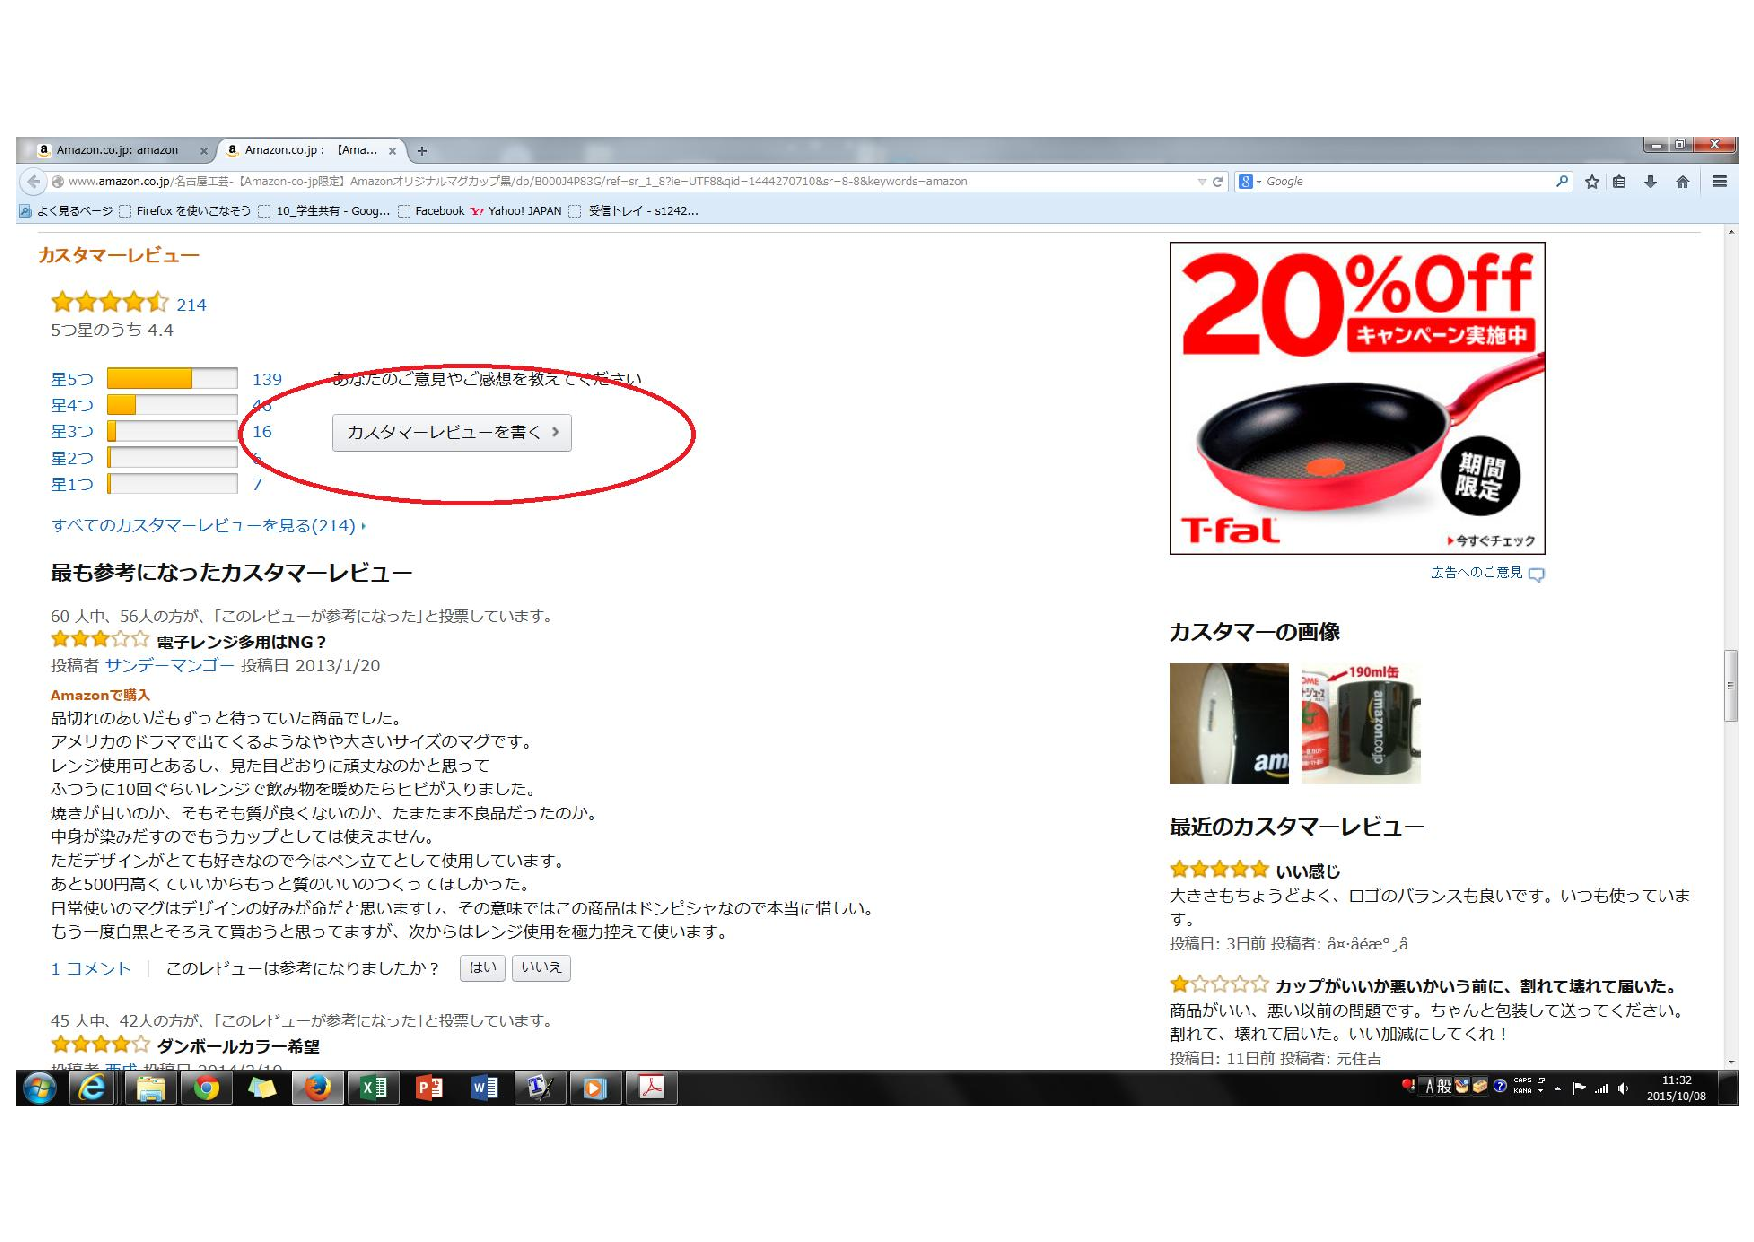
\includegraphics[width=9cm]{reviewhouhou2.pdf}
\caption{Amazonでのレビューの解説2}
\label{Amazonでのレビューの解説2}
\end{figure}








\clearpage







%図の挿入
\begin{figure}[htb]
\centering
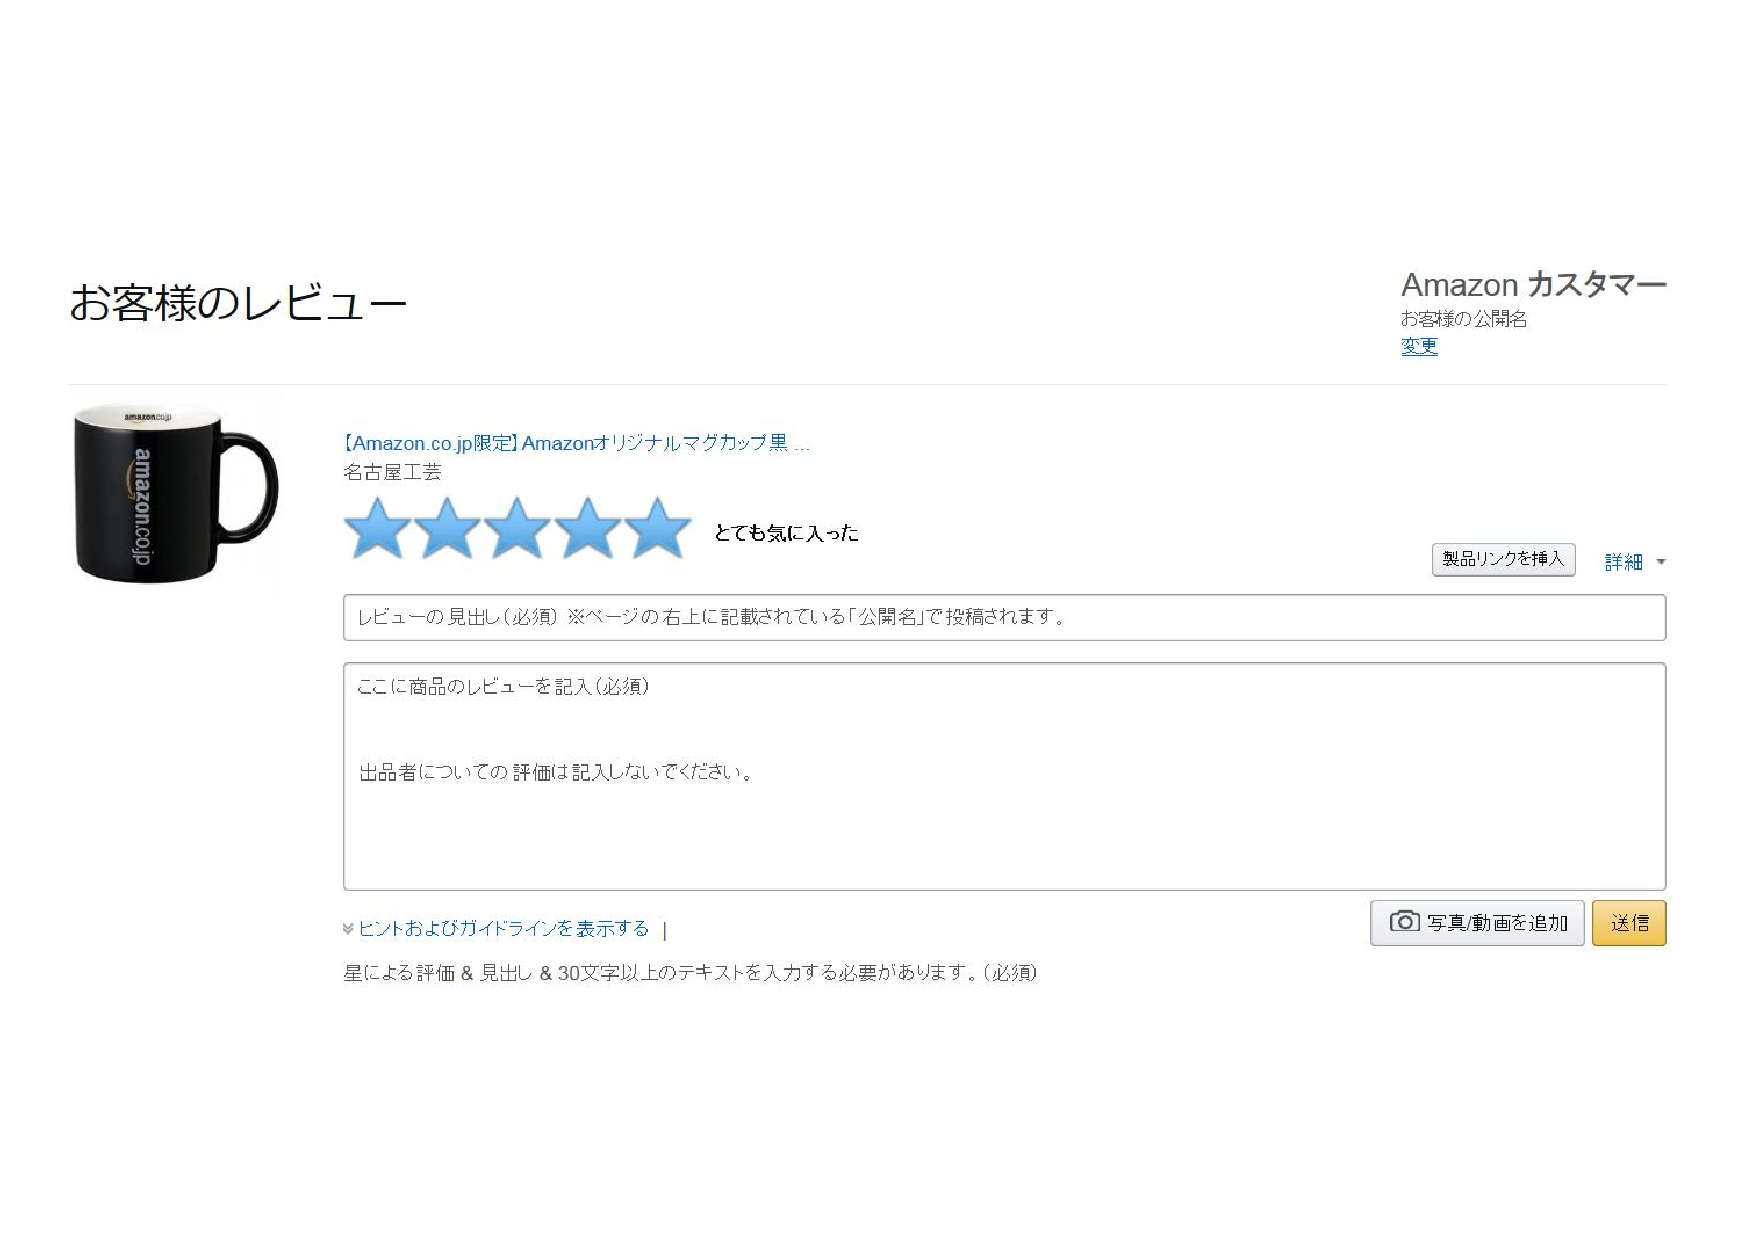
\includegraphics[width=8cm]{reviewhouhou3.pdf}
\caption{Amazonでのレビューの解説3}
\label{Amazonでのレビューの解説3}
\end{figure}

 \item 「カスタマーレビューを書く」をクリックするとこのような画面(\ref{Amazonでのレビューの解説3})が表示される.☆のマークに評価したい段階でマウスカーソルを合わせ,クリックすることで5段階評価が行える.
 \item 枠内の項目に題名,コメントを記入する.
 \item 記入が終わり次第,「送信」ボタンをクリックすることでレビューの登校が完了する.


\end{enumerate}


\chapter{クローラーについて}


本研究はオンラインショッピングのレビューを調査を行う必要がある.
しかし,各サイトのレビューページのレビューは数ページにわたり,個人が手動で分析するには限界がある.
クローラーを利用することで飛躍的に作業効率が上がる.

よって本研究ではクローラーを使用し,レビューデータを統計している.

\section{クローラーとは}

クローラーとは,システムが自動的にWebページを巡回して情報を収集するプログラムである.クローラーとして最も有名なのは,Googleなどの検索エンジンがあげられる.

クローラーはビジネスの場面でも使われている.マーケティング分析では,掲示板やSNSの書き込みをクローラーで見て回ることが可能だ.SNSに自動ログインして情報収集するクローラーも存在する.

個人用途であってもクローラーが使われる.特定のページを定期的にアクセスして更新を自動チェックしたり,ページの内容を整形して表示するプログラムも広い意味でクローラーになりうる.それらを駆使すれば情報収集の時間が短縮できる\cite{sasakitakurou2014}.


主に検索エンジンのデータベース,インデックス作成に用いられているほか,統計調査などの目的にも利用される.

一般にクローラ,既知のHTML文書の新しいコピーを要求し,文書中に含まれるリンクをたどり別の文書を収集するという動作を繰り返す.新しい文書を見つけた場合はデータベースに登録する.


\section{主なクローラー}


\begin{itemize}
\setlength{\parskip}{3mm}

 \item	グーグルボット(Googlebot、Google)

 \item	bingbot(英語版)(マイクロソフト・bing)

 \item	Baiduspider(百度)

 \item	Yetibot(ネイバー)

\end{itemize}



\chapter{Ubuntuについて}

本研究では統計を収集するに当たりUbuntuを使用することとした.



\section{Ubuntuとは}

Ubuntuは,Linuxをベースとしたオペレーティングシステムである.オープンウェアとして提供されている.
Ubuntuの開発目標は、「誰にでも使いやすい最新かつ安定したOS」を提供することである.Ubuntuという名称は、南アフリカのズールー語の言葉で「他者への思いやり」を意味する 
Ubuntuはカノニカル社から支援を受けて開発されている.\cite{Ubuntu2015}


\begin{itemize}

 \item	特徴

\begin{itemize}
\setlength{\parskip}{3mm}


 \item	Linuxというボランティアの集まりによってフリーかつ,オープンなオペレーティングシステムをベースとして作られている.

 \item	Ubuntuは、アフリカの単語で「他者への思いやり」や「皆があっての私」といった意味を含めて名付けられた.

 \item	Ubuntuは,コミュニティにより開発されているオペレーティングシステムである.

 \item	2015時点で,無償で提供し,将来に渡り無料を継続し続ける予定である.

 \item	新しいデスクトップ及びサーバーを6ヶ月ごとにリリースすることを宣言している.


\end{itemize}

 \item	歴史

\begin{itemize}
\setlength{\parskip}{3mm}

 \item	Ubuntu の最初のリリースは,2004年10月20日にDebian GNU/Linuxから派生したものである.
2005年7月8日,マーク・シャトルワースとカノニカルはUbuntu財団を創設し,初期投資として1000万USドルを提供したと発表した.
財団の目的は,今後リリースされるバージョンも含めたUbuntuのサポートと開発を保証することであるが,2006年時点で財団は休眠状態にある.この不透明な状況をマーク・シャトルワースは,財団はCanonicalに不測の事態が起きたときの緊急財源であると説明している.

2008年9月5日、DELLが発表したミニノートPC「Inspiron Mini 9」は、OSにUbuntuを選択可能だ.さらに,2009年8月27日にシャープが発表したスマートブック「NetWalker」には,Ubuntu 9.04がプリインストールされている.\cite{Ubuntu}

\end{itemize}
\end{itemize}



\section{派生品について}


Ubuntuと異なるパッケージではあるが,Ubuntuと同じリポジトリで管理されているので,お互いに全く同じパッケージが使用可能であり,それぞれのデスクトップ環境を共存させられる。

\begin{itemize}
\setlength{\parskip}{3mm}

 \item	Edubuntu

教育用にカスタマイズされたもの.児童が学校や自宅で同等の環境を利用できることを目的としている.

 \item	Gobuntu

フリーソフトウェアのみを利用したディストリビューションである.

 \item	Kubuntu

Ubuntuのデスクトップ環境を KDE に置き換えたものである.

 \item	Lubuntu

Ubuntuのデスクトップ環境を LXDE に置き換えたものである.

 \item	Mythbuntu

UbuntuとMythTVを元に作られた,ホームシアターPC向けのディストリビューションである.

 \item	Ubuntu for Android

Android端末向けのディストリビューションである.

 \item	Ubuntu GNOME

Ubuntuのデスクトップシェルを GNOME Shell に置き換えたものである.

 \item	Ubuntu Desktop 日本語 Remix

Ubuntu Japanese Teamによって日本語化されたものである.

 \item	Ubuntu Kylin

中国向けに開発されたディストリビューションである.

 \item	Ubuntu MATE

MATEと呼ばれるデスクトップ環境を採用したものである.

 \item	Ubuntu Netbook Edition

ネットブック等の小型端末向けのディストリビューション.

 \item	Ubuntu Server

サーバー向けのディストリビューションである.

 \item	Ubuntu Studio

クリエイター向けのディストリビューションである.

 \item	Ubuntu Touch

組み込み端末向けに作成されたディスリビューションであり,Ubuntu Mobileの後継版である.

 \item	Ubuntu TV

スマートTV向けのディストリビューションである.

 %\item	Xubuntu

%Ubuntu のデスクトップ環境を Xfce に置き換えたものである.

\end{itemize}


\clearpage


\section{リリース期間とサポート期間}



\begin{table}[htb]
\label{Ubuntuリリース時期とサポート期間}
\caption{Ubuntuリリース時期とサポート期間}
\newlength{\Ubuntusupport}
\setlength{\Ubuntusupport}{0.6cm}
  \begin{center}

	\begin{tabular}{|r|r|r|r|}

 \hline

	コードネーム & バージョン & リリース日 & サポート期限 \\ \hline \hline

	\parbox[c][\Ubuntusupport][c]{0cm}{}
	Xenial Xerus & 16.04 LTS & 2016年4月21日(予定) & 2021年4月 \\

	\parbox[c][\Ubuntusupport][c]{0cm}{}
	Wily Werewolf & 15.10 & 2015年10月22日 & 2016年7月 \\

	\parbox[c][\Ubuntusupport][c]{0cm}{}
	Vivid Vervet & 15.04 & 2015年4月23日 & 	2016年1月 \\

	\parbox[c][\Ubuntusupport][c]{0cm}{}
	Trusty Tahr & 14.04 LTS & 2014年4月17日 & 2019年4月 \\

	\parbox[c][\Ubuntusupport][c]{0cm}{}
	Precise Pangolin & 12.04 LTS & 2012年4月26日 & 2017年4月 \\

	\parbox[c][\Ubuntusupport][c]{0cm}{}
	Utopic Unicorn & 14.10 & 2014年10月23日 & 2015年7月 \\

	\parbox[c][\Ubuntusupport][c]{0cm}{}
	Saucy Salamander & 13.10 & 2013年10月17日 & 2014年7月 \\

	\parbox[c][\Ubuntusupport][c]{0cm}{}
	Raring Ringtail & 13.04 & 2013年4月25日 & 2014年1月 \\

	\parbox[c][\Ubuntusupport][c]{0cm}{}
	Quantal Quetzal & 12.10 & 2012年10月18日 & 2014年4月 \\

	\parbox[c][\Ubuntusupport][c]{0cm}{}
	Oneiric Ocelot & 11.10 & 2011年10月13日 & 2013年5月 \\

	\parbox[c][\Ubuntusupport][c]{0cm}{}
	Natty Narwhal & 11.04 & 2011年4月28日 & 2012年10月 \\

	\parbox[c][\Ubuntusupport][c]{0cm}{}
	Lucid Lynx & 10.04 LTS & 2010年4月29日 & 2013年5月9日 \\

	\parbox[c][\Ubuntusupport][c]{0cm}{}
	Karmic Koala & 9.10 & 2009年10月29日 & 2011年4月 \\

	\parbox[c][\Ubuntusupport][c]{0cm}{}
	Jaunty Jackalope & 9.04 & 2009年4月23日 & 2010年10月 \\

	\parbox[c][\Ubuntusupport][c]{0cm}{}
	Hardy Heron & 8.04 LTS & 2008年4月24日 & 2011年4月 \\

	\parbox[c][\Ubuntusupport][c]{0cm}{}
	Gutsy Gibbon & 7.10 & 2007年10月18日 & 2009年4月 \\

	\parbox[c][\Ubuntusupport][c]{0cm}{}
	Edgy Eft & 	6.10 & 2006年10月26日 & 2008年4月 \\

	\parbox[c][\Ubuntusupport][c]{0cm}{}
	Dapper Drake & 6.06 LTS & 2006年6月1日 & 2009年7月14日 \\

	\parbox[c][\Ubuntusupport][c]{0cm}{}
	Breezy Badger & 5.10 & 2005年10月13日 & 2007年4月 \\

	\parbox[c][\Ubuntusupport][c]{0cm}{}
	Hoary Hedgehog & 5.04 & 2005年4月8日 & 2006年10月 \\

	\parbox[c][\Ubuntusupport][c]{0cm}{}
	Warty Warthog & 4.10 & 2004年10月20日 & 	2006年4月 \\

	\hline

	\end{tabular}
\end{center}
\end{table}

\chapter{VirtualBoxについて}

Ubuntuを使用するにあたり,自身の環境がwindowsであったため仮想環境での構築が必要であった.

そこでVirtualBoxを使用することで,Ubuntuの仮想環境を作成した.

\section{VirtuualBoxとは}

既存のオペレーティング・システム上にアプリケーションとしてインストールすることで,コンピュータ上に追加のオペレーティング・システムを実行することができる。


\begin{itemize}

 \item	例

\begin{itemize}
\setlength{\parskip}{3mm}


 \item	WindowsXPがオペレーション・システム として動作しているマシン上で、Linuxをゲストとすることができる

 \item	Solarisが実行されているコンピュータ上で,Windows Vistaをゲストとして実行する

\end{itemize}


 \item	特徴

\begin{itemize}
\setlength{\parskip}{3mm}

 \item	無償のオープンソース仮想化ソフトウェア

 \item	多くの32bit/64bitOS上で動作可能

 \item	ホスト型のHypervisor

 \item	ゲストOSをRDPで操作可能

 \item	幅広いUSBデバイスをサポート

 \item	ACPIをフルサポート

 \item	スナップショットに対応し、ゲストOSの状態を複数保存可能

 \item	NICはNATやブリッジ、内部ネットワークなどをサポート

 \item	iSCSIをサポート

 \item	PXEブートをサポート

 \item	マルチスクリーンに対応

 \item	共有フォルダを使い、ホストOSとゲストOS間でファイルの共有が可能

 \item	1つのディスクを複数の仮想マシンで共有する共有ディスク機能

 \item	CPUのホットプラグ機能

 \item	ゲストOS間でメモリをやり取りするメモリバルーニング機能

\end{itemize}


 \item	歴史

\begin{itemize}
\setlength{\parskip}{3mm}

 \item	当初はプロプライエタリ・ソフトウェア・ライセンスで提供され,製品VirtualBoxのある版は,個人的あるいは評価の使用に対してのみ無料であり,「VirtualBox Personal Use and Evaluation Licence (PUEL)」が適用された.2007年1月数年の開発の後,VirtualBox OSE(Open Source Edition)がフリーソフトウェアとして,商用と個人的な使用のためにリリースされ,GNU General Public License (GPL),version2が適用された.

\end{itemize}

 \item	機能

\begin{itemize}
\setlength{\parskip}{3mm}


 \item	スナップショット

 \item	シームレス・モード

 \item	クリップボード

 \item	共有フォルダ

 \item	シリアルデバイスと,システム間の切替えを支援するユーティリティ

 \item	コマンドラインからの操作

 \item	リモート・ディスプレイ

 \item	64ビット・ゲスト

 \item	AMD-V と VT-xのための,入れ子

 \item	3Dアクセラレーション


\end{itemize}

\end{itemize}



\chapter{目的}



日本の大手サイトであるAmazon,楽天,Yahoo!ショッピングなどはレビューを5段階で表記し,その内訳は平均値である.
他にも詳細を記載している部分もあるが,どのサイトも総合評価として大きく記載している部分は平均値で共通する.

例として画像に乗せる(図\ref{customerReview})(図\ref{rakutenReview})(図\ref{Yahoo!Review}).

図\ref{rakutenReview}

\begin{figure}[htbp]

\centering
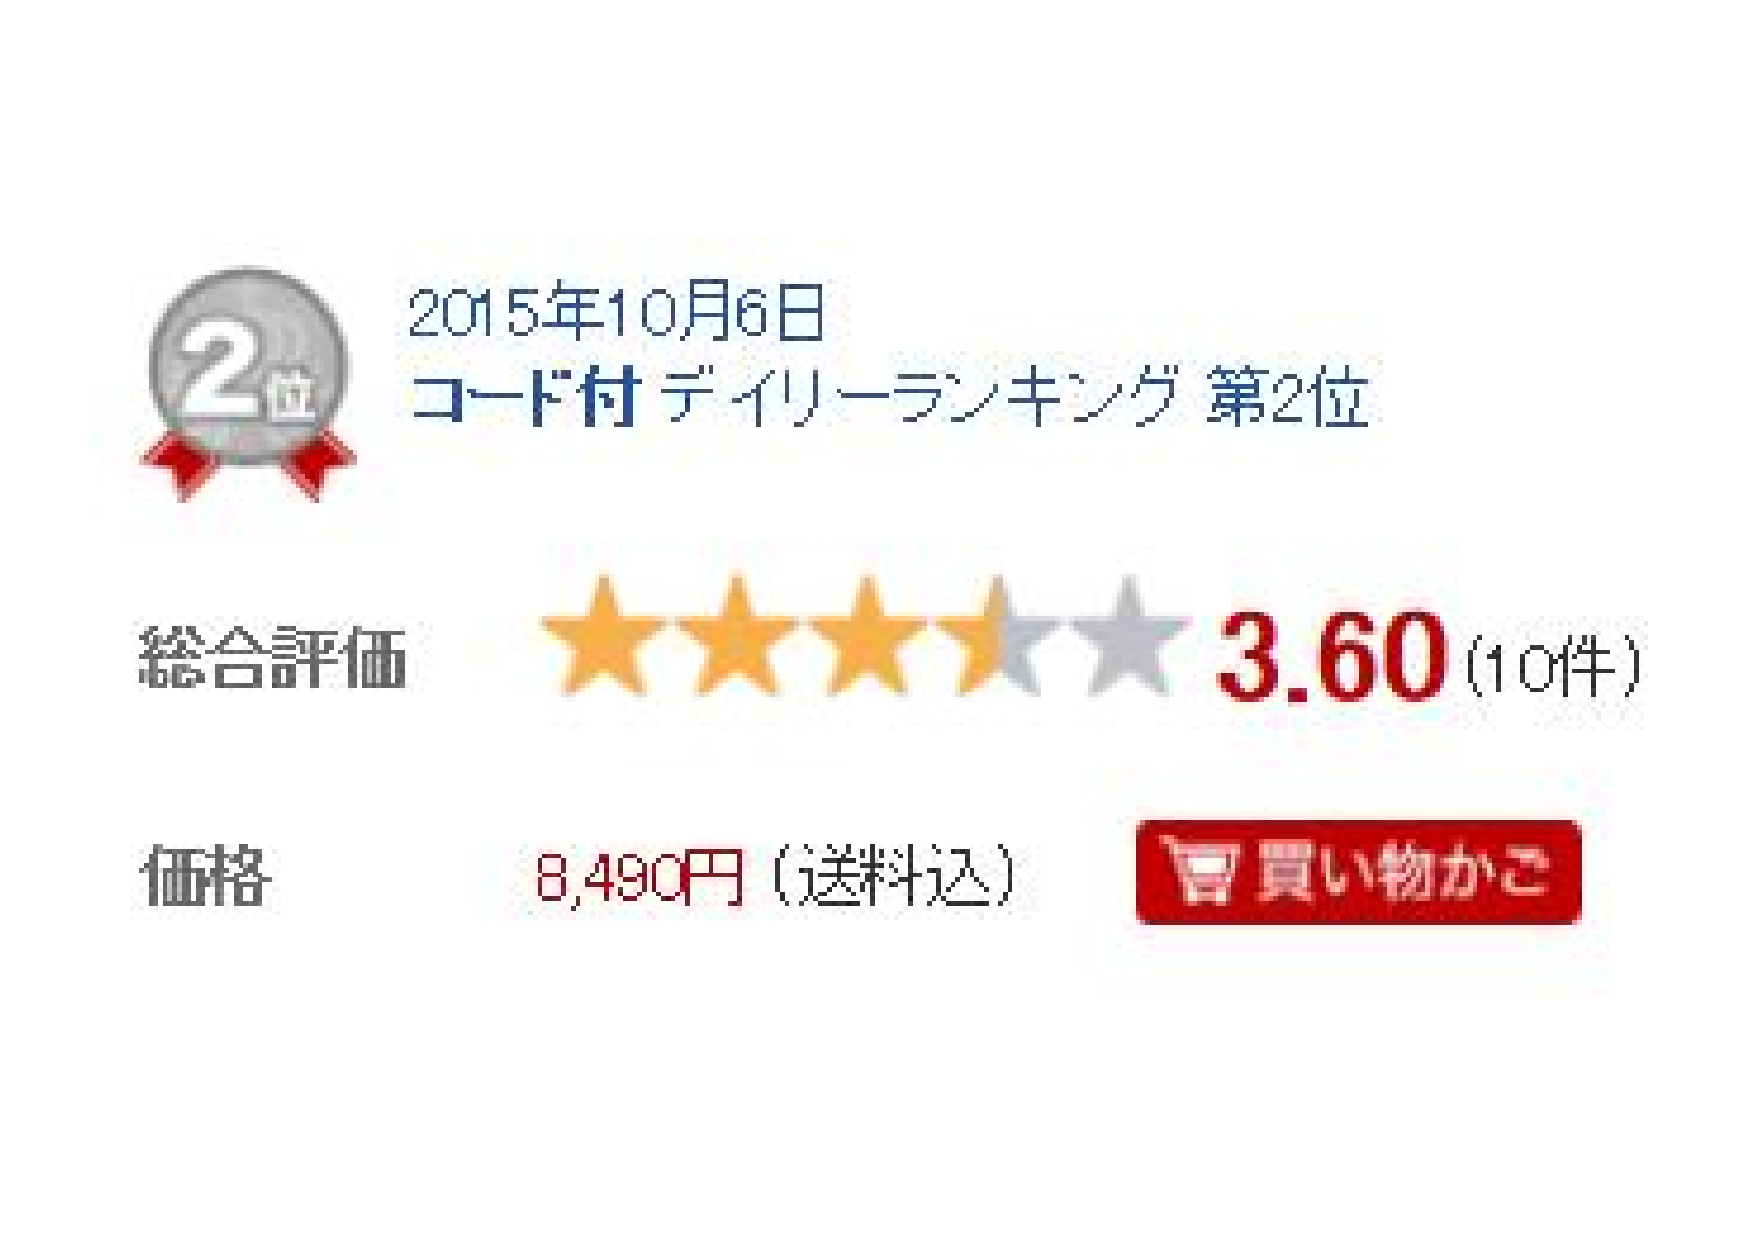
\includegraphics[width=7cm,clip]{rakutenReview.pdf}
\caption{楽天でのレビューの一例}
\label{rakutenReview}

\end{figure}

図\ref{Yahoo!Review}

\begin{figure}[htbp]

\centering
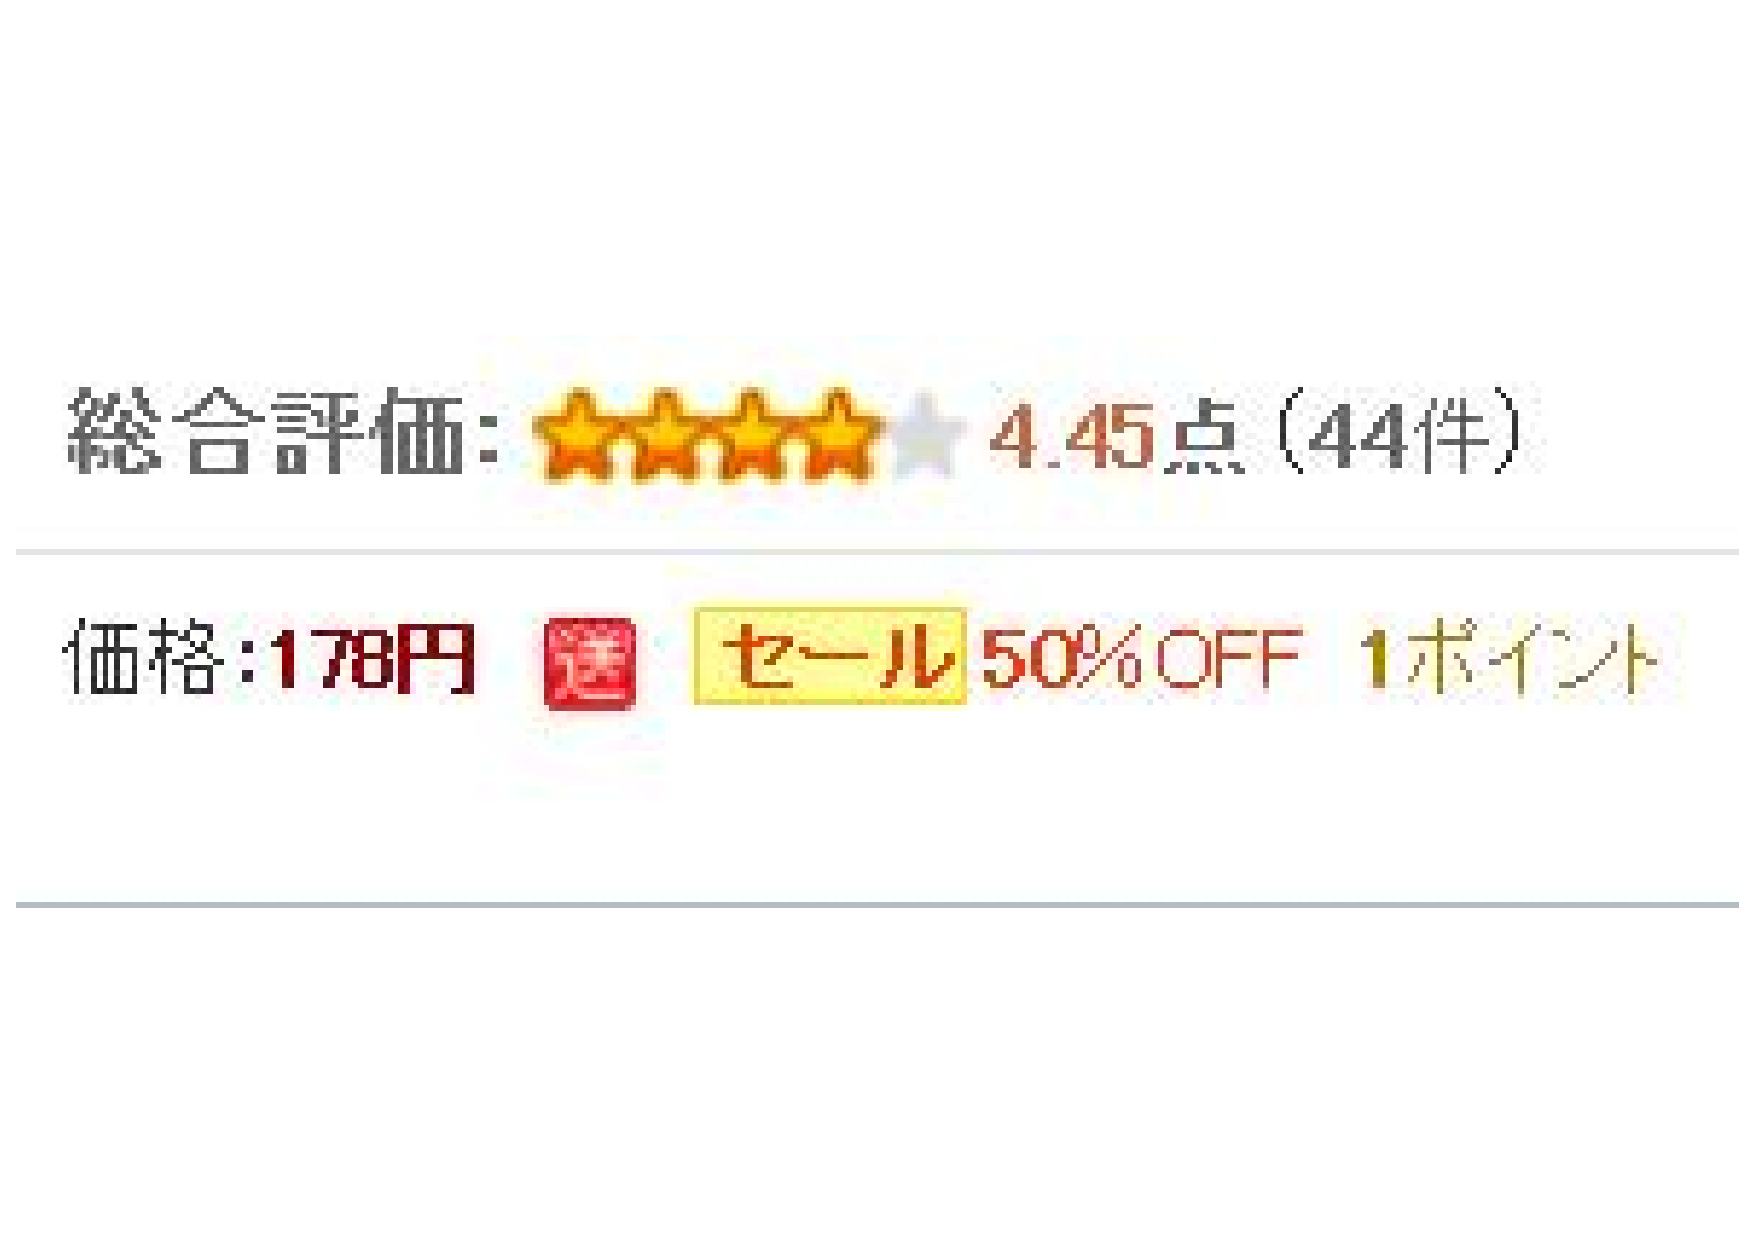
\includegraphics[width=7cm,clip]{Yahoo!Review.pdf}
\caption{Yahoo!ショッピングでのレビューの一例}
\label{Yahoo!Review}

\end{figure}




平均値のみでは総合評価の信頼性が記入者に依存する形となる.
よってそのレビューが不適切な内容で商品の参考にならなければレビューとして意味をなさないにも関わらず加算してしまう.

\begin{itemize}

 \item	総合評価として付け足すべきではない例

\begin{itemize}
\setlength{\parskip}{3mm}
 \item	商品の評価が嘘偽りの場合,実際になかった内容であるためのレビュー.
 \item	無関係の場合,幾ら高い評価,低い評価であったとしても商品そのものを評価していない.

これらのレビューは平均評価で出す場合はそれらのレビューを入れた状態のまま反映してしまう.そのためレビューの信頼が低いと判断した.


\end{itemize}

\end{itemize}


どのレビューが信頼が低いかを判断するためにも,どの程度信用できるかを判断できる重みをレビューに付け足すことで信頼度をあげていく.

そこで重みを付けるために記入者に対する絞込みを行う,もしくは回覧者を利用することで個々のレビューに対してどの程度信頼できるかなどの絞込みを行う.
これらやこれらに準ずる絞込みを行うことで指標を作り出していく.

このような他の指標を加え判断材料を増やすことで,平均値のみの表示よりも信頼できるレビューを作ることが目的である.


\chapter{プロジェクトマネジメントとの関連性}


PMBOKにおける10個の知識体系エリアのひとつとして品質マネジメントがある.その内容には

「品質コントロールの最終的な目標は,成果物の正しさを決定することである.」\cite{pmbok2013}

と記述されている.

レビュー評価の信頼性が向上することでオンラインショッピングサイトのレビューを利用したプロジェクトも信頼性が高まると言える.
よってその成果物の正しさを証明しやすくなる.




\chapter{手法}

\section{データ対象の決定と処理言語の決定}
アクセス数,資本金を比較した結果,Amazonが誘導サイトである株式会社カカクコムを除き,アクセス数54200回,資本金9424億と一番大きいことが判明した.
よってAmazonの商品ページより,レビューデータを取得していくこととした.

レビューデータ取得にあたり,JAVA言語を使用して統計を取得することとした.

\section{収集する項目}

レビューの件数,レビューの回覧数,レビューが参考になったと答えた人数,Amazonで購入した人数を調査することとした.

\section{評価方法}
\label{hyoukahouhou}

計算方法は商品1件あたりに存在するすべてのレビュアーの数,レビューごとのの参考になったと答えた比率から割り出すこととした.


\[
  重み付き5段階評価 = \frac{5段階評価*\frac{「参考になったと回答した人数」}{参考になる・ならないの判断をした人数}}{\frac{「参考になったと回答した人数」}{参考になる・ならないの判断をした人数}}
\]

このような計算方法を使用した.

またこの方法で導き出した数値を「重み付き評価」とする.

\section{JAVA言語を使用するにあたる作業環境構築}

Ubuntu環境下でJAVA言語を動かす必要があるため,それにあたって環境構築を解説する.


\subsection{VirtualBoxの導入}

\begin{enumerate}


 \item 	\url{http://www.oracle.com/technetwork/server-storage/virtualbox/downloads/index.html?ssSourceSiteId=otnjp} 

に記載されているORACLEのダウンロードサイトから使用してるコンピュータのOSに一致するVirtuualBoxのインストーラーパッケージをダウンロードする.

 \item 	ダウンロードしたインストーラーパッケージを起動する.

 \item 	インストーラーの指示に従いVirtualBoxのインストールを行う.エラーが無ければインストールが成功する.

\end{enumerate}

\subsection{Ubuntuの導入}


\begin{enumerate}

 \item 	UbuntuのOSを入手するため %\url{https://www.ubuntulinux.jp/download}ubuntuJapanese 
Teamのダウンロードサイトから日本語Remixイメージのダウンロードを行う.


 \item 	導入したVirtuualBoxを開き,左上にある「新規(N)」アイコンをクリックする

\begin{figure}[htbp]

\centering
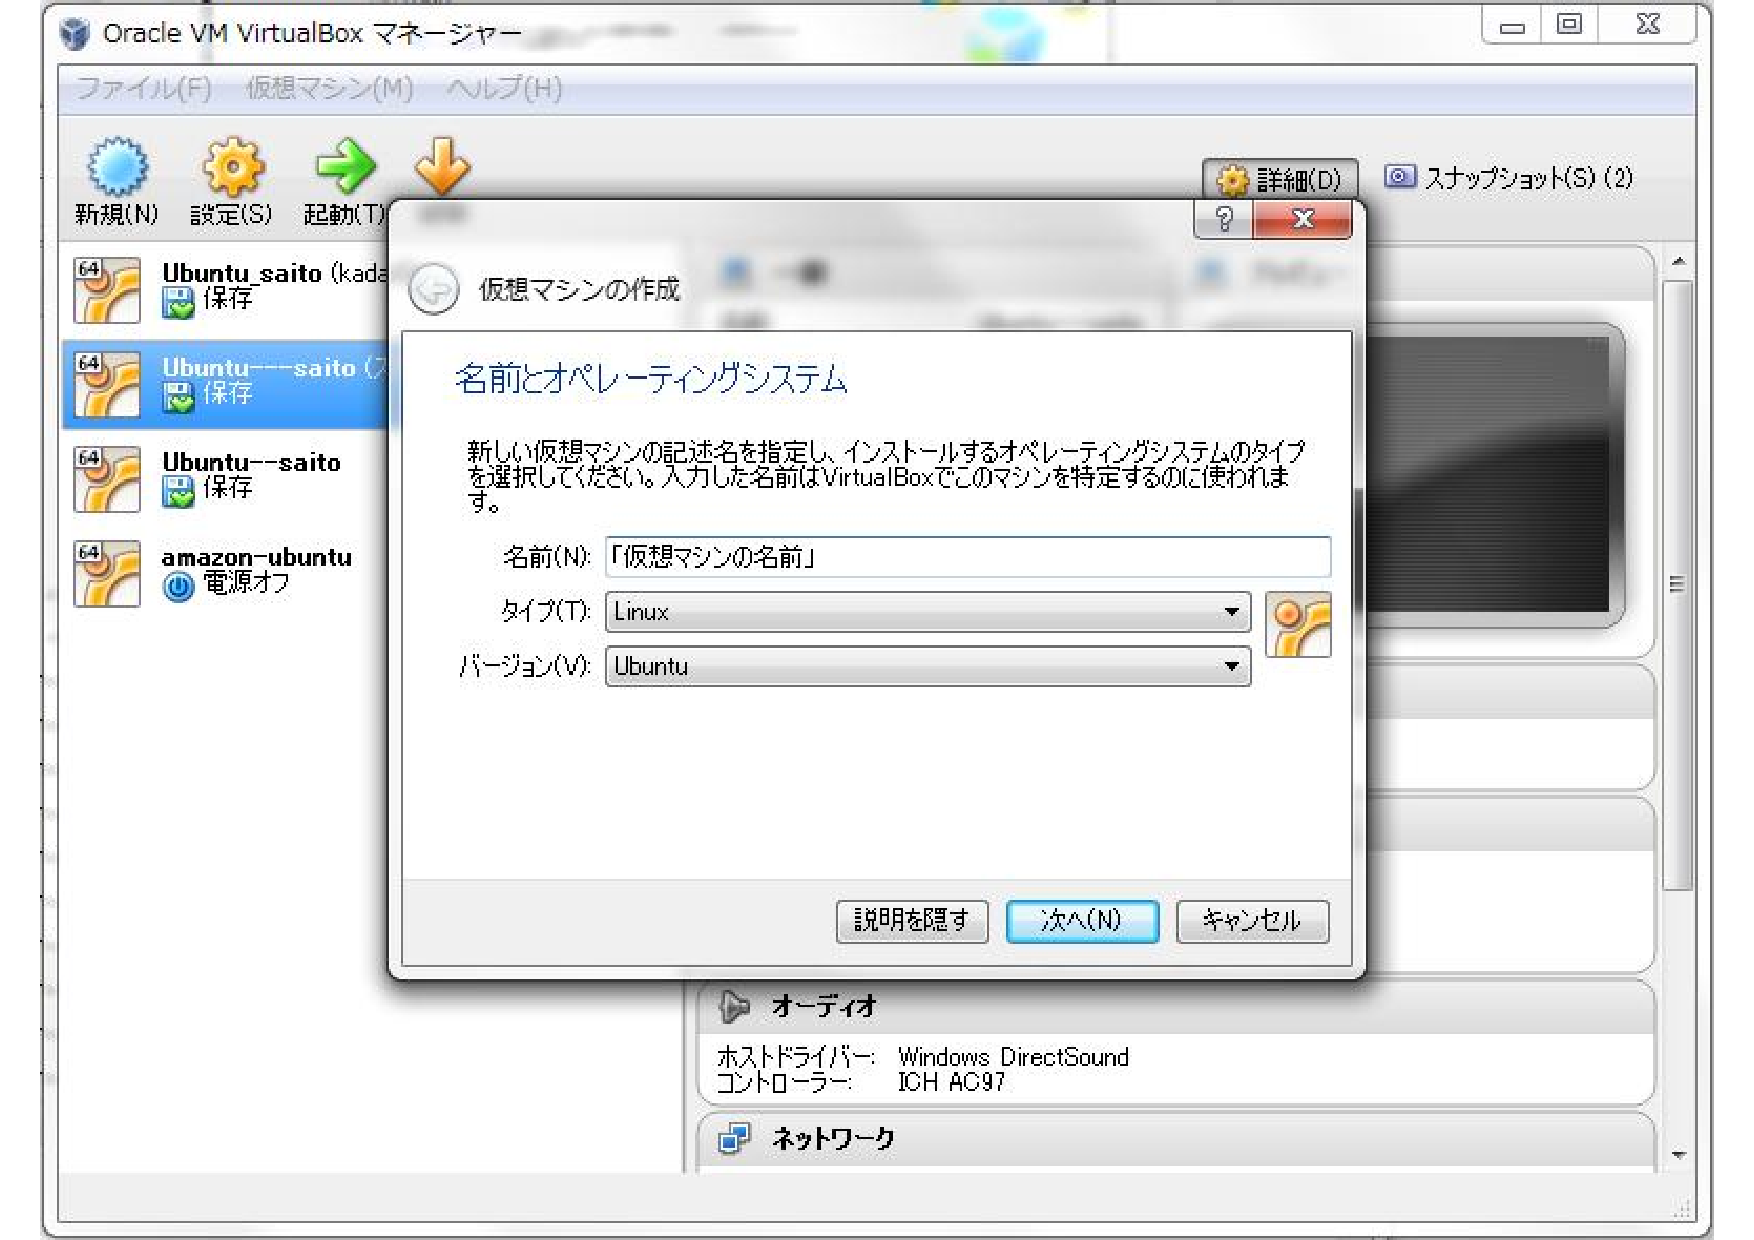
\includegraphics[width=8cm,clip]{VirtualBox2.pdf}
\caption{VirtualBoxでの仮想マシン作成}
\label{VirtualBoxinstall2}

\end{figure}

 \item 	「名前(N)」で仮想マシンの名前を設定する.「タイプ(T)」のOS選択でLinuxを選択し,「バージョン(V)」のLinuxの数ある派生先からUbuntuを選択する.

\begin{figure}[htbp]

\centering
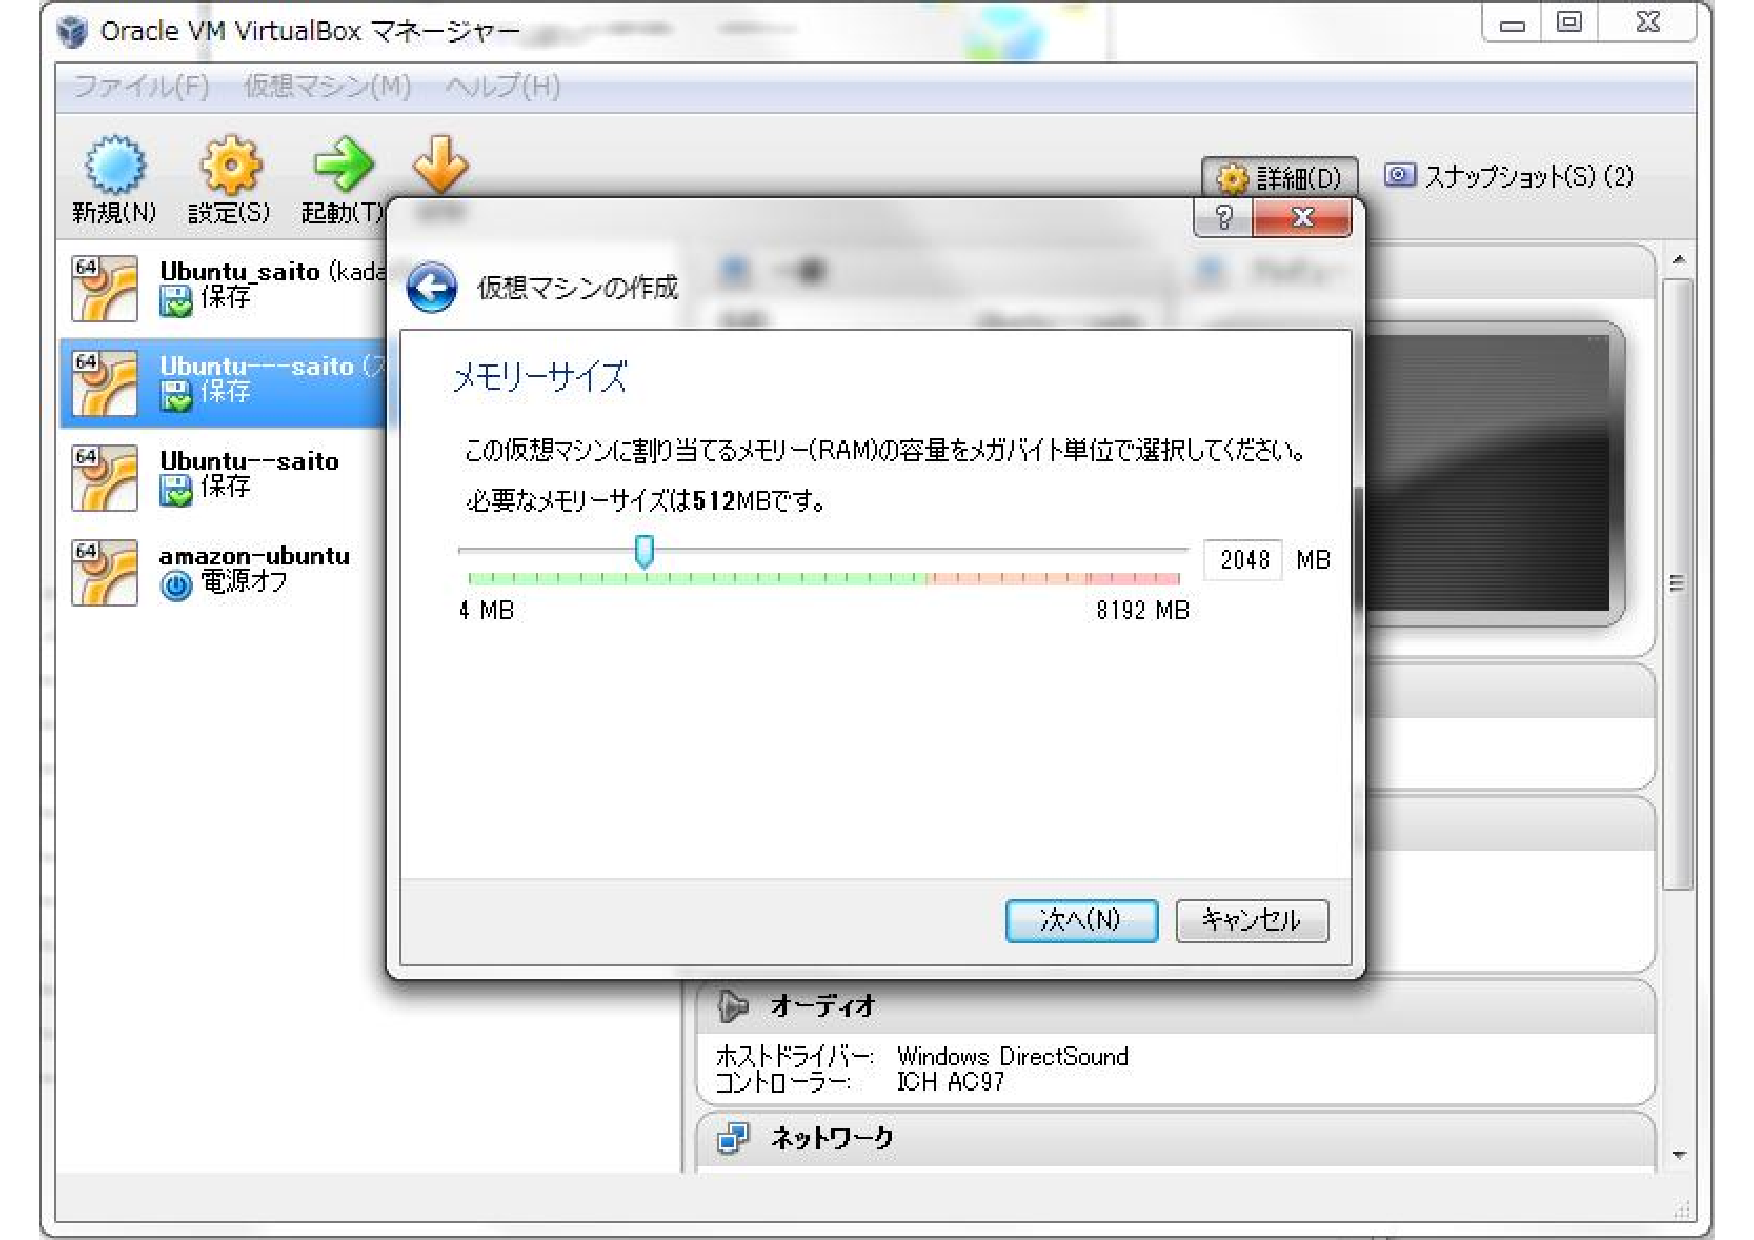
\includegraphics[width=8cm,clip]{VirtualBox3.pdf}
\caption{VirtualBoxでの仮想マシン作成}
\label{VirtualBoxinstall3}

\end{figure}

 \item 	生成させた仮想マシンを起動して,仮想DVDファイルディスクを選択する.

 \item 	ダウンロードしたUbuntu.isoを選択し,仮想マシンにUbuntuをインストールする.


\begin{figure}[htbp]

\centering
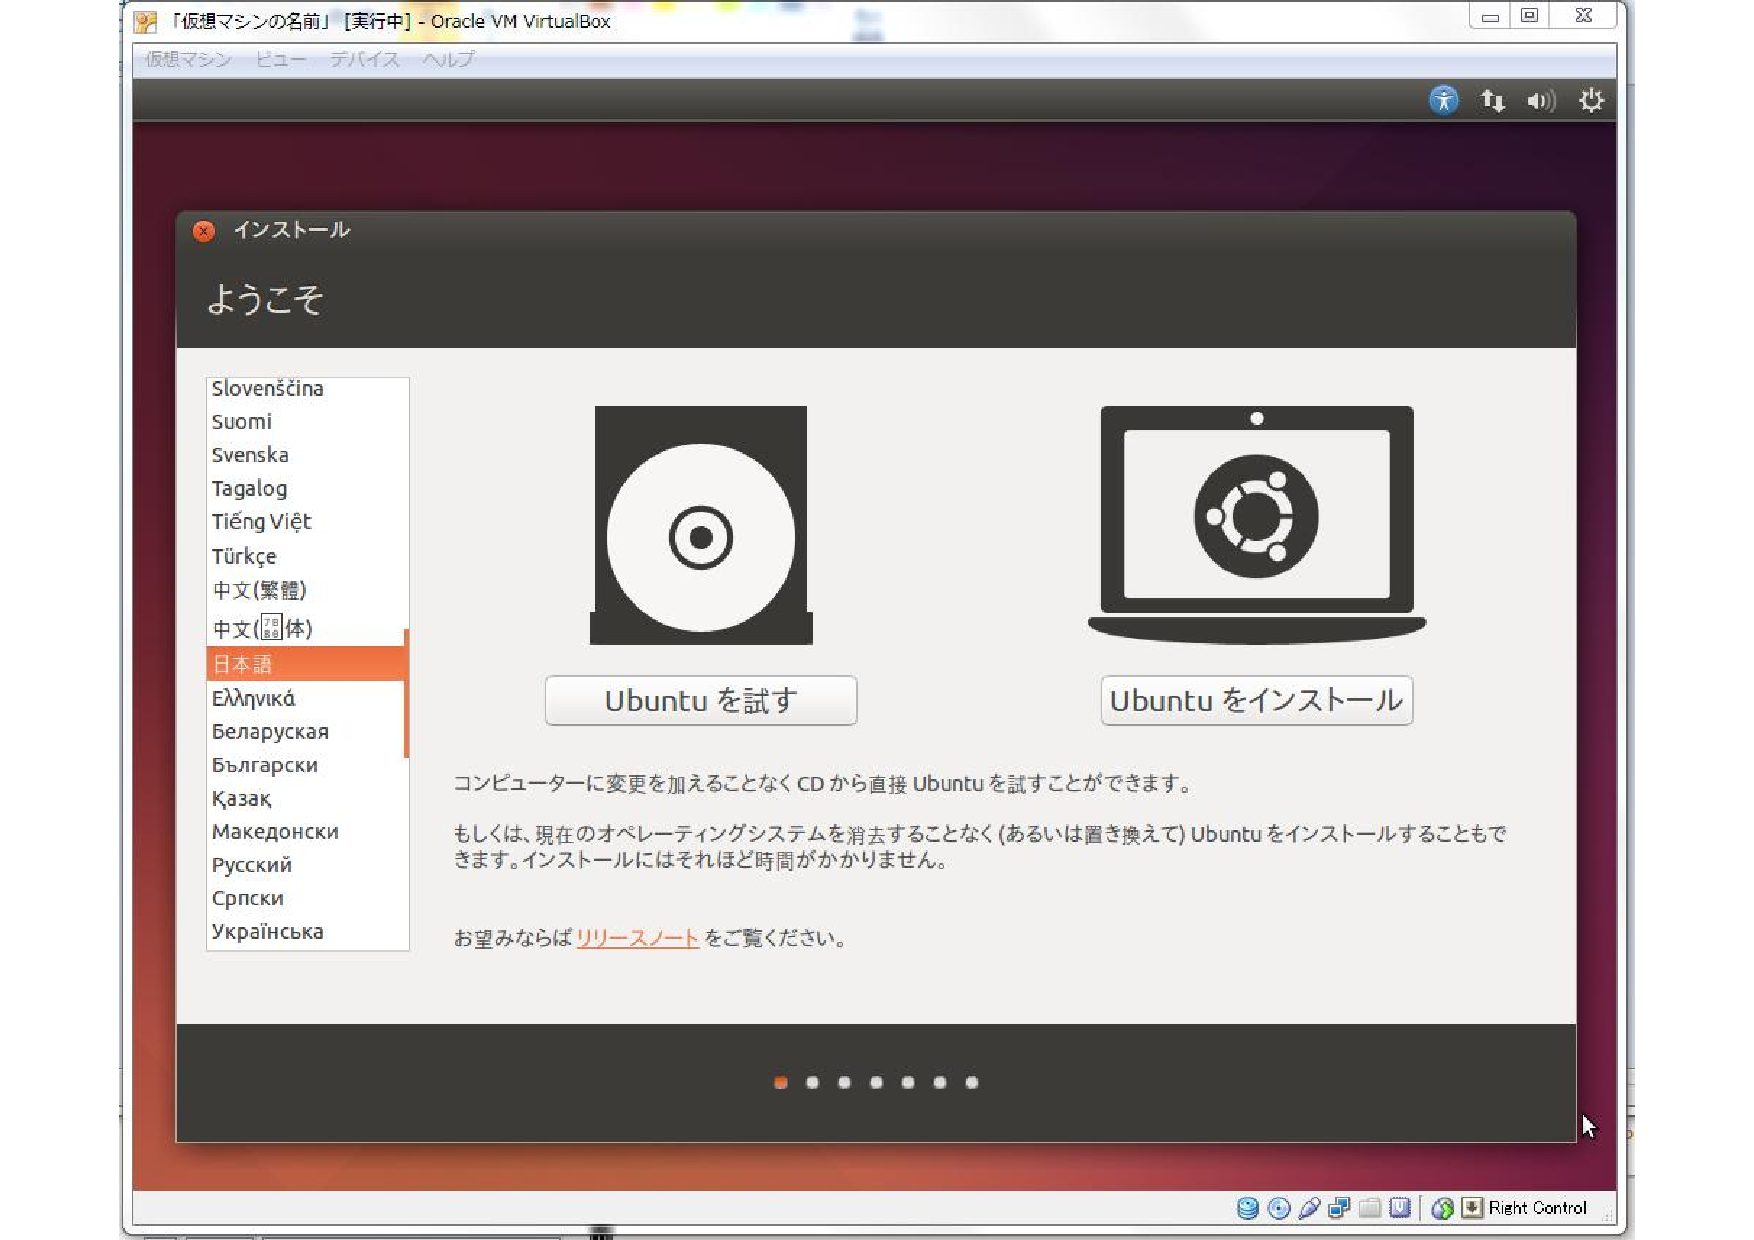
\includegraphics[width=8cm,clip]{Ubuntuinstall.pdf}
\caption{Ubuntuのインストール}
\label{Ubuntuinstall}

\end{figure}

\end{enumerate}



\subsection{NetBeansの導入}

NetBeansJAVAやPHPでのアプリケーション開発に対応した統合開発環境である.


\begin{enumerate}


 \item 	仮想マシン内で, url{https://netbeans.org/downloads/} NetBeansのサイトからNetBeansIDE8.1 (ダウンロードハンドルからすべてをクリック)をダウンロードする.

 \item 	ダウンロードが完了すればUbuntuから端末をクリックして,

{sh ~/netbeans-8.1-ml-linux.sh} 

というコマンドを実行しインストールができる.



\begin{figure}[htbp]

\centering
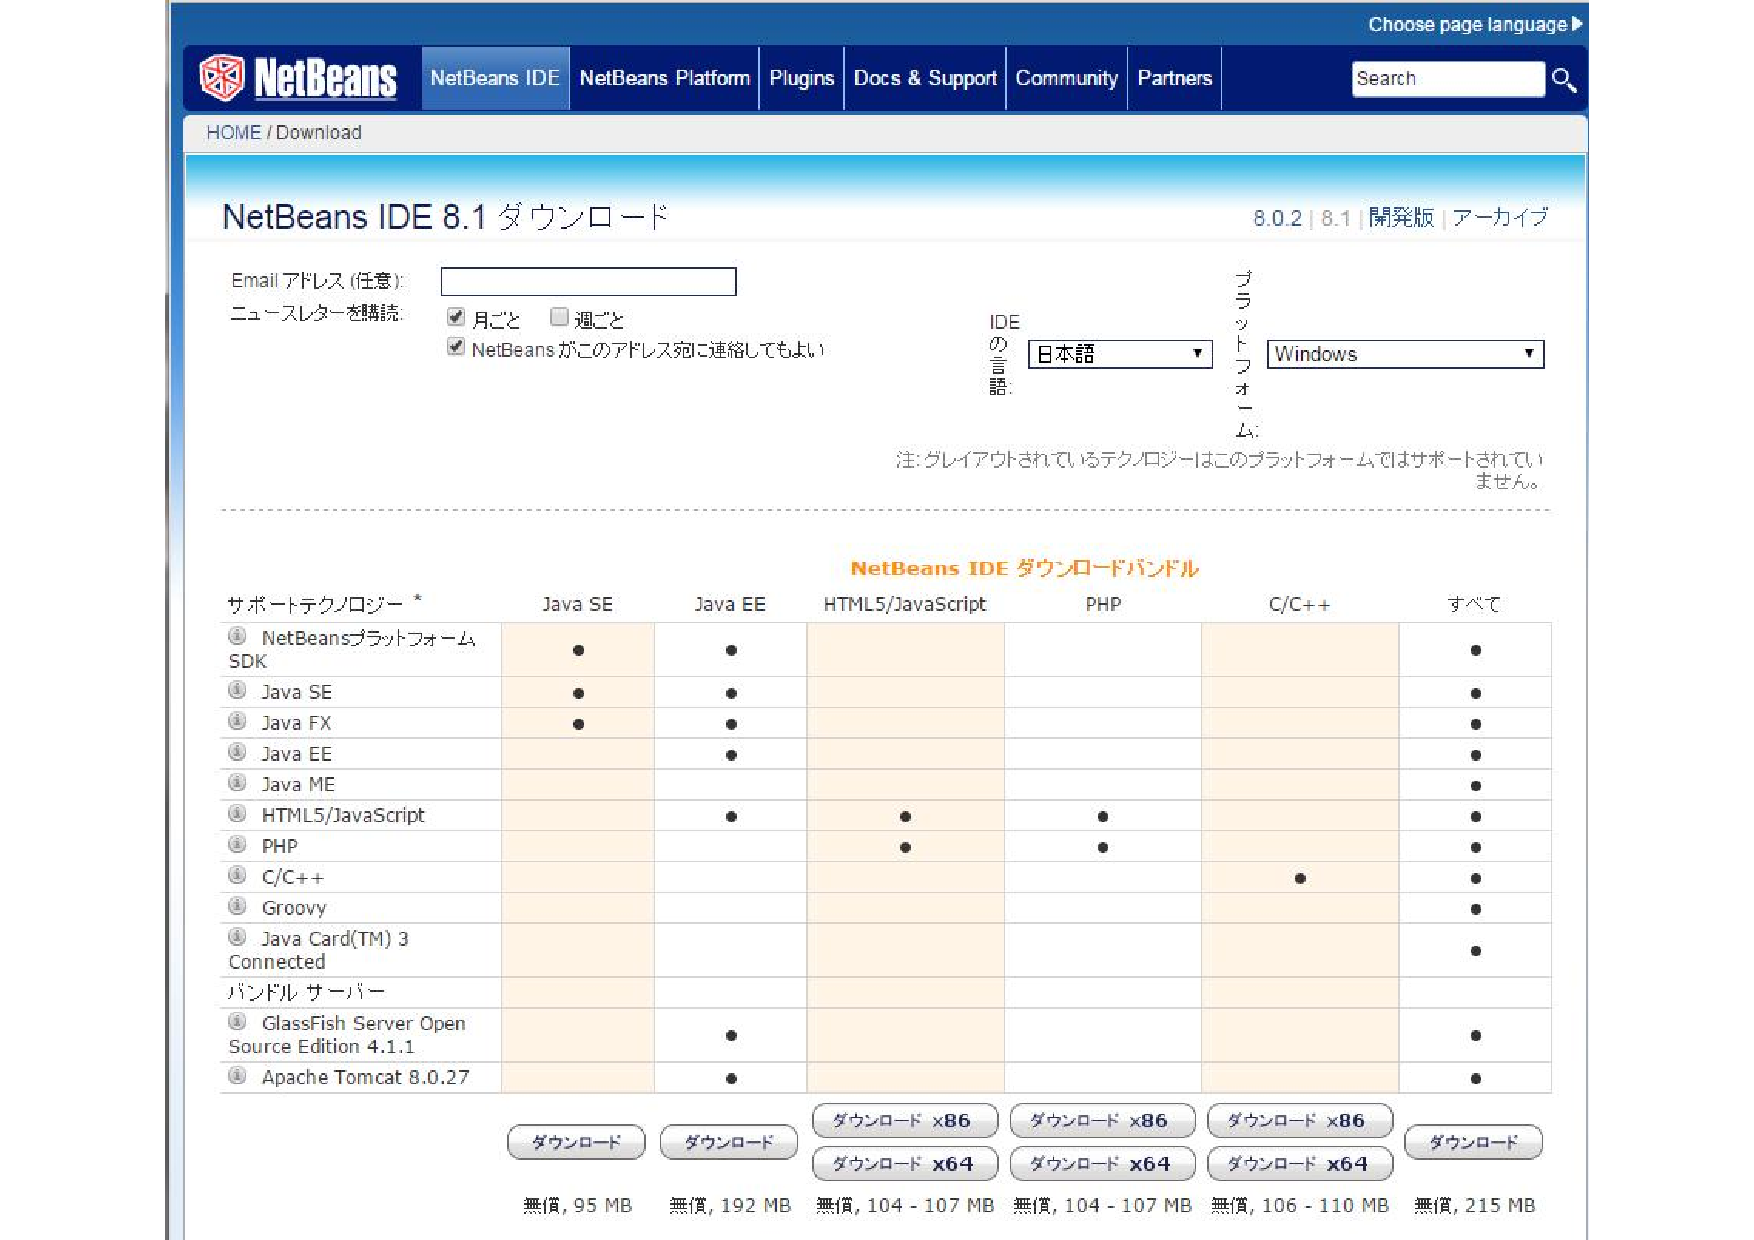
\includegraphics[width=8cm,clip]{NetBeans.pdf}
\caption{NetBeansのダウンロード}
\label{NetBeans}

\end{figure}


\end{enumerate}



\section{AmazonAPI}

Amazonでは「amazonProductAdvertisingAPI」というAmazonが提供するAPIがある.
このサービスを利用することでAmazonの商品データへのアクセスが可能となる.
ISBN,ASINに記載された商品データが分かるためそれを利用する予定とした.

\subsection{APIの運用,テスト}

矢吹准教授の協力により作成した,JAVAプログラムを使用し動作の確認をする.

利用するにあたりテストプログラムとして運用したものが下記にあたる.






\clearpage





\subsubsection{プログラム1}


\begin{lstlisting}

package com.amazon.associates.sample;

import java.util.*;

/**
 * 特定のアイテムについての情報をASINを指定して取得するためのURLを作る。
 *
 * @author yabuki
 */
public class Sample1 {

  public static void main(String[] args) throws Exception {
    String AssociateTag = "「AssociateTag名」";
    String asin = "「調べたいASINコード」";
    if (args.length != 0) {
      asin = args[0];
    }
    String Version = "2013-08-01";

    Map<String, String> params = new HashMap<>();
    params.put("AssociateTag", AssociateTag);
    params.put("Operation", "ItemLookup");
    params.put("ItemId", asin);
    params.put("ResponseGroup", "ItemAttributes,Reviews");//Reviewsリンクしか帰ってこないから意味なし
    params.put("Version", Version);
    SignedRequestsHelper instance = new SignedRequestsHelper();
    String apiUrl = instance.sign(params);
    System.out.println("APIのためのURL:\n" + apiUrl);
  }
}


\end{lstlisting}


\subsubsection{プログラム1について}

プログラム1はAssociateTag名とISBN,ASINを記入することで商品のReviewsリンクを参照するプログラムである.
この時点ではリンクの参照しか行えないため,レビューのリンクの場所は特定できたものの統計は参照できない.




\clearpage






\subsubsection{プログラム2}

\begin{lstlisting}
package com.amazon.associates.sample;

import java.util.*;
import java.net.*;
import javax.xml.xpath.*;
import org.w3c.dom.*;
import org.xml.sax.*;

/**
 * ASINで指定したアイテムの商品名をAPIで取得する。
 *
 * @author yabuki
 */
public class Sample2 {

  public static void main(String[] args) throws Exception {
    String AssociateTag = "「AssociateTag名」";
    String asin = "「調べたいASINコード」";
    if (args.length != 0) {
      asin = args[0];
    }
    String Version = "2013-08-01";

    Map<String, String> params = new HashMap<>();
    params.put("AssociateTag", AssociateTag);
    params.put("Operation", "ItemLookup");
    params.put("ItemId", asin);
    params.put("ResponseGroup", "ItemAttributes,Reviews");//Reviewsリンクしか帰ってこないから意味なし
    params.put("Version", Version);
    SignedRequestsHelper instance = new SignedRequestsHelper();
    String apiUrl = instance.sign(params);
    System.out.println("APIのためのURL:\n" + apiUrl);

    XPath xpath = XPathFactory.newInstance().newXPath();
    String expression = "//*[namespace-uri() = 'http://webservices.amazon.com/AWSECommerceService/" + Version + "'][local-name() = 'Title']";

    URL url = new URL(apiUrl);
    HttpURLConnection connection = (HttpURLConnection) url.openConnection();
    InputSource is = new InputSource(connection.getInputStream());
    Node node = (Node) xpath.evaluate(expression, is, XPathConstants.NODE);
    String title = node.getTextContent();
    System.out.println("Title:\n" + title);
  }

}

\end{lstlisting}



\subsubsection{プログラム2について}

プログラム2はAssociateTag名とISBN,ASINを記入することでXML形式のURLを取得できる.
ここからXMLのデータから取り出しを行うことで一部のほしい情報のみを取得することができる.

\subsection{クローラーの利用}

1プログラム2についてはさらに追記を行うことでAPIでのレビューデータの取得が可能となるが,HTTPクライアントで記述することでAPIを使わずにレビューデータを取得することができ,Amazonのレビューページは「http://www.amazon.co.jp/product-reviews/ISBN,ASINコード/」のURLで成り立っていることが判明した.URLの参照に手間がかからずレビューデータは
よって,こちらの方法はこの時点でAPIの使用を止め,クローラーを利用することとした.


\section{クロームを利用したレビューデータ収集}

「http://www.amazon.co.jp/product-reviews/ISBN,ASIN/」でAmazonの商品ページのURLが構成されていることが分かった.

この性質を利用して調べたい対象のISBN,ASINを記入することで対象のサイトにアクセスすることができる.
html内の文章でレビューデータの共通項目として「○○人中○人が」,「5つ星のうち○」(○内には1~9の数値のいずれかが当てはまる)との記述があるのでクロームでは正規表現を用いてその文字を参照し,一商品あたりのすべてのレビューデータを集めていく.



\subsubsection{プログラム3}

\begin{lstlisting}
package com.amazon.associates.sample;

import java.net.*;
import java.util.regex.*;
import org.apache.commons.io.*;

/**
 * ASINで指定したアイテムのレビューを取得する。(1ページ限定)
 * 
 * @author yabuki
 */
public class Sample3 {

  public static void main(String[] args) throws Exception {
    String asin = "「調べたいASINコード」"
    if (args.length != 0) {
      asin = args[0];
    }
    String charset = "Shift_JIS"; //驚くところ!
    String urlStr = "http://www.amazon.co.jp/product-reviews/" + asin + "/";
    //String urlStr = "http://www.amazon.co.jp/product-reviews/4873115655?pageNumber=2";//テスト用
    URL url = new URL(urlStr);
    HttpURLConnection connection = (HttpURLConnection) url.openConnection();
    System.err.printf("%s %s\n", connection.getResponseCode(), connection.getResponseMessage());
    String responseBody = IOUtils.toString(connection.getInputStream(), charset).replace("\n", "");//改行削除

    Pattern pattern1 = Pattern.compile("([0-9]*)\\s*人中、([0-9]*)\\s*人の方が.*?5つ星のうち\\s*([0-9|\\.]*)");
    Pattern pattern2 = Pattern.compile("5つ星のうち\\s*([0-9|\\.]*)");

    //1件目は平均
    for (String aReview : responseBody.split("<!-- BOUNDARY -->")) {
      Matcher matcher1 = pattern1.matcher(aReview);
      int people = 0;
      int helpful = 0;
      double star = 0;
      if (matcher1.find()) {
        people = Integer.parseInt(matcher1.group(1));
        helpful = Integer.parseInt(matcher1.group(2));
        star = Double.parseDouble(matcher1.group(3));
        System.out.printf("星%f。%d人中%d人が参考になった。\n", star, people, helpful);
      } else {
        Matcher matcher2 = pattern2.matcher(aReview);
        if (matcher2.find()) {
          star = Double.parseDouble(matcher2.group(1));
          System.out.printf("星%f。\n", star);
        }
      }
    }
  }
}

\end{lstlisting}


\subsubsection{プログラム3について}

プログラム3はISBN,ASINに記入した商品の1ページのみのレビューデータの取得が可能である.

1ページのみであるが,平均評価,レビューの回覧数,レビューが参考になったと答えた人数を取得することができる.


\subsubsection{プログラム4}

\begin{lstlisting}
package com.amazon.associates.sample;

import java.net.*;
import java.util.*;
import java.util.regex.*;
import org.apache.commons.io.*;

/**
 * ASINで指定したアイテムのレビューを取得・記憶し、重み付き評価値を求める。(1ページ限定)
 * 
 * @author yabuki
 */
public class Sample4 {

  public static void main(String[] args) throws Exception {
    String asin = "「調べたいASINコード」"
    if (args.length != 0) {
      asin = args[0];
    }
    String charset = "Shift_JIS"; //驚くところ!
    String urlStr = "http://www.amazon.co.jp/product-reviews/" + asin + "/";
    //String urlStr = "http://www.amazon.co.jp/product-reviews/4873115655?pageNumber=2";//テスト用
    URL url = new URL(urlStr);
    HttpURLConnection connection = (HttpURLConnection) url.openConnection();
    System.err.printf("%s %s\n", connection.getResponseCode(), connection.getResponseMessage());
    String responseBody = IOUtils.toString(connection.getInputStream(), charset).replace("\n", "");//改行削除

    Pattern pattern1 = Pattern.compile("([0-9]*)\\s*人中、([0-9]*)\\s*人の方が.*?5つ星のうち\\s*([0-9|\\.]*)");
    Pattern pattern2 = Pattern.compile("5つ星のうち\\s*([0-9|\\.]*)");

    List<Review> reviews = new LinkedList<>();
    for (String aReview : responseBody.split("<!-- BOUNDARY -->")) {
      Matcher matcher1 = pattern1.matcher(aReview);
      int people = 0;
      int helpful = 0;
      double star = 0;
      if (matcher1.find()) {
        people = Integer.parseInt(matcher1.group(1));
        helpful = Integer.parseInt(matcher1.group(2));
        star = Double.parseDouble(matcher1.group(3));
        reviews.add(new Review(star, people, helpful, 1));
      } else {
        Matcher matcher2 = pattern2.matcher(aReview);
        if (matcher2.find()) {
          star = Double.parseDouble(matcher2.group(1));
          reviews.add(new Review(star, people, helpful, 1));
        }
      }
    }
    System.out.println("平均スター(ウェブ上):" + reviews.get(0));//1件目は平均
    reviews.remove(0);
    if (responseBody.contains("評価が高い有用性のあるレビュー")) {//最初の2件は重複
      reviews.remove(0);
      reviews.remove(0);
    }

    double totalStar = 0;//星の総数
    double totalStarWeighted = 0;//星の重み付き総数
    double totalWeight = 0;//重み
    for (Review r : reviews) {
      System.out.println(r);
      double star = r.getStar();
      totalStar += star;
      int people = r.getPeople();
      if (people != 0) {//評価のあるレビューのみ
        double weight = 1.0 * r.getHelpful() / people;
        totalStarWeighted += star * weight;
        totalWeight += weight;
      }
    }
    int numReviews = reviews.size();
    System.out.println("レビュアー数:" + numReviews);
    System.out.println("平均スター(計算結果):" + totalStar / numReviews);
    System.out.println("平均スター(重み付き)" + totalStarWeighted / totalWeight);
  }
}

\end{lstlisting}

\subsubsection{プログラム4について}

プログラム4はISBN,ASINに記入した商品の1ページのみのレビューデータの取得が可能である.
1ページのみであるが,平均評価,レビューの回覧数,レビューが参考になったと答えた人数,\ref{hyoukahouhou} にて説明した,レビューの回覧数にレビューが参考になったと答えた人数を割った数に
評価をかけた「重み付き評価」を取得することができる.




\subsubsection{プログラム5}

\begin{lstlisting}

package com.amazon.associates.sample;

import java.io.*;
import java.net.*;
import java.util.*;
import java.util.regex.*;
import org.apache.commons.io.*;

/**
 * ASINで指定したアイテムのレビューを取得・記憶し、重み付き評価値を求める。(複数ページ対応)
 * 
 * @author yabuki
 */
public class Sample5 {

  static List<Review> extractReviews(String urlStr, int page) throws MalformedURLException {
    try {
      String charset = "Shift_JIS"; //驚くところ!
      System.err.println(urlStr);

      URL url = new URL(urlStr);
      HttpURLConnection connection;
      connection = (HttpURLConnection) url.openConnection();
      System.err.printf("%s %s\n", connection.getResponseCode(), connection.getResponseMessage());
      String responseBody = IOUtils.toString(connection.getInputStream(), charset).replace("\n", "");//改行削除

      Pattern pattern1 = Pattern.compile("([0-9]*)\\s*人中、([0-9]*)\\s*人の方が.*?5つ星のうち\\s*([0-9|\\.]*)");
      Pattern pattern2 = Pattern.compile("5つ星のうち\\s*([0-9|\\.]*)");

      List<Review> reviews = new LinkedList<>();
      for (String aReview : responseBody.split("<!-- BOUNDARY -->")) {
        Matcher matcher1 = pattern1.matcher(aReview);
        int people = 0;
        int helpful = 0;
        double star = 0;
        if (matcher1.find()) {
          people = Integer.parseInt(matcher1.group(1));
          helpful = Integer.parseInt(matcher1.group(2));
          star = Double.parseDouble(matcher1.group(3));
          reviews.add(new Review(star, people, helpful, page));
        } else {
          Matcher matcher2 = pattern2.matcher(aReview);
          if (matcher2.find()) {
            star = Double.parseDouble(matcher2.group(1));
            reviews.add(new Review(star, people, helpful, page));
          }
        }
      }
      if (page == 1) {
        System.out.println("平均スター(ウェブ上):" + reviews.get(0));//1件目は平均
      }
      reviews.remove(0);
      if (responseBody.contains("評価が高い有用性のあるレビュー")) {//最初の2件は重複
        reviews.remove(0);
        reviews.remove(0);
      }

      //次のページがあるか
      Pattern pattern3 = Pattern.compile("<a href=\"([^\\\"]*?)\">次へ");
      Matcher matcher3 = pattern3.matcher(responseBody);
      if (matcher3.find()) {
        String nextPageUrlStr = matcher3.group(1);
        reviews.addAll(extractReviews(nextPageUrlStr, page + 1));
      }
      return reviews;
    } catch (IOException ex) {//エラーが発生したら、5秒Sleepしてやり直す
      System.err.println(ex.getLocalizedMessage());
      try {
        Thread.sleep(5000);
      } catch (InterruptedException e) {
      }
      return extractReviews(urlStr, page);
    }

  }

  public static void main(String[] args) throws Exception {
    String asin = "4274065979";//ハッカーと画家 コンピュータ時代の創造者たち
    //String asin = "B00IFTTOAK";//マリオカート8
    if (args.length != 0) {
      asin = args[0];
    }
    String urlStr = "http://www.amazon.co.jp/product-reviews/" + asin + "/";
    List<Review> reviews = new LinkedList<>();
    reviews.addAll(extractReviews(urlStr, 1));

    double totalStar = 0;//星の総数
    double totalStarWeighted = 0;//星の重み付き総数
    double totalWeight = 0;//重み
    int numReviewsPage1 = 0;//1ページ目のレビュアー数
    double totalStarPage1 = 0;//1ページ目の星の総数
    double totalStarWeightedPage1 = 0;//1ページ目の星の重み付き総数
    double totalWeightPage1 = 0;//1ページ目の重み
    for (Review r : reviews) {
      System.out.println(r);
      double star = r.getStar();
      totalStar += star;
      int page = r.getPage();
      if (page == 1) {
        ++numReviewsPage1;
        totalStarPage1 += star;
      }
      int people = r.getPeople();
      if (people != 0) {
        double weight = 1.0 * r.getHelpful() / people;
        totalStarWeighted += star * weight;
        totalWeight += weight;
        if (page == 1) {
          totalStarWeightedPage1 += star * weight;
          totalWeightPage1 += weight;

        }
      }
    }
    int numReviews = reviews.size();
    System.out.println("レビュアー数:" + numReviews);
    System.out.println("平均スター(計算結果):" + totalStar / numReviews);
    System.out.println("平均スター(1ページ目):" + totalStarPage1 / numReviewsPage1);
    System.out.println("平均スター(重み付き)" + totalStarWeighted / totalWeight);
    System.out.println("平均スター(1ページ目・重み付き)" + totalStarWeightedPage1 / totalWeightPage1);

  }
}


\end{lstlisting}


\subsubsection{プログラム5について}

プログラム5はISBN,ASINに記入した商品のすべてのレビューデータの取得が可能である.
このプログラムで一つのISBN,ASINにおけるすべてのページの平均評価,レビューの回覧数,レビューが参考になったと答えた人数,\ref{hyoukahouhou} にて説明した,レビューの回覧数にレビューが参考になったと答えた人数を割った数に評価をかけた「重み付き評価」を取得することができる.



\section{エクセルを利用したレビューデータ収集}
判断材料を増やす試みを行った結果,プログラムの改変に多大な時間を要することとなったので手作業で数値の入力をし,エクセルで統計を取ることとした.



\subsection{レビューの入力場所,収集項目の計算}

\begin{figure}[htbp]

\centering
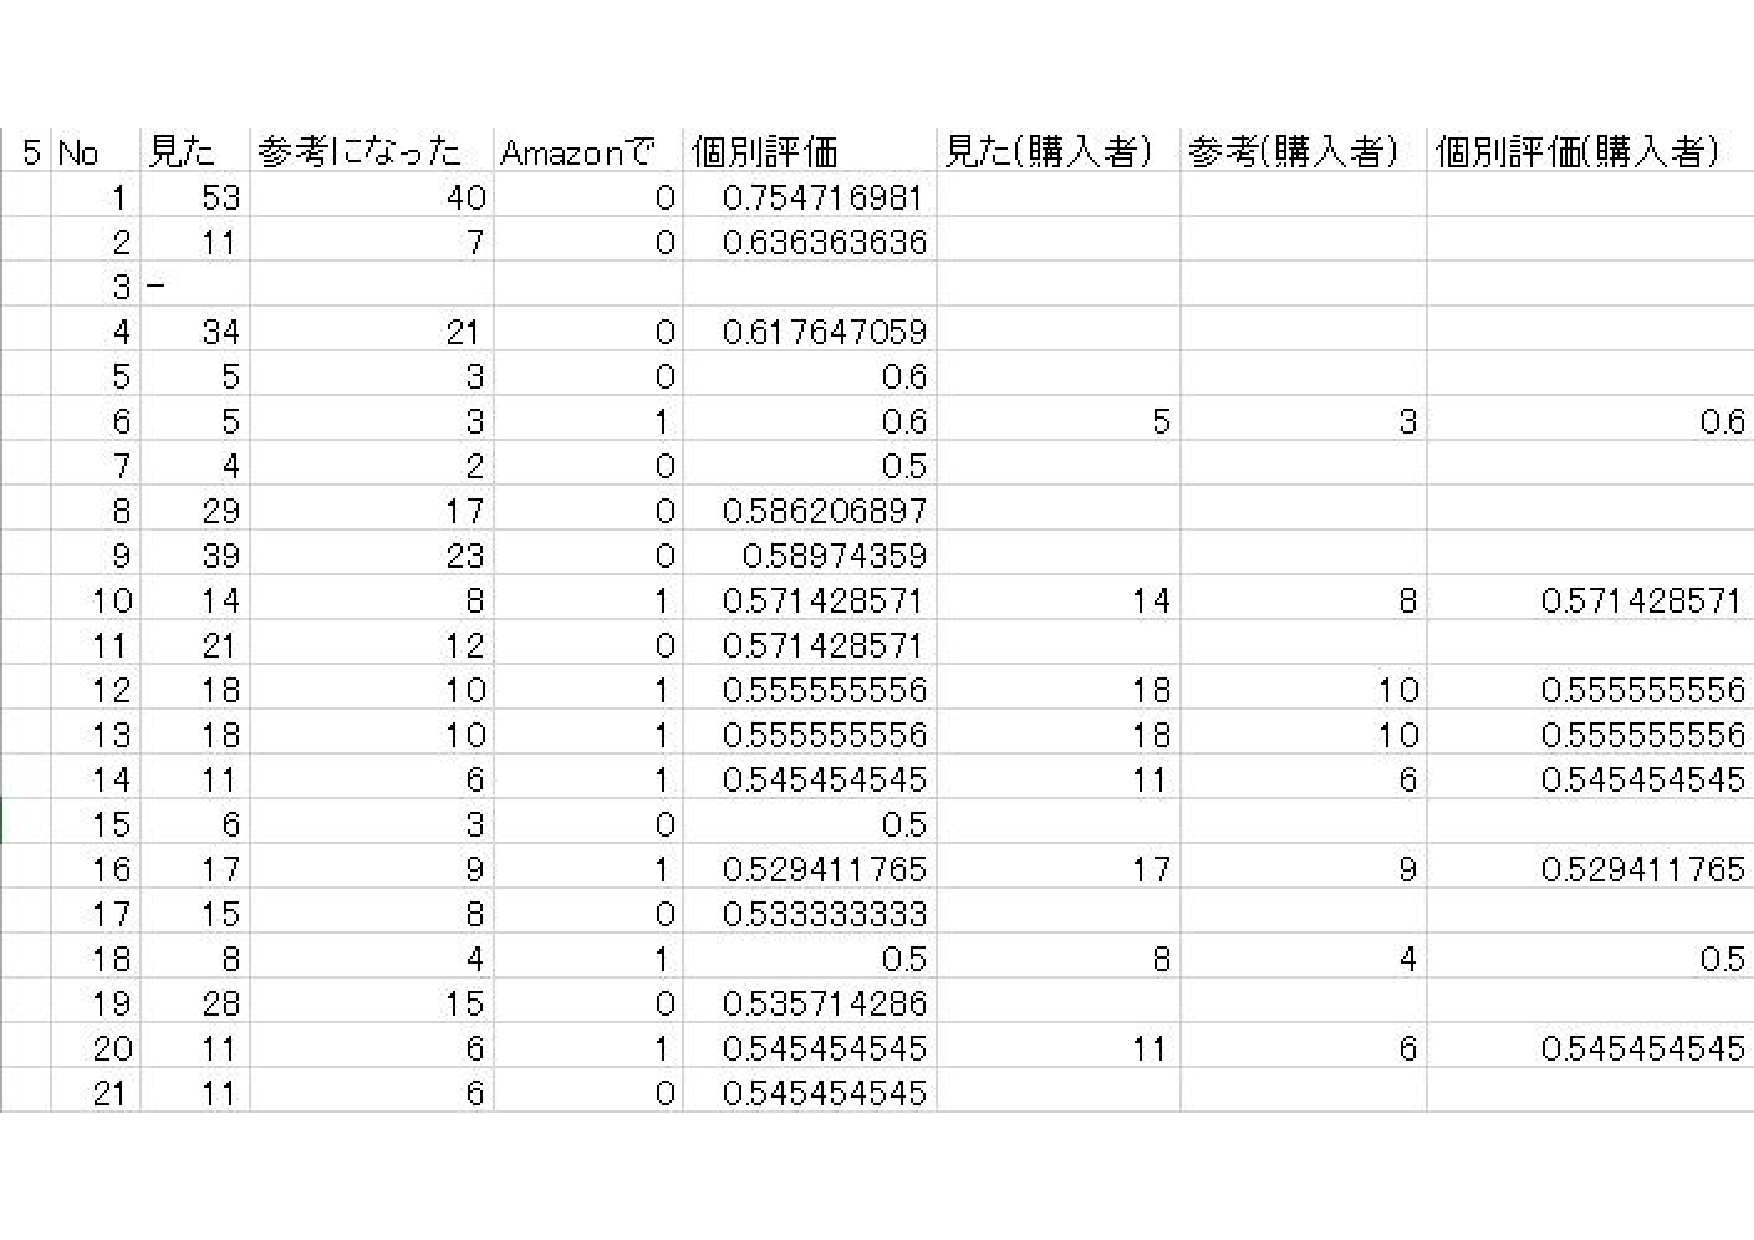
\includegraphics[width=12cm,clip]{ekuseru.pdf}
\caption{レビューの入力場所,収集項目の計算}
\label{ekuseru}

\end{figure}

\subsection{レビューの入力場所}

「見た」が記入されている列にレビューを見た人数,「参考になった」が記入されている列にレビューが参考になったと答えた人数,「Amazonで」が記入されている列にAmazonで購入されていた場合は1をそうでない場合は0をを入力します.これらを評価段階1-5で分けられたページごとに記入していきます.

\subsection{収集項目の計算}

\begin{itemize}
\setlength{\parskip}{3mm}

 \item	{=IF(ISBLANK(D2),"",D2/C2)}と入力することで,レビューが参考になったと答えた人数からレビューを見た人数を割った個別評価が出力されることとなり,空白の場合は結果が出ず空白が出力される式ができます.


 \item	{=IF(E2=1,OFFSET(E2,0,-2),"")}と入力することで,Amazonで購入した人のレビューを見た人である場合その場所に出力できます.

 \item	{=IF(E2=1,OFFSET(E2,0,-1),"")}と入力することで,Amazonで購入した人のレビューを参考になったと答えた場合その場所に出力できます.

 \item	{=IF(E2=1,OFFSET(E2,0,1),"")}と入力することで,Amazonで購入した人の個別評価をその場所に出力できます.


\end{itemize}


\subsection{収集したデータの統計}

このように収集したページごとに出力したデータをまとめ,割ることで重み付き評価が分かります.


\begin{figure}[htbp]

\centering
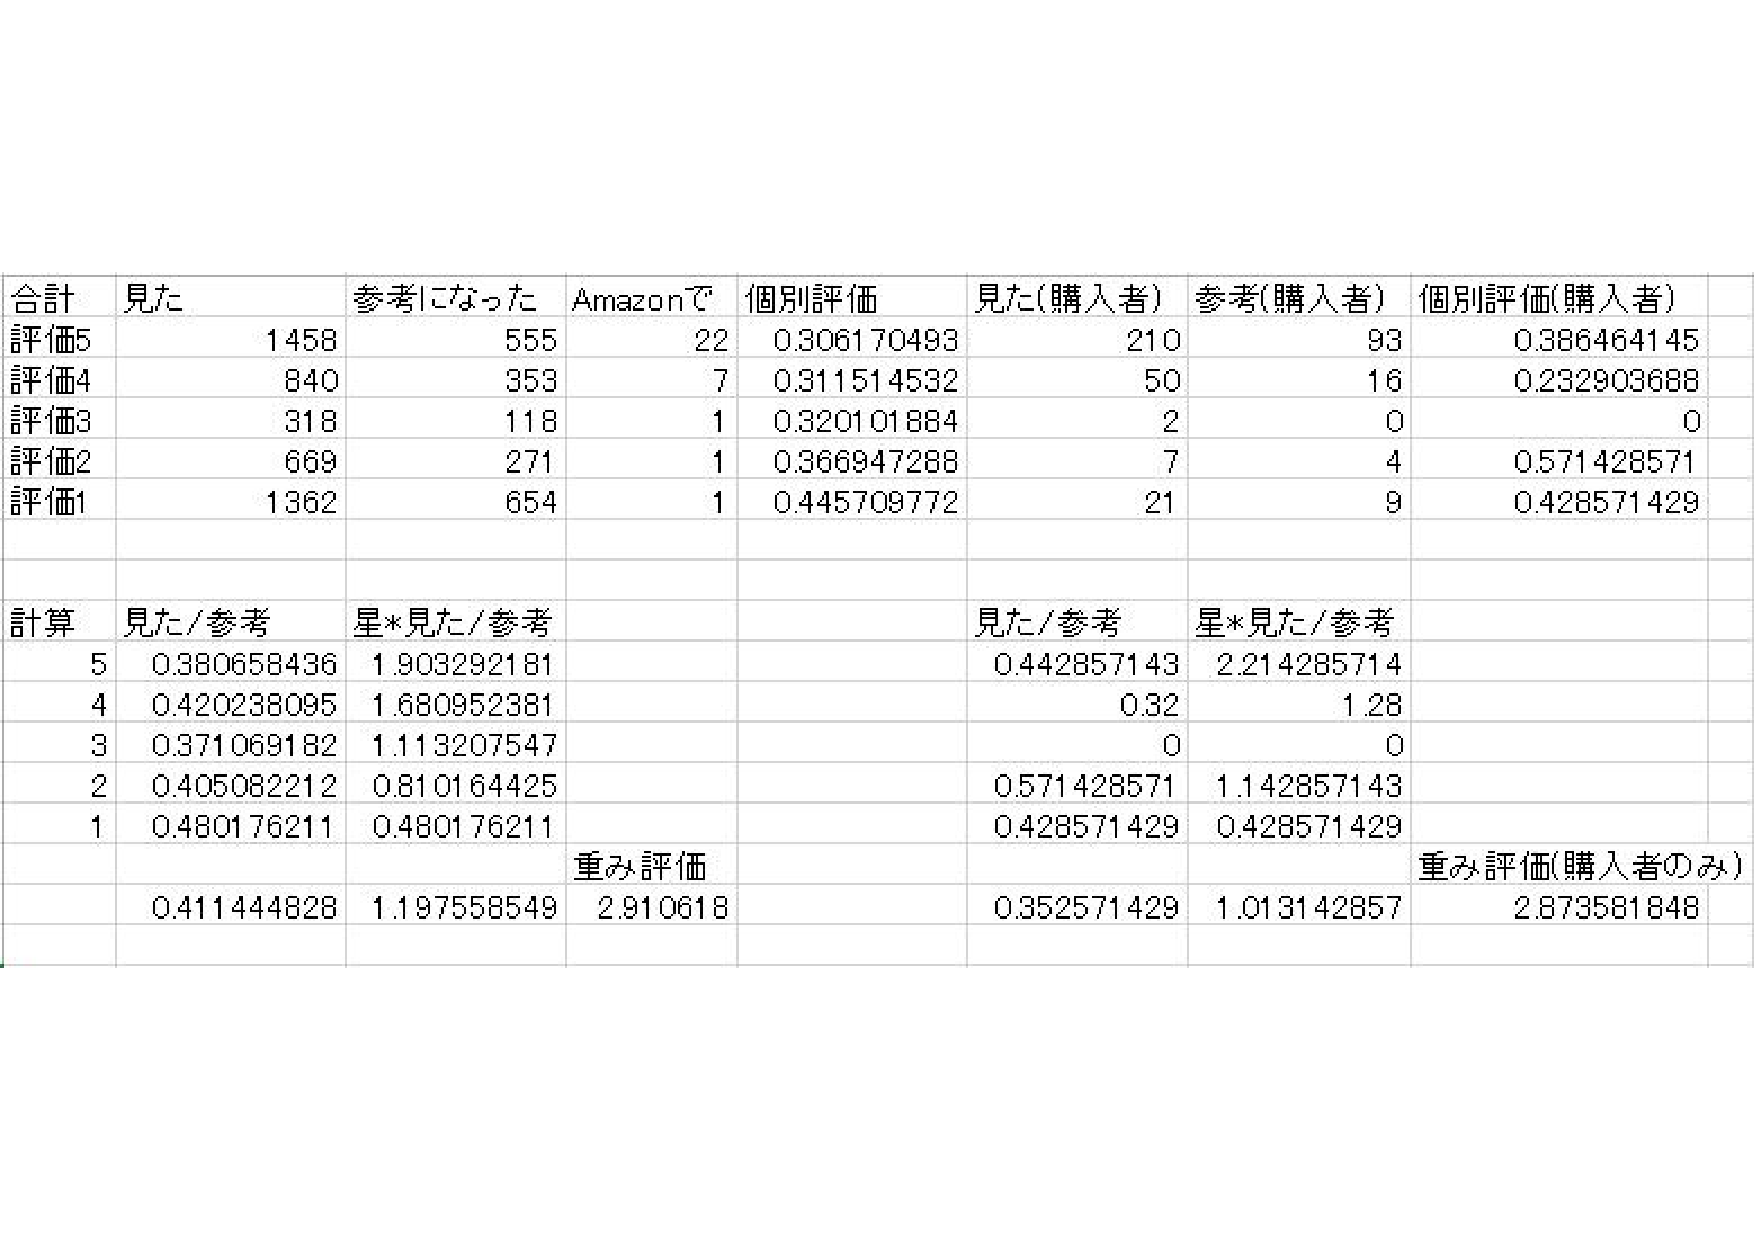
\includegraphics[width=12cm,clip]{ekuseru2.pdf}
\caption{収集したデータの統計}
\label{ekuseru2}

\end{figure}

\chapter{結果}

クローラーで87件,エクセルの手動で9件収集した.

\section{平均評価と重み付き評価の収集}



計86件のレビューデータをクローラーで収集した.

収集した項目は,平均評価,重み付き評価,の二種である.

評価数値は1~5の間で評価されている.




\begin{table}[htb]
\label{reviewtoukei}
  \begin{center}
    \caption{レビューデータ統計}


\begin{tabular}{|r|r|r|}

\hline
件数 & 平均評価 & 重み付き評価 \\
\hline\hline

1 &3.852 &3.623\\
2 &4.115 &4.016\\
3 &3.55 &3.218\\
4 &3.822 &3.765\\
5 &3.844 &3.319\\
6 &3.994 &4.077\\
7 &3.76 &3.75\\
8 &3.844 &3.319\\
9 &3.358 &2.891\\
10 &4.201 &4.337\\
11 &3.657 &3.476\\
12 &3.746 &3.195\\
13 &4.424 &4.359\\
14 &3.844 &3.319\\
15 &4.222 &4.236\\
16 &4.049 &4.171\\
17 &3.819 &3.36\\
18 &4.066 &3.823\\
19 &4.301 &4.434\\

	\hline
    \end{tabular}
  \end{center}
\end{table}



\clearpage





\begin{table}[htb]
\label{reviewtoukei2}
  \begin{center}
    \caption{レビューデータ統計2}


\begin{tabular}{|r|r|r|}

\hline
件数 & 平均評価 & 重み付き評価 \\
\hline\hline

21 &3.83 &3.523\\
22 &3.805 &3.127\\
23 &3.99 &4.079\\
24 &4.131 &4.112\\
25 &4.006 &4.014\\
26 &4.183 &4.067\\
27 &3.661 &3.523\\
28 &3.661 &3.523\\
29 &3.651 &3.521\\
30 &3.661 &3.523\\
31 &3.661 &3.523\\
32 &4.04 &3.887\\
33 &4.409 &4.359\\
34 &3.902 &3.769\\
35 &4.183 &4.067\\
36 &3.799 &3.726\\
37 &4.224 &4.29\\
38 &4.291 &4.446\\
39 &3.772 &4.056\\
40 &4.383 &4.005\\
41 &2.211 &1.561\\
42 &4.484 &4.523\\
43 &3.766 &3.583\\
44 &3.236 &2.897\\
45 &4.398 &4.453\\
46 &4.546 &4.527\\
47 &4.487 &4.661\\
48 &4.125 &4.226\\
49 &4.3 &4.458\\
50 &1.789 &1.289\\
51 &4.65 &4.83\\
52 &4.289 &4.313\\
53 &3.627 &3.745\\
54 &3.166 &2.625\\
55 &4.25 &4.274\\
56 &3.885 &3.749\\
57 &4.272 &4.352\\
58 &4.052 &4.13\\
59 &4.108 &4.356\\
60 &4.053 &4.061\\


	\hline
    \end{tabular}
  \end{center}
\end{table}


\clearpage




\begin{table}[htb]
\label{reviewtoukei3}
  \begin{center}
    \caption{レビューデータ統計3}


\begin{tabular}{|r|r|r|}

\hline
件数 & 平均評価 & 重み付き評価 \\
\hline\hline

61 &4.02 &4.039\\
62 &2.852 &2.392\\
63 &4.363 &4.634\\
64 &3.322 &3.22\\
65 &4.611 &4.689\\
66 &4.727 &4.851\\
67 &4.6 &4.764\\
68 &4.638 &4.842\\
69 &4.569 &4.639\\
70 &4.555 &4.815\\
71 &4.807 &4.892\\
72 &4.469 &4.59\\
73 &4.485 &4.575\\
74 &4.793 &4.761\\
75 &4.45 &4.732\\
76 &4.717 &4.822\\
77 &3.851 &3.578\\
78 &4.593 &4.809\\
79 &3.728 &3.675\\
80 &4.129 &3.946\\
81 &4.652 &4.823\\
82 &4.675 &4.824\\
83 &1.867 &1.687\\
84 &1.728 &1.381\\
85 &2.848 &2.637\\
86 &3.815 &3.572\\
87 &3.598 &3.14\\

	\hline
    \end{tabular}
  \end{center}
\end{table}



\clearpage

\subsection{分析結果}

\begin{figure}[htbp]

\centering
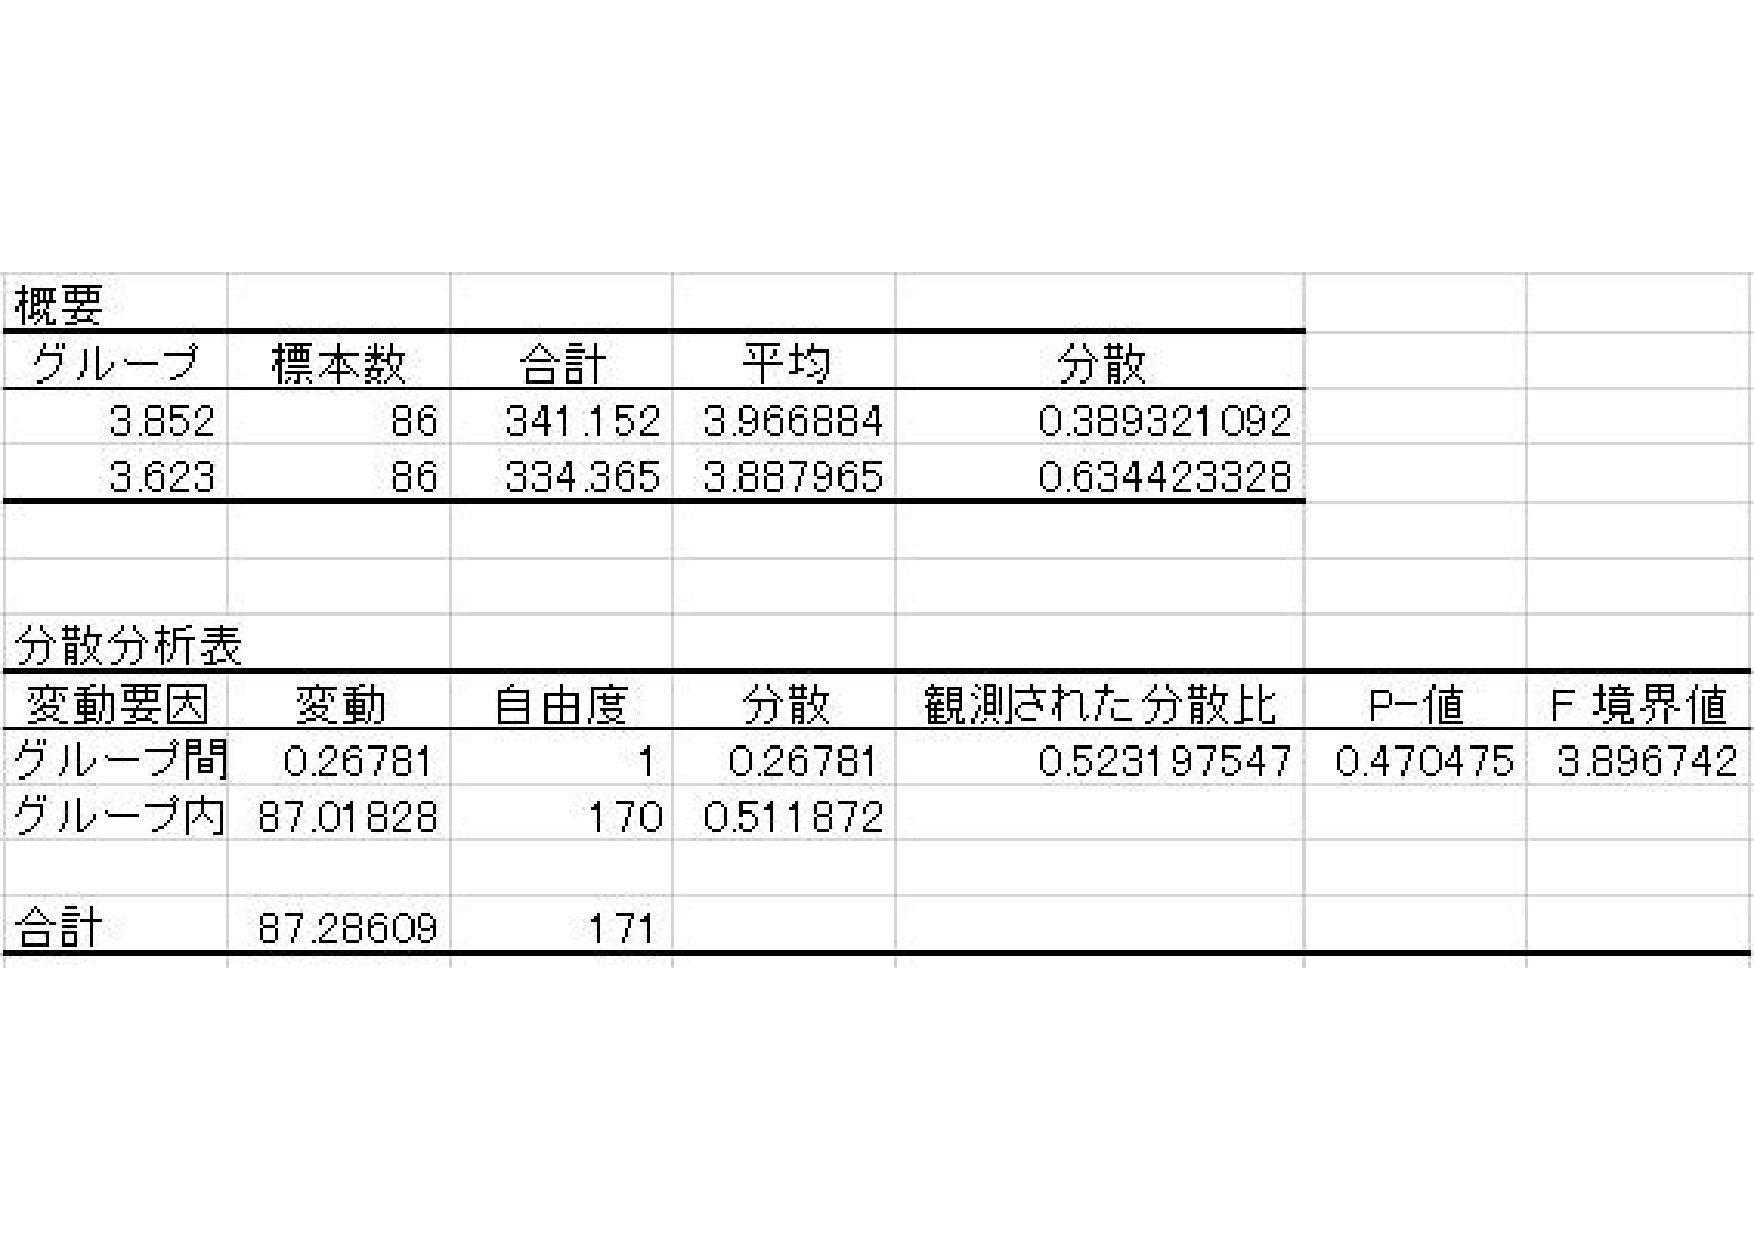
\includegraphics[width=12cm,clip]{reviewtoukei.pdf}
\caption{分散分析結果}
\label{reviewtoukei}

\end{figure}

\begin{figure}[htbp]

\centering
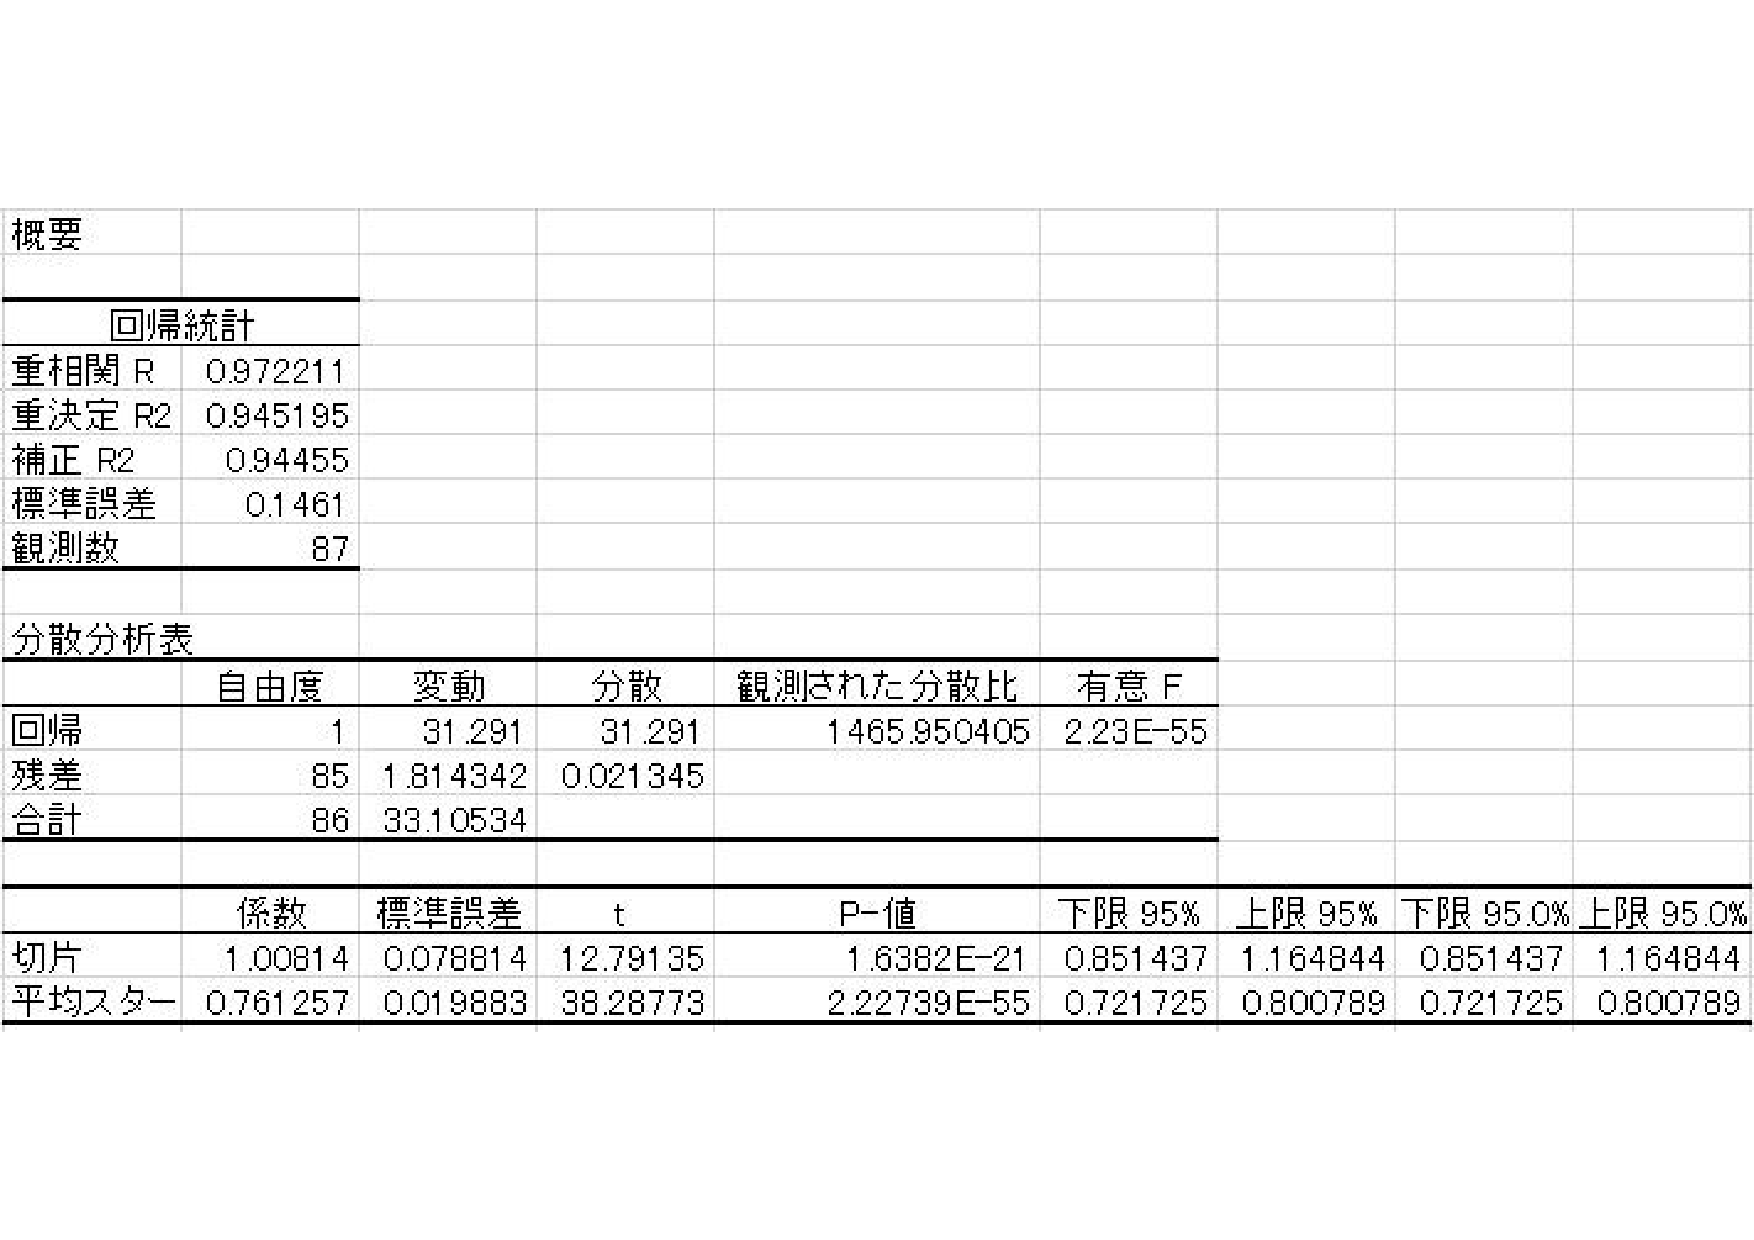
\includegraphics[width=12cm,clip]{reviewtoukei2.pdf}
\caption{回帰分析結果}
\label{reviewtoukei2}

\end{figure}


\clearpage

\begin{figure}[htbp]

\centering
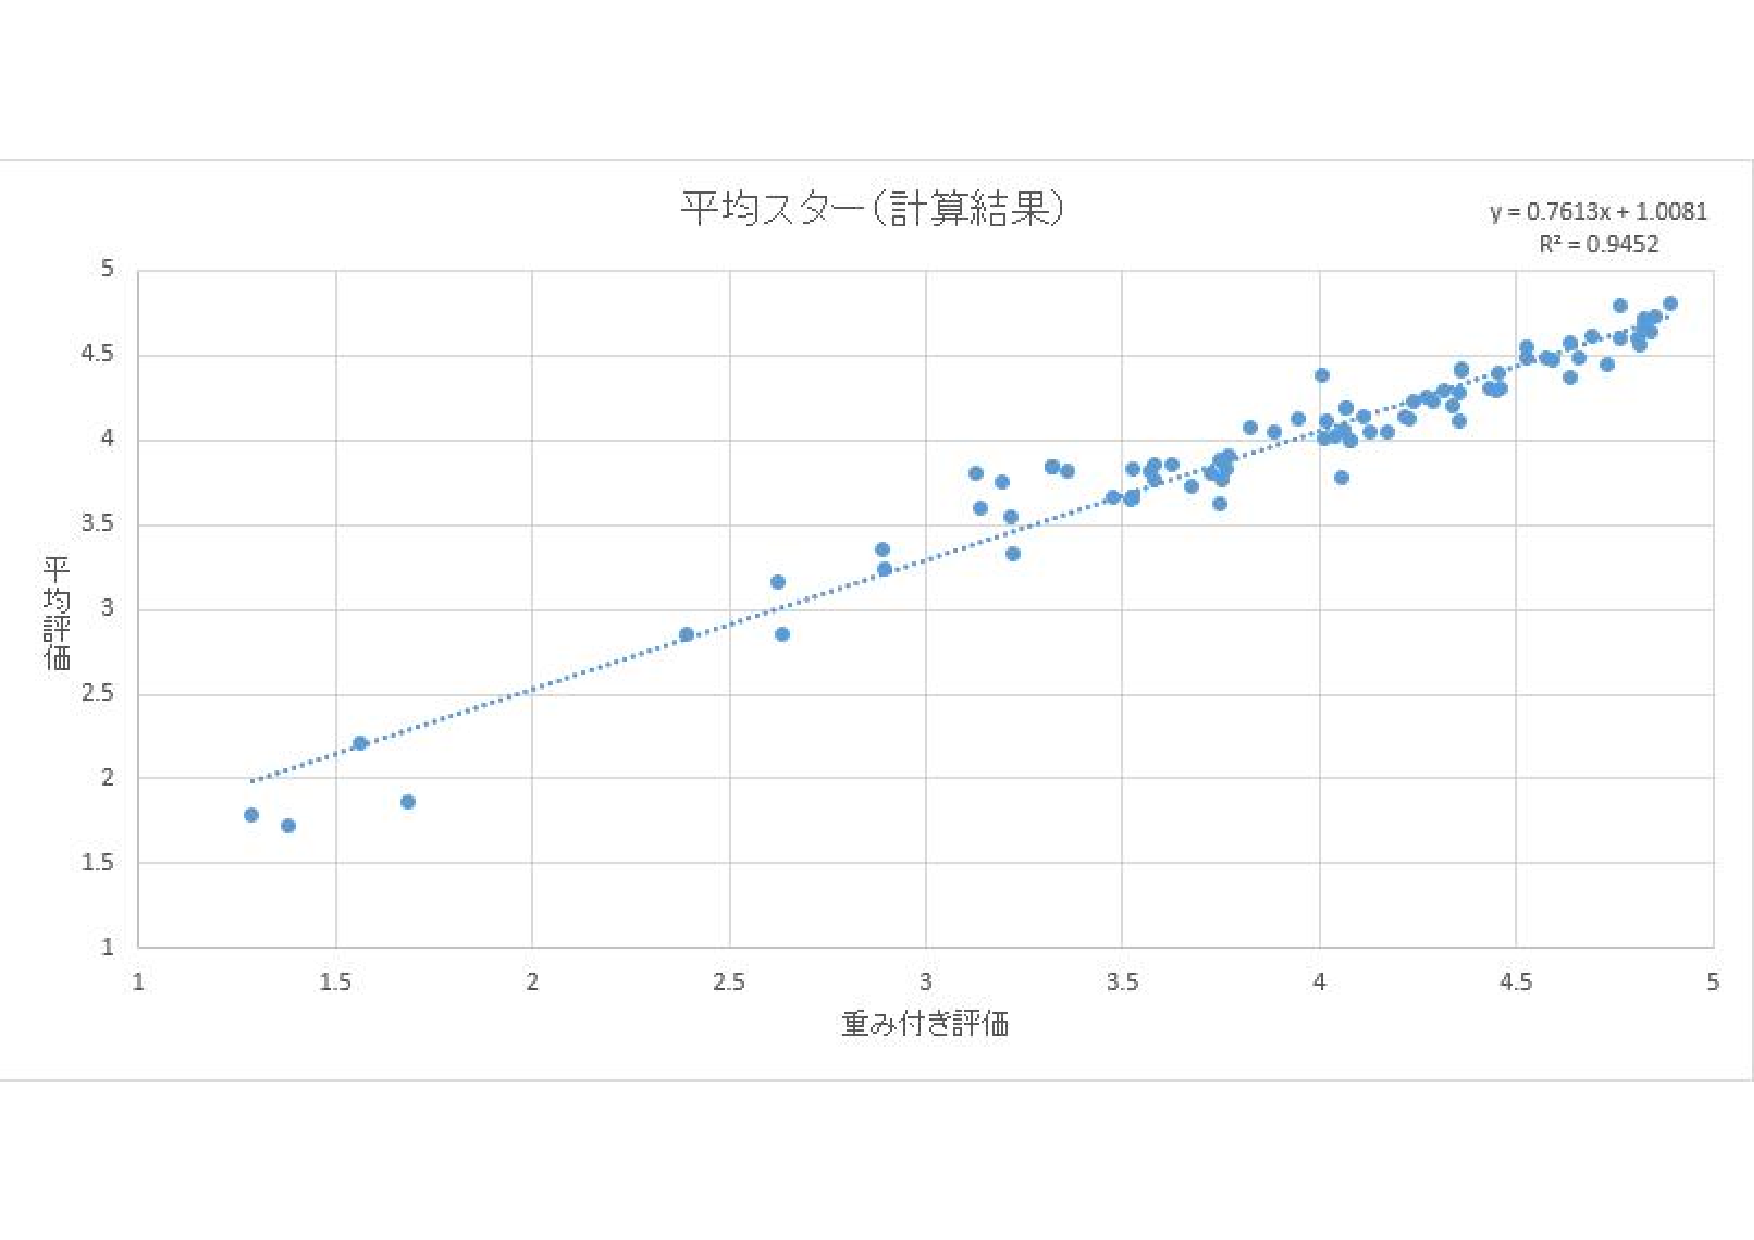
\includegraphics[width=12cm,clip]{sanpuzu.pdf}
\caption{重み付き評価と平均評価を比較した散布図}
\label{sanpuzu}

\end{figure}





89件のデータを調査した結果,各平均評価の平均値が3.966884,各重み付き評価の平均値が0.634423328,分散比が0.52319547,P-値が0.47045,F境界値が3.896742であった.
また,平均評価と重み付き評価の間で相関があり,相関係数は0.97という数値が算出された.
89件合計のレビュー数は27312件であった.
P-値が5%以下で,観測された分散比<F境界値であるため帰無仮説を棄却できる.
このことから,平均値と重み付き平均値の分散に差がないという帰無仮説を棄却でき,分散があることが分かる.

\clearpage

\section{「Amazonでの購入者」の項目を追加したデータの収集}


Amazon内で購入した,していない人物を分類分けしたものを加えて計9件のレビューデータを収集した.


\begin{table}[htb]
\label{reviewtoukei}
  \begin{center}
    \caption{レビューデータ統計}


\begin{tabular}{|r|r|r|r|}

\hline
件数 & 平均評価 & 重み付き評価 & 購入者のみの重み付き評価 \\
\hline\hline

1 &3.82747603833866 & 2.91061758213802 & 2.87358184764992\\


2 &4.70394736842105 & 3.58506864549148 & 3.12009303083278\\

3 &4.03418803418803 & 3.16443655814178 & 3.23882167280379\\

4 &3.94086021505376 & 2.68067931989644 & 2.62011975830101\\

5 &3.95394736842105 & 3.34345274330444 & 3.79410096426546\\

6 &3.171875 & 2.74595358109188 & 3.4445162332418\\

7 &4.34 & 3.25913258478392 & 3.41002949852507\\

8 &4.38144329896907 & 2.82412969201955 & 3.1474072084328\\

9 &2.18348623853211 & 2.81215114012391 & 2.28098117525035\\

	\hline
    \end{tabular}
  \end{center}
\end{table}


\begin{figure}[htbp]

\centering
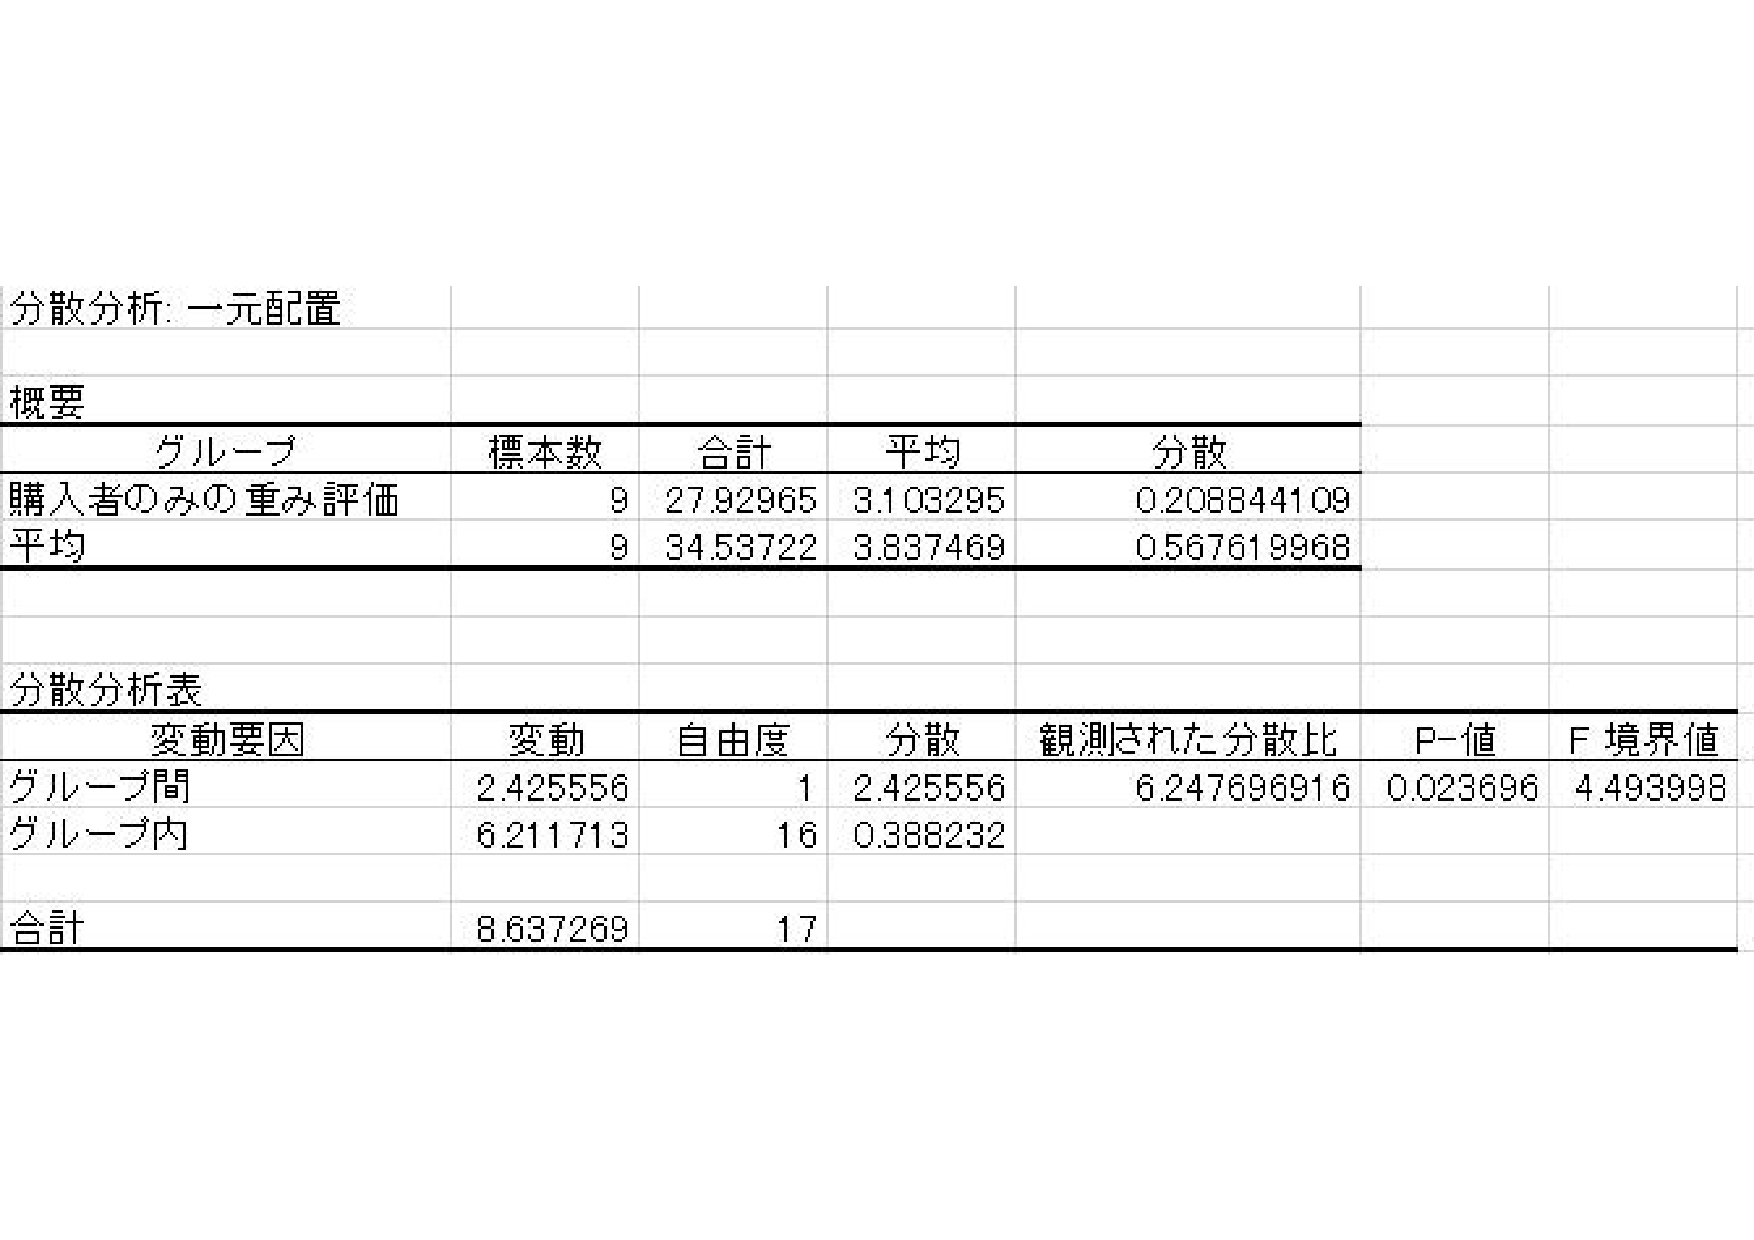
\includegraphics[width=12cm,clip]{reviewtoukei4.pdf}
\caption{購入者のみの項目での分散分析結果}
\label{reviewtoukei4}

\end{figure}

\clearpage

\begin{figure}[htbp]

\centering
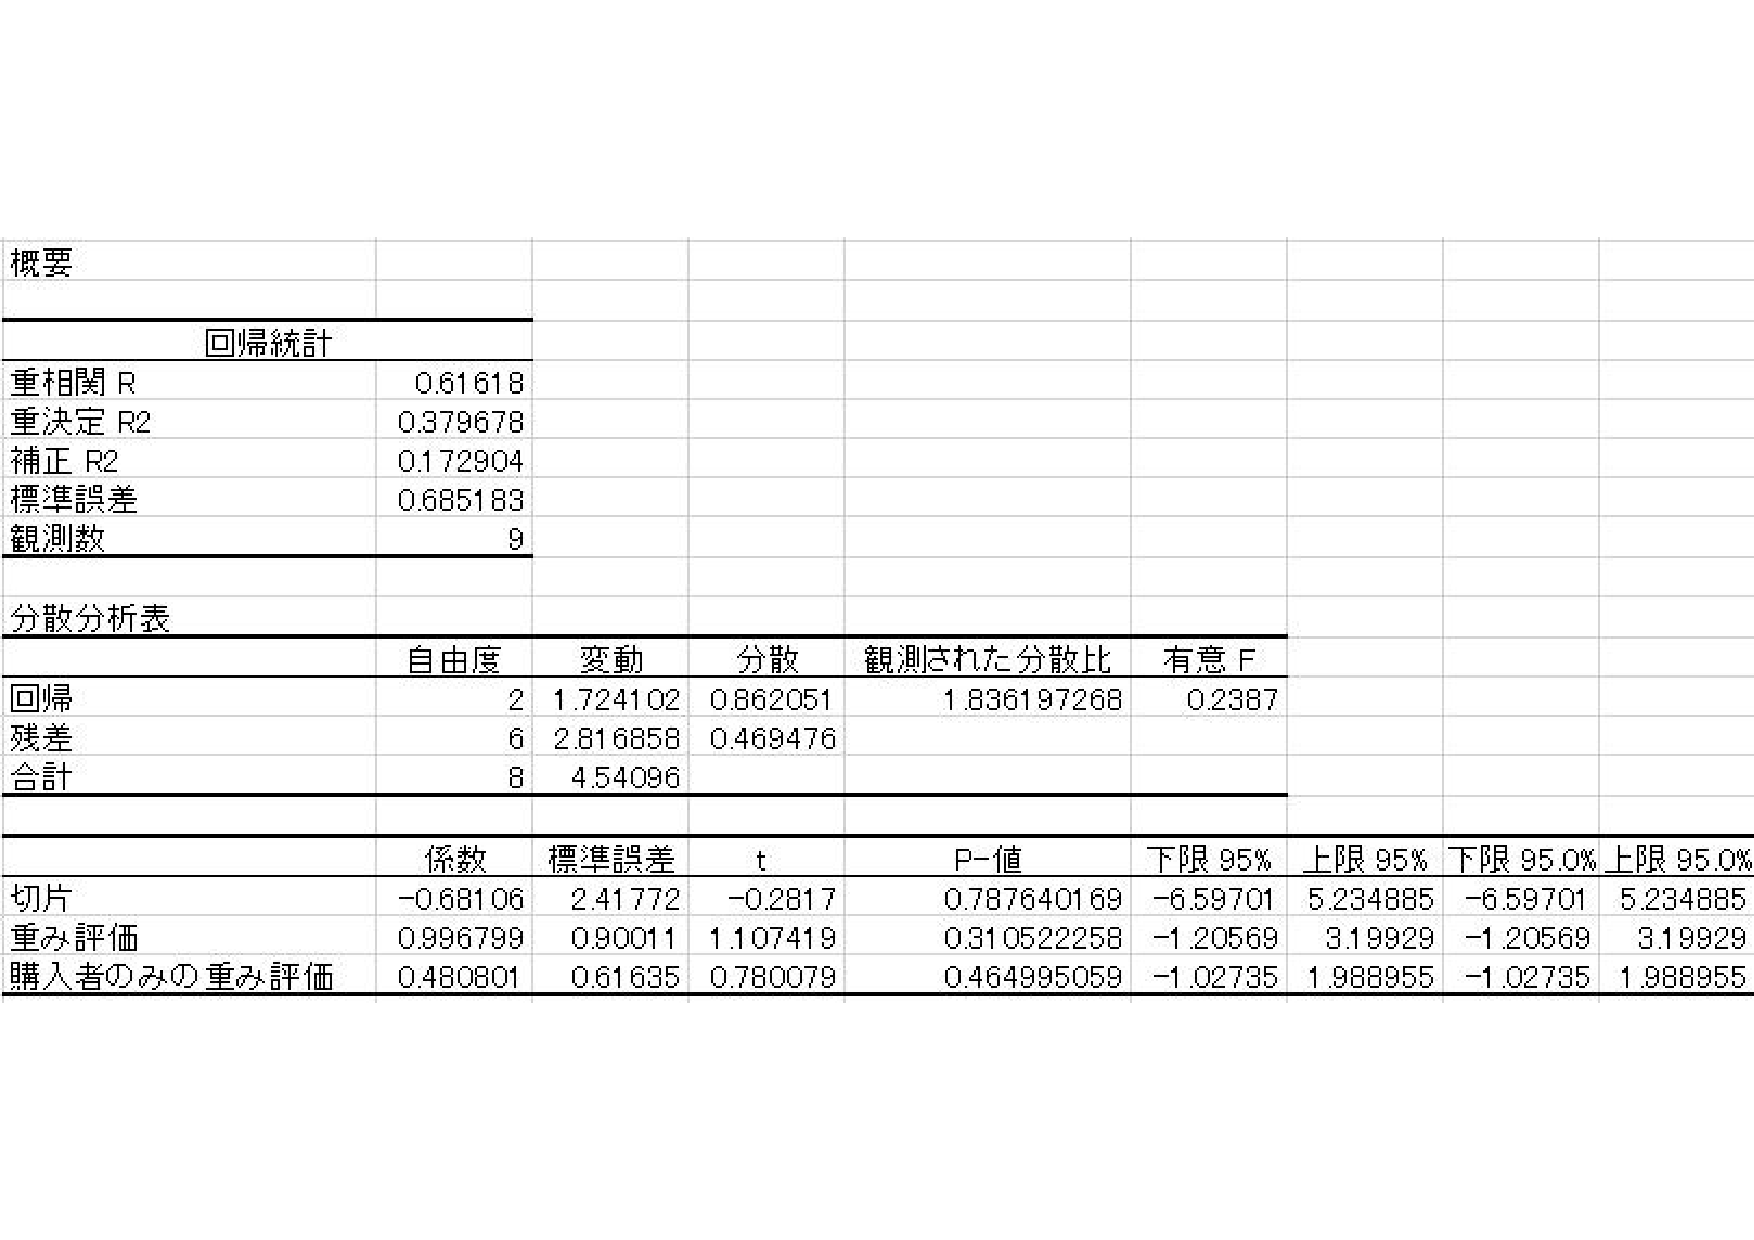
\includegraphics[width=12cm,clip]{reviewtoukei3.pdf}
\caption{購入者のみの項目での回帰分析結果}
\label{reviewtoukei3}

\end{figure}



\begin{figure}[htbp]

\centering
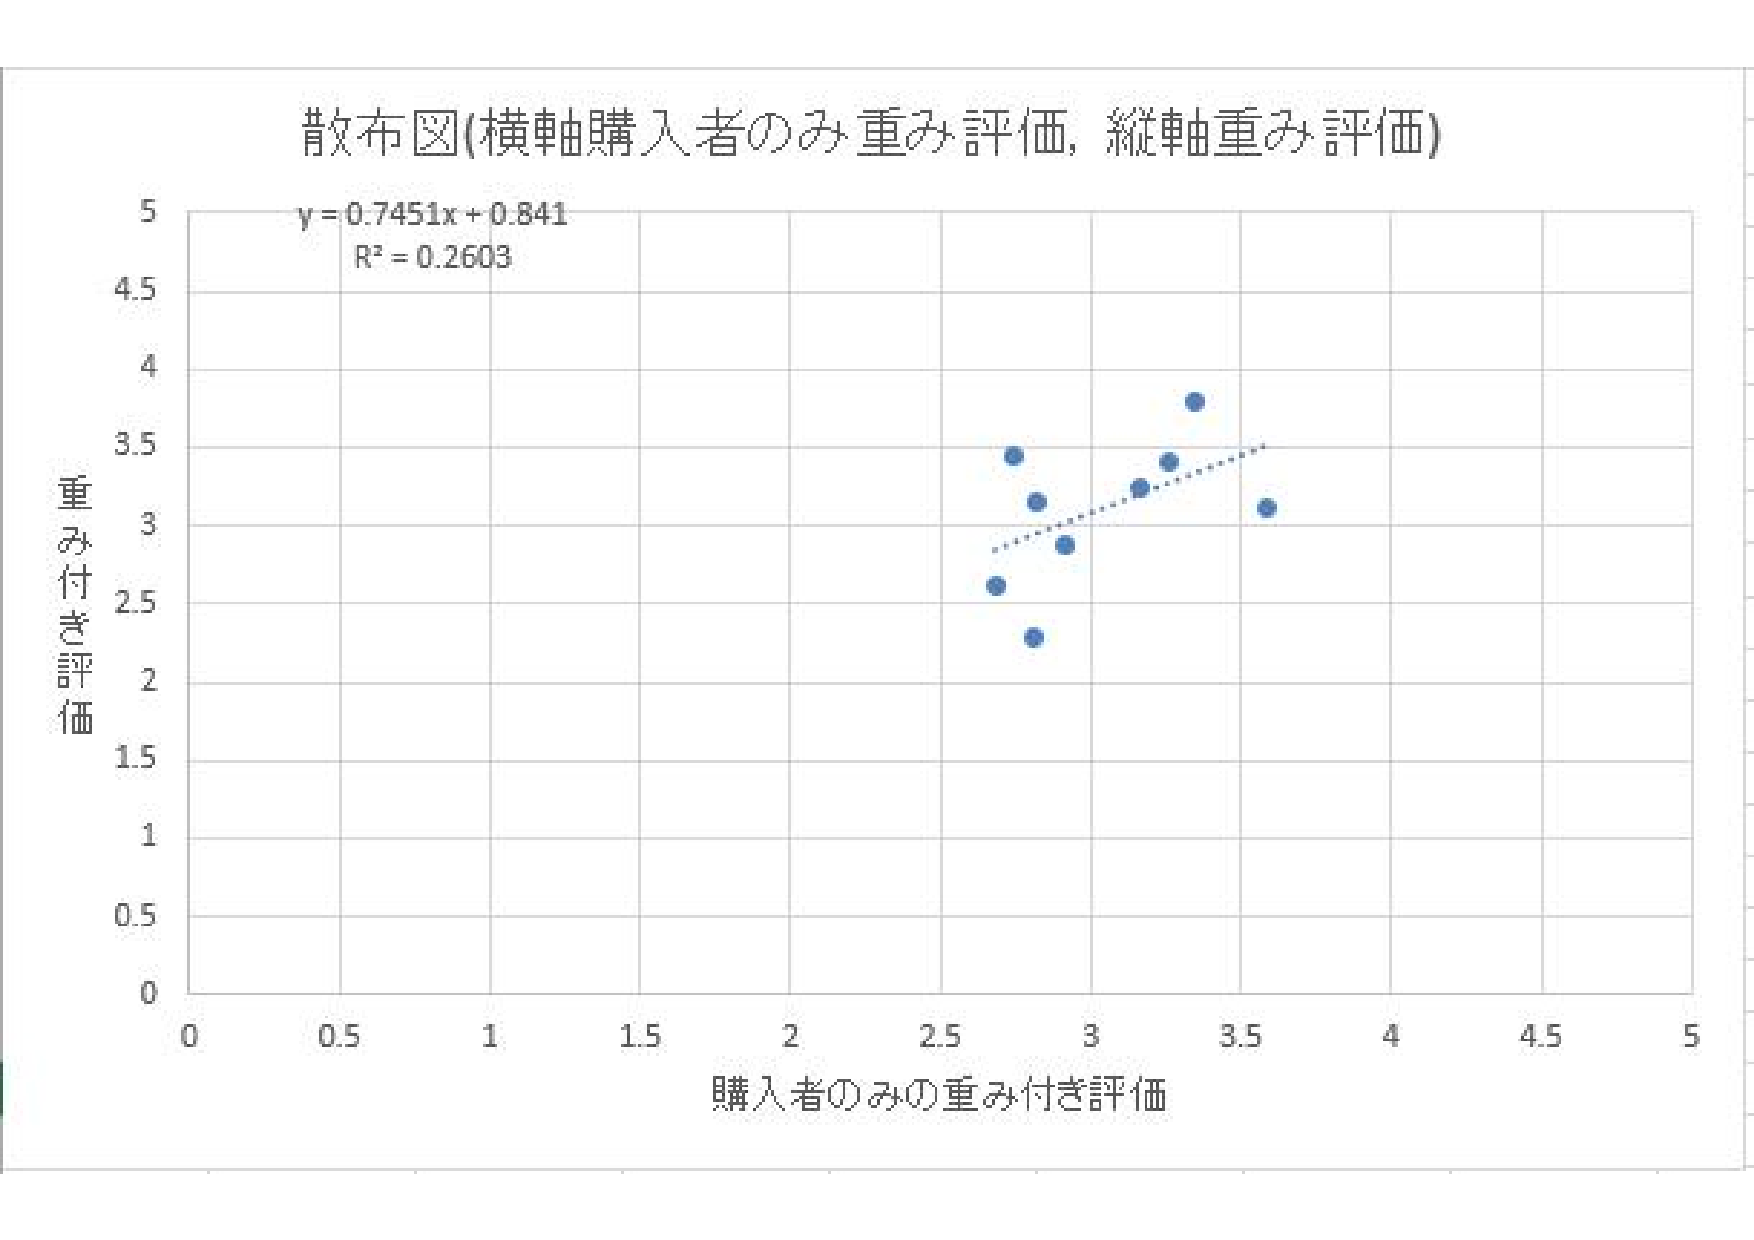
\includegraphics[width=12cm,clip]{sanpuzu2.pdf}
\caption{購入者のみの重み付き評価と重み付き評価を比較した散布図}
\label{sanpuzu2}

\end{figure}


\clearpage

\begin{figure}[htbp]

\centering
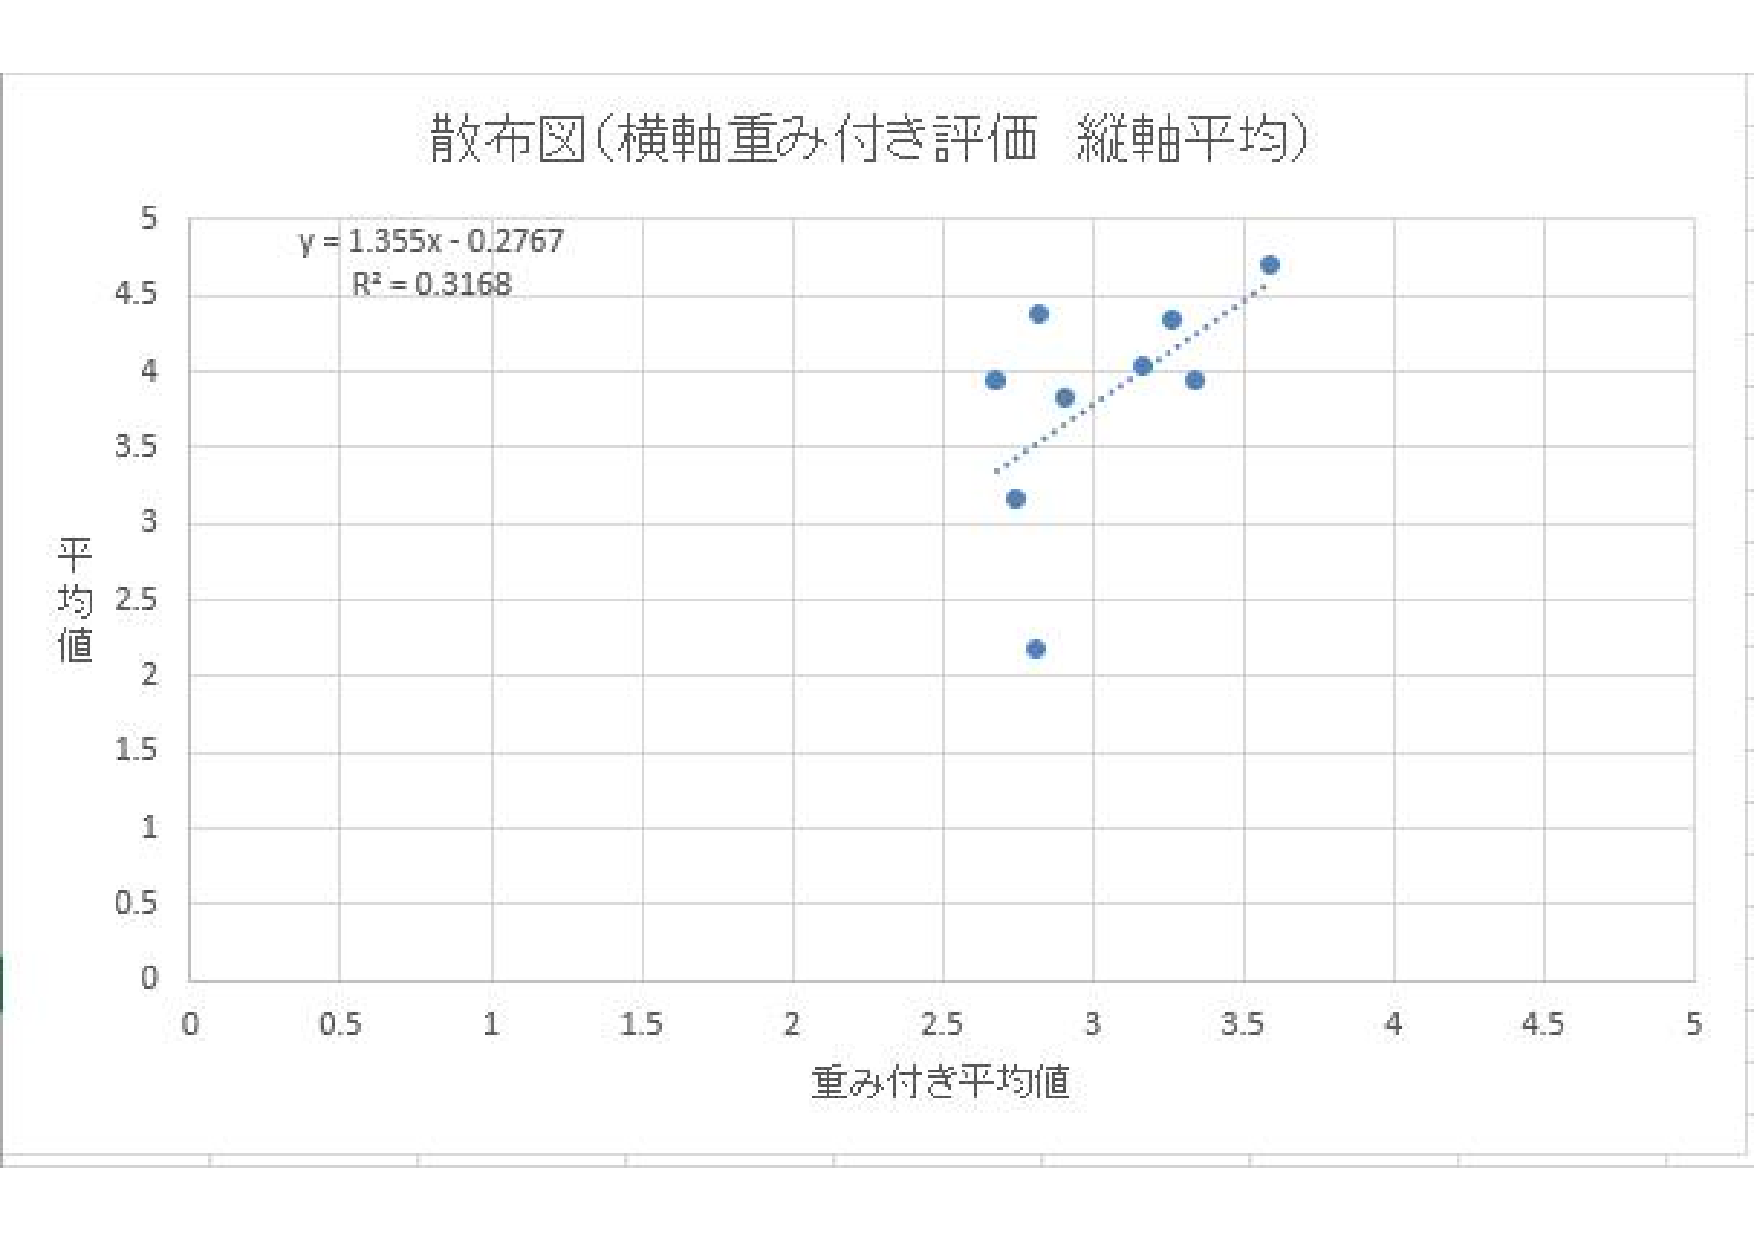
\includegraphics[width=12cm,clip]{sanpuzu3.pdf}
\caption{購入者のみの重み付き評価と平均評価を比較した散布図}
\label{sanpuzu3}

\end{figure}

\begin{figure}[htbp]

\centering
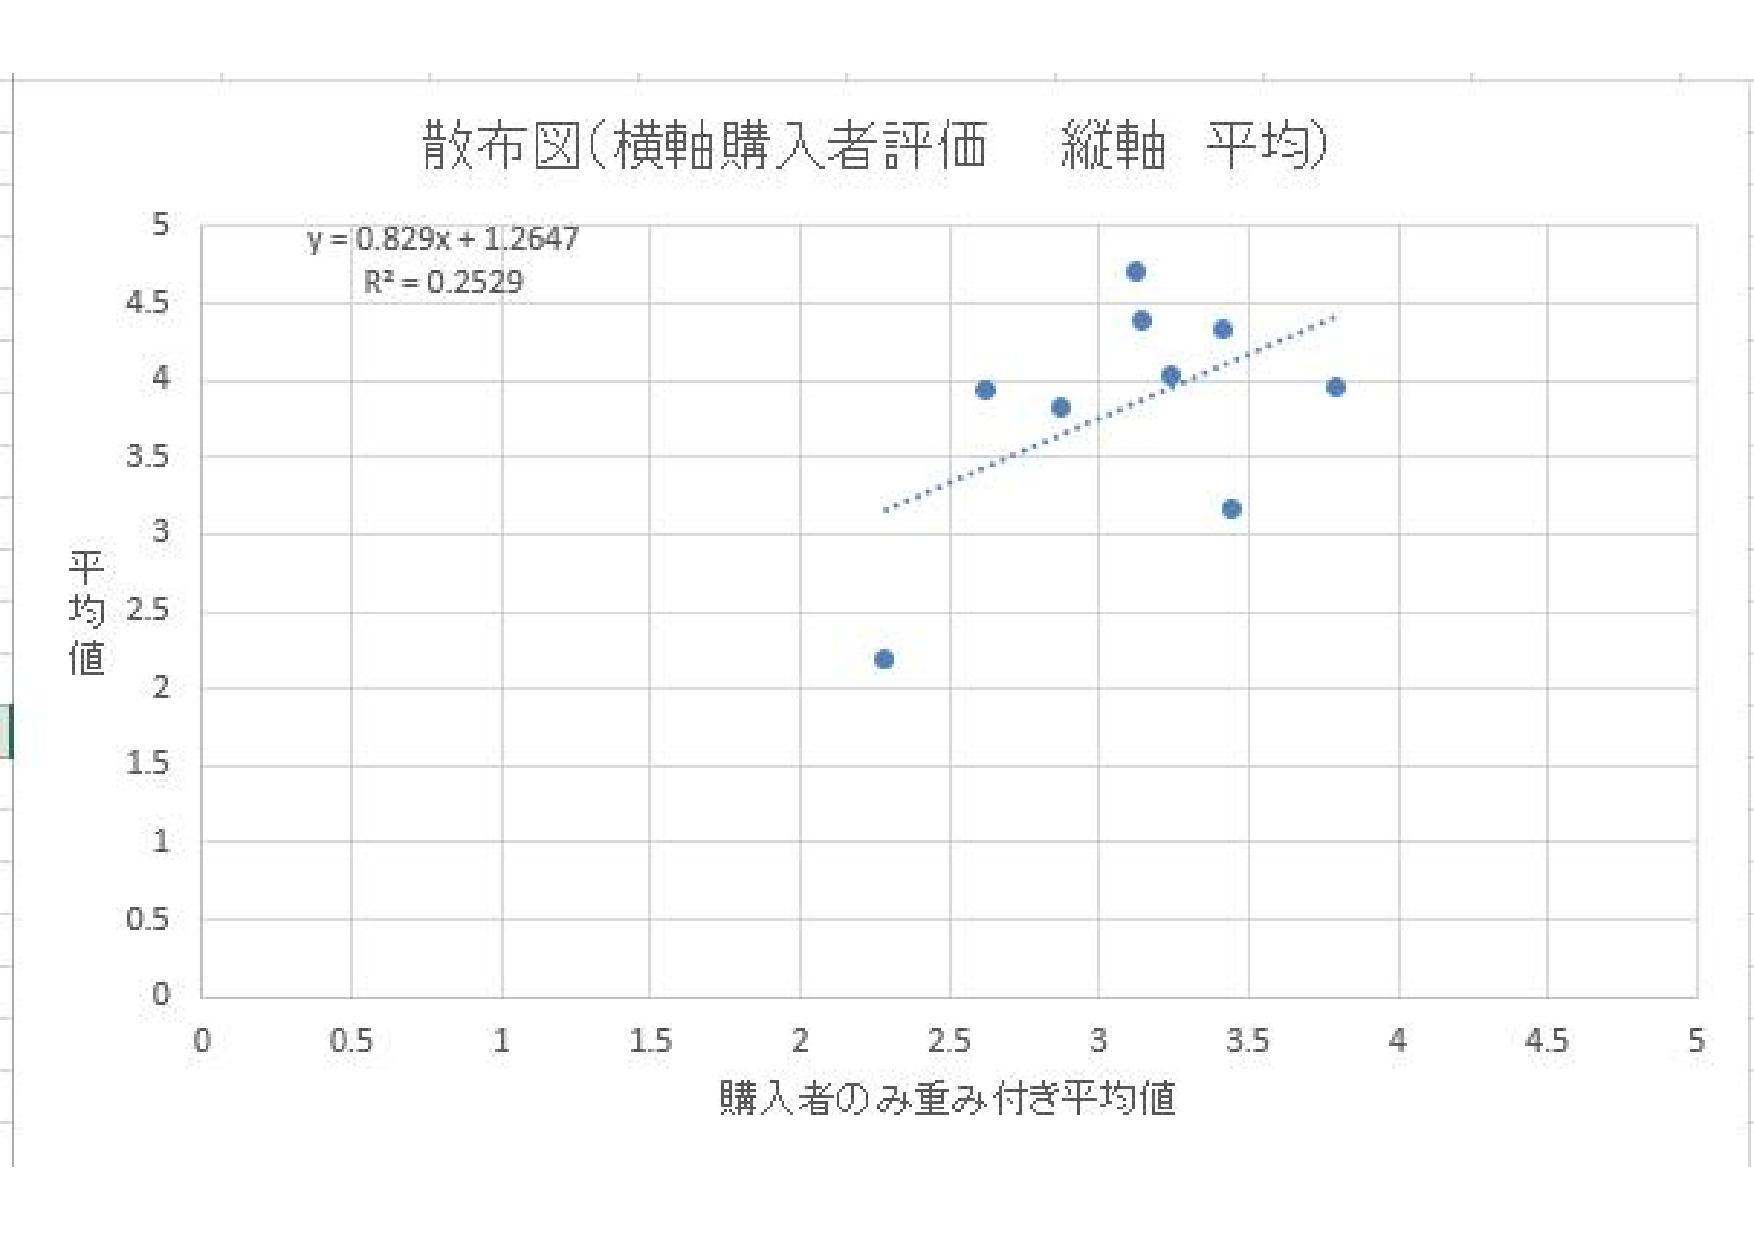
\includegraphics[width=12cm,clip]{sanpuzu4.pdf}
\caption{重み付き評価と平均評価を比較した散布図}
\label{sanpuzu4}

\end{figure}



\clearpage



9件のデータを調査した結果,各平均評価の平均値が3.103295,各重み付き評価の平均値が0.837469,分散比が6.247696916,P-値が0.029696,F境界値が4.44939998であった.
9件合計のレビュー数は1506件であった.
また,平均評価と購入した人物のみのレビューを使用した重み付き評価の散布図を作成し,相関係数は0.5という数値が算出された.

P-値が5%以下であるが,観測された分散比>F境界値であるため帰無仮説を棄却できない.
このことから,平均値と購入者のみの重み付き平均値の分散に差がないという帰無仮説を棄却できない.




\chapter{考察}

実際に見たレビューデータとして平均評価1である商品に皮肉で評価5をいれ,別の目的ならば有用,たて読みなどを記載したレビューの参考比率が高いものもあるが上記の収集方法ではそれらを選定するすべがない.

しかし,レビューデータの収集,手作業でのレビューデータ収集を行ったのでこれらに関係のある研究をする場合は収集方法,分析などで参考になる部分もあるだろう.

\subsubsection{研究における問題点}
JABA言語利用の下89件のレビューデータの収集を行った.

しかし,判断材料を増やす試みを行ったところ,JAVA言語の改変に手間取り想像以上の時間を要してしまった.

その結果エクセルを利用した手作業でのレビューデータ収集となったため,購入者のみの重み付き評価は9件という少ないレビューデータしか集まらなかった.
また,平均評価と重み付き平均のみの項目で調べた場合のレビュー数は27312件の量に対して,Amazonで購入した人のみに絞った項目を加えた場合のレビュー数は1506件と20倍近く少ない.

分析は行ったものの統計としては数が少なく判断材料として信頼できるものとはいえないものであろう.


\chapter{結論}


\section{相関係数による判断}


平均値と重み付き評価値は相関係数が0.97 であった.
購入者のみの重み付き評価値は相関係数0.5 であった.
よって購入者のみの相関係数のほうが相関が低いと言える.

このことから,レビューデータ全体から分析する方法に比べ,相関が低い結果が出た購入者に絞ったレビューデータから参考になったと答えた比率を分析すれば平均値より正確な商品の評価がわかる可能性が高いと言える.

目標である対象の商品が参考であるかの比率を踏まえた評価を出し,平均評価と比較することには成功した.購入者で絞った結果,そのほうが信頼できる評価になると推測できるが件数が少ないので断定できない.これらのツールを使いさらに項目数を増やすことで信頼できる度合いがさらに高くなることだろう.



\bibliographystyle{junsrt}
\bibliography{biblio}		%「biblio.bib」というファイルが必要.

\end{document}
